%\documentclass[conference]{IEEEtran}
%\documentclass[sigconf, anonymous]{acmart}
%\documentclass[11pt,letterpaper]{book}
\documentclass{llncs}
\pagestyle{plain}
%\usepackage[margin=1in]{geometry}
%\usepackage{times}
% \renewcommand*\sfdefault{cmss}
%\usepackage{amssymb,amsmath,amsfonts}
%\usepackage{chemarrow,extarrows}
\usepackage[linewidth=0.5pt]{mdframed}
%\usepackage{lipsum}
\usepackage{graphicx}
\usepackage{framed}
\usepackage{pythonhighlight}
%\usepackage{enumerate}
%\usepackage{enumitem}
%\usepackage{framed}
\usepackage{xcolor,xspace}
\usepackage{float,subfigure}
%\usepackage{etoolbox}
\usepackage{tabularx}
\usepackage{multicol}
\usepackage{multirow}

\usepackage{float}

%\fancyhf{} % Remove fancy page headers 
%\fancyhead[C]{Anonymous submission \#715 to ACM CCS 2017} % TODO: replace 9999 with your paper number
%\fancyfoot[C]{\thepage}

%\setcopyright{none} % No copyright notice required for submissions
%\acmConference[Anonymous Submission to ACM CCS 2017]{ACM Conference on Computer and Communications Security}{Due 19 May 2017}{Dallas, Texas}
%\acmYear{2017}

%\settopmatter{printacmref=false, printccs=true, printfolios=true} % We want page numbers on submissions


\usepackage{cite}
\usepackage{hyperref}

%\hyphenation{op-tical net-works semi-conduc-tor}
\hypersetup{colorlinks=true,citecolor=blue,filecolor=blue,linkcolor=blue,urlcolor=black}


\usepackage{colortbl}

\usepackage{paralist}
%\usepackage{pdfpages}
\usepackage{enumitem}
%\usepackage{float}
\usepackage{booktabs}
\usepackage[override]{cmtt}
%\usepackage[small]{titlesec}
\usepackage{color,xcolor}
%\usepackage{inconsolata,graphicx,color,eso-pic}
\usepackage{graphicx,color}
%\usepackage{amsmath,amssymb,stmaryrd}
%\usepackage{footnote}


\newcommand{\secparam}{\ensuremath{{\kappa}}}
\newcommand{\msf}[1]{\ensuremath{{\mathsf {#1}}}}
\newcommand{\mcal}[1]{\ensuremath{\mathcal {#1}}}
\newcommand{\fsgx}{{\color{darkred}{\ensuremath{\mcal{G}_{\textrm{sgx}}}}}\xspace}
\newcommand{\ftpm}{{\color{darkred}{\ensuremath{\mcal{G}_{\textrm{tpm}}}}}\xspace}
\newcommand{\fsgxrelax}{{\color{darkred}{\ensuremath{\widetilde{\mcal{G}}_{\textrm{sgx}}}}}\xspace}
\newcommand{\ftpmrelax}{{\color{darkred}{\ensuremath{\widetilde{\mcal{G}}_{\textrm{tpm}}}}}\xspace}
\newcommand{\foutsource}{{\color{darkred}{\ensuremath{\mcal{F}_{\textrm{outsrc}}}}}\xspace}
\newcommand{\fenclave}{{\color{darkred}{\ensuremath{\mcal{F}_{\textrm{enclave}}}}}\xspace}
\newcommand{\fsc}{{\color{darkred}{\ensuremath{\mcal{F}_{\textrm{sc}}}}}\xspace}
\newcommand{\fauth}{{\color{darkred}{\ensuremath{\mcal{F}_{\textrm{auth}}}}}\xspace}
\newcommand{\fstatefulobf}{{\color{darkred}{\ensuremath{\mcal{F}_{\textrm{statefulobf}}}}}\xspace}
\newcommand{\fsgxprime}{{\color{darkred}{\ensuremath{\widehat{\mcal{G}}_{\textrm{sgx}}}}}\xspace}
\newcommand{\fcom}{{\color{darkred}{\ensuremath{\mcal{F}_{\textrm{com}}}}}\xspace}
\newcommand{\ftwopc}{{\color{darkred}{\ensuremath{\mcal{F}_{\textrm{2pc}}}}}\xspace}
\newcommand{\fmpc}{{\color{darkred}{\ensuremath{\mcal{F}_{\textrm{mpc}}}}}\xspace}

\newcommand{\algM}{{\color{darkred}\ensuremath{\mcal{M}}}\xspace}
\newcommand{\algS}{{\color{black}\ensuremath{\mcal{S}}}\xspace}
\newcommand{\algC}{{\color{darkred}\ensuremath{\mcal{C}}}\xspace}
\newcommand{\algP}{{\ensuremath{\mcal{P}}}\xspace}
\newcommand{\algPi}{{\color{darkred}\ensuremath{\mcal{P}_i}}\xspace}
\newcommand{\algPj}{{\color{darkred}\ensuremath{\mcal{P}_j}}\xspace}
\newcommand{\algPone}{{\color{darkred}\ensuremath{\mcal{P}_1}}\xspace}
\newcommand{\algPn}{{\color{darkred}\ensuremath{\mcal{P}_n}}\xspace}
\newcommand{\algR}{{\color{darkred}\ensuremath{\mcal{R}}}\xspace}
\newcommand{\algA}{{\color{black}\ensuremath{\mcal{A}}}\xspace}
\newcommand{\algF}{{\color{black}\ensuremath{\mcal{F}}}\xspace}
\newcommand{\Fleader}{{\color{black}\ensuremath{\mcal{F}_{\rm leader}}}\xspace}
\newcommand{\Fsort}{{\color{black}\ensuremath{\mcal{F}_{\rm leader}}}\xspace}
\newcommand{\algB}{{\color{black}\ensuremath{\mcal{B}}}\xspace}
\newcommand{\adv}{{\color{darkred}\ensuremath{\mcal{A}}}\xspace}
\newcommand{\envi}{{\color{darkred}\ensuremath{{\mcal{Z}}}}\xspace}
\newcommand{\algZ}{{\ensuremath{{\mcal{Z}}}}\xspace}
\newcommand{\AZ}{{\ensuremath{({\mcal{A}}, \mcal{Z})}}\xspace}
\newcommand{\Sim}{\ensuremath{\msf{Sim}}\xspace}
%\newcommand{\st}{\ensuremath{{\it st}}\xspace}

\newcommand{\ct}{\ensuremath{{\sf ct}}\xspace}
\newcommand{\type}{\ensuremath{{\sf type}}\xspace}
\newcommand{\authenc}{\ensuremath{{\sf AE}}}
\renewcommand{\k}{\ensuremath{\secparam}}


\newcommand{\ie}{i.e.,\xspace}
\newcommand{\eg}{e.g.,\xspace}
\newcommand{\seq}{{\ensuremath{{\sf seq}}}\xspace}
\newcommand{\LOG}{{\ensuremath{{\sf LOG}}}\xspace}
\newcommand{\LOGell}{{\ensuremath{{\sf LOG}^{\langle \ell \rangle}}}\xspace}
\newcommand{\TXs}{{\ensuremath{{\sf TXs}}}\xspace}
\newcommand{\TX}{{\ensuremath{{\sf TX}}}\xspace}
\newcommand{\tx}{{\ensuremath{{\sf tx}}}\xspace}
%\newcommand{\m}{{\ensuremath{{\sf m}}}\xspace}
\newcommand{\lang}{{\ensuremath{{\cal L}}}\xspace}
\renewcommand{\L}{{\ensuremath{{\cal L}}}\xspace}
\newcommand{\keygen}{{\ensuremath{{\tt gen}}}\xspace}
\newcommand{\algVerify}{{\ensuremath{{\tt ver}}}\xspace}
\newcommand{\tspawn}{{\ensuremath{t_{\text{spawn}}}}\xspace}
\newcommand{\Tstart}{{\ensuremath{T_{\text{start}}}}\xspace}
\newcommand{\Tconfirm}{{\ensuremath{T_{\text{confirm}}}}\xspace}
\newcommand{\Tsnail}{{\ensuremath{T_{\text{snail}}}}\xspace}
\newcommand{\Tdummy}{{\ensuremath{T_{\bot}}}\xspace}
\newcommand{\Tend}{{\ensuremath{T_{\rm end}}}\xspace}
%\newcommand{\Tlarge}{{\ensuremath{T_{\rm end}}}\xspace}
\newcommand{\tildeb}{{\ensuremath{\widetilde{b}}}\xspace}
\newcommand{\hatb}{{\ensuremath{\widehat{b}}}\xspace}

\newcommand{\vrf}{{\ensuremath{{\sf VRF}}}\xspace}
\newcommand{\crs}{{\ensuremath{{\sf crs}}}\xspace}
\newcommand{\wtcrs}{{\ensuremath{\overline{\sf crs}}}\xspace}
\newcommand{\trap}{{\ensuremath{\tau}}\xspace}
\newcommand{\ek}{{\ensuremath{{\sf ek}}}\xspace}
\newcommand{\epk}{{\ensuremath{{\sf epk}}}\xspace}
\newcommand{\params}{{\ensuremath{{\sf params}}}\xspace}
\newcommand{\stmt}{{\ensuremath{{\sf stmt}}}\xspace}

\newcommand{\TODO}[1]{\noindent
\colorbox{green!20}{
\parbox{0.98\textwidth}{
#1
}}
}

\definecolor{goldenpoppy}{rgb}{0.99, 0.76, 0.0}
\definecolor{darkgreen}{rgb}{0,0.5,0}
\definecolor{lightblue}{RGB}{0,176,240}
\definecolor{darkblue}{RGB}{0,112,192}
\definecolor{lightpurple}{RGB}{124, 66, 168}
%\definecolor{orange}{rgb}{1,0.5,0}
\definecolor{grey}{RGB}{139, 137, 137}
\definecolor{maroon}{RGB}{178, 34, 34}
\definecolor{green}{RGB}{34, 139, 34}
\definecolor{types}{RGB}{72, 61, 139}
%\definecolor{gold}{rgb}{0.85, 0.65, 0.13}
\definecolor{gold}{rgb}{0.8, 0.33, 0.0}

\newcommand{\sred}[1]{{\color{maroon} \msf{#1}}}
\newcommand{\sblue}[1]{{\color{lightblue} {#1}}}
\newcommand{\spurple}[1]{{\color{lightpurple} \msf{#1}}}
\newcommand{\sorange}[1]{{\color{orange} \msf{#1}}}
\newcommand{\sgold}[1]{{\color{gold} {#1}}}
\newcommand{\smaroon}[1]{{\color{maroon} {#1}}}
\newcommand{\sgrey}[1]{{\color{grey} \msf{#1}}}
\newcommand{\sseablue}[1]{{\color{darkblue} {\bf #1}}}
\newcommand{\sdarkgreen}[1]{{\color{darkgreen} {#1}}}
\newcommand{\sdarkblue}[1]{{\color{darkblue} {#1}}}

\definecolor{darkgray}{gray}{0.3}
\newcommand{\cgray}[1]{{\color{darkgray} {#1}}}
\newcommand{\sgray}[1]{{\color{gray!100} {#1}}}
\newcommand{\skiptext}[1]{}
%\newcommand{\envi}{\ensuremath{{\sf env}}\xspace}
\newcommand{\msg}{\ensuremath{{{\sf m}}}\xspace}
\newcommand{\owf}{\ensuremath{{{\sf owf}}}\xspace}
\newcommand{\comm}{\ensuremath{{{\sf com}}}\xspace}
%\newcommand{\committee}{\ensuremath{{{\sf committee}}}\xspace}
\newcommand{\mpc}{\ensuremath{{{\sf mpc}}}\xspace}
\newcommand{\getr}{\ensuremath{{\leftarrow_{\$}}}\xspace}
\newcommand{\some}{{some \xspace}}

\newcommand{\Prot}{\ensuremath{{{\bf Prot}}}\xspace}

\newcommand{\install}{{\color{darkblue} \ensuremath{{{\tt install}}}\xspace}}
\newcommand{\resume}{{\color{darkblue} \ensuremath{{{\tt resume}}}\xspace}}
\newcommand{\getpk}{{\color{darkblue} \ensuremath{{{\tt getpk}}}\xspace}}
\newcommand{\corrupt}{{\color{darkblue} \ensuremath{{{\tt corrupt}}}\xspace}}
\newcommand{\sign}{{\color{darkblue} \ensuremath{{{\tt sign}}}\xspace}}

\newcommand{\pkM}{\ensuremath{{\sf mpk}}\xspace}
\newcommand{\skM}{\ensuremath{{\sf msk}}\xspace}



%%%
%%% FAN's MACRO 
%%% XXX
%%%
\newcommand{\onrcv}{\xspace\sblue{On~receive}\xspace}
\newcommand{\oninp}{\xspace\sblue{On~input}\xspace}
\newcommand{\oncall}{\xspace\sblue{On~call}\xspace}

\newcommand{\onrcvonce}{\xspace\sdarkgreen{On~receive}\xspace}
\newcommand{\oninponce}{\xspace\sdarkgreen{On~input}\xspace}
\newcommand{\pcforall}{{\bf for all}\xspace}
%\renewcommand{\pcreturn}{output\xspace}
%\renewcommand{\pcif}{if\xspace}
%\renewcommand{\pcelse}{else\xspace}
%\renewcommand{\pcfor}{for\xspace}
%\renewcommand{\pcthen}{then\xspace}

\newcommand{\progcomment}[1]{\cgray{\small \it //~#1}}

% vars
\newcommand{\inpfsgx}{{\ensuremath{{{\color{black}\sf inp}}}}}
\newcommand{\inp}{{\ensuremath{{{\color{black}\sf inp}}}}}
\newcommand{\outpfsgx}{{\ensuremath{{{\color{black}\sf outp}}}}}
\newcommand{\outp}{{\ensuremath{{{\color{black}\sf outp}}}}}
\newcommand{\regfsgx}{{\ensuremath{{{\color{black}\sf reg}}}}}

% keywords
\newcommand{\memfsgx}{{\ensuremath{\sf{{\color{black}mem}}}}}
\newcommand{\prog}{{\ensuremath{\sf{{\color{black}prog}}}}}
\newcommand{\progfsgx}{{\ensuremath{\sf{{\color{black}prog}}}}}
\newcommand{\iffsgx}{{\xspace{{\color{black}if}}\xspace}}

% operations
\newcommand{\assertfsgx}{{assert}\xspace}
\newcommand{\recordfsgx}{{record}\xspace}
\newcommand{\sendfsgx}{{\color{darkblue}{asend}}\xspace}
\newcommand{\secsendfsgx}{{\color{darkblue}{ssend}}\xspace}
\newcommand{\letfsgx}{{let}\xspace}
\newcommand{\returnfsgx}{{return}\xspace}

% strings
\newcommand{\stringfsgx}[1]{{\color{brown}\textrm{``{#1}''}}}
\newcommand{\party}[1]{{{\color{darkred}#1}}\xspace}
\newcommand{\func}[1]{\ensuremath{{\color{darkred}\mcal{#1}}}\xspace}

% lineno
\newcommand{\lnn}[1]{\small{\texttt{#1}}\xspace}


\usepackage{boxedminipage}
\usepackage{url}
\usepackage{graphicx}
%\usepackage{subcaption}
\usepackage{color}
\usepackage{xspace}
%\usepackage{multirow}
\let\proof\relax 
\let\endproof\relax
\usepackage{amsmath,amsthm,amstext,amssymb,amsfonts,latexsym}

%\usepackage{wrapfig}
\usepackage{algorithm}
\usepackage[noend]{algpseudocode}
\usepackage{algorithmicx}


\definecolor{darkred}{rgb}{0.5, 0, 0}
\definecolor{darkgreen}{rgb}{0, 0.5, 0}
\definecolor{darkblue}{rgb}{0,0,0.5}


%\lhead{\thepage \quad \quad \quad Ensighta Security Inc.}
%\rhead{Topic \# A10-013 \quad Proposal \# Army SBIR 2010.1}
%\lhead{\thepage}
%\chead{}
%\fancyfoot{}
%\chead{Ensighta Security Inc.}
%\setpagewiselinenumbers
%\linenumbers
%\pagewiselinenumbers

%\setlength{\textwidth}{7in} \setlength{\textheight}{9.62in}

%\usepackage{breakurl}
%\def\baselinestretch{0.97}
% center the one-line caption of a figure.
%\centerfigcaptionstrue
%\newcommand\markx[2]{\mbox{}\marginpar{\raggedright\hspace{0pt}#1:#2}}
\newcommand\markx[2]{}
\newcommand\markme[1]{\markx{ME}{#1}}
\newcommand\markjim[1]{\markx{JIM}{#1}}
\newcommand\marka[1]{\markx{R1}{#1}}
\newcommand\markb[1]{\markx{R2}{#1}}
\newcommand\markc[1]{\markx{R3}{#1}}

\newcommand{\marknew}{}
\newcommand{\DB}{\mathbf{DB}}
\newcommand{\model}{\mathbf{\Omega}}

%\newcommand{\authnote}[2]{{\bf #1 : #2}}
%\newcommand{\authnote}[2]{}

\newcommand{\david}[1]{{\authnote{david}{#1}}}
%\newcommand{\runting}[1]{{\authnote{runting}{#1}}}
\newcommand{\runting}[1]{{\footnotesize\color{red}[runting: #1]}}
\newcommand{\futureresearch}[1]{{\footnotesize\color{red}[dawn: #1]}}
\newcommand{\jim}[1]{{\authnote{jim}{#1}}}
%\newcommand{\dawn}[1]{{\authnote{dawn}{#1}}}
\newcommand{\zk}[1]{{\authnote{zk}{#1}}}
\newcommand{\cody}[1]{{\authnote{cody}{#1}}}
\newcommand{\heng}[1]{{\authnote{heng}{#1}}}

%\newcommand{\subgcons}{churn-oblivious consensus\xspace}
%\newcommand{\subgconsbig}{Churn-Oblivious Consensus\xspace}
%\newcommand{\Subgcons}{Churn-oblivious consensus\xspace}

\newcommand{\subgcons}{sleepy consensus\xspace}
\newcommand{\subgconsbig}{Sleepy Consensus\xspace}
\newcommand{\Subgcons}{Sleepy consensus\xspace}

%\newcommand{\name}{CO$_2$\xspace}
\newcommand{\name}{\textsf{Libra}\xspace}

%\newcommand{\aname}{an Elixir\xspace}
%\newcommand{\Aname}{An Elixir\xspace}


\newcommand{\pid}{{\color{darkgray}\mathit{pid}}}
\newcommand{\idx}{{\color{darkgray}\mathit{idx}}}
\newcommand{\eid}{{\color{darkgray}\mathit{eid}}}
\newcommand{\sid}{{\color{darkgray}\mathit{sid}}}
\newcommand{\ssid}{{\color{darkgray}\mathit{ssid}}}
\newcommand{\sk}{\mathsf{sk}}
\newcommand{\pk}{\mathsf{pk}}
\newcommand{\vk}{\mathsf{vk}}
%\newcommand{\idx}{\mathit{idx}}
%\newcommand{\poly}{\mathit{poly}}
\newcommand{\pc}{{\tt pc}}
\newcommand{\op}{\ensuremath{\mathsf{op}}\xspace}
\newcommand{\reg}{{\tt reg}}
\newcommand{\regs}{{\tt regs}}
\newcommand{\raddr}{{\tt raddr}}
\newcommand{\waddr}{{\tt waddr}}

\newcommand{\multicast}{{multicast}\xspace}
\newcommand{\multicasts}{{multicasts}\xspace}



\newcommand{\Path}{{\sf path}}
\newcommand{\dataopram}{\ensuremath{{\sf data}\text{-}{\sf OPRAM}}\xspace}
\newcommand{\posopram}{\ensuremath{{\sf pos}\text{-}{\sf OPRAM}}\xspace}
\newcommand{\posoprams}{\ensuremath{{\sf pos}\text{-}{\sf OPRAM}\text{s}}\xspace}
%\newcommand{\root}{{\sf root}}


\newcommand{\data}{{\ensuremath{\mathsf{data}}}\xspace}
\newcommand{\addr}{{\ensuremath{\mathsf{addr}}}\xspace}
\newcommand{\phaddr}{{\ensuremath{\mathsf{phaddr}}}\xspace}
\newcommand{\fetched}{{\ensuremath{\mathsf{fetched}}}\xspace}
\newcommand{\wdata}{{\tt wdata}}
\newcommand{\rdata}{{\tt rdata}}
\newcommand{\OPRAM}{{\sf OPRAM}}
\newcommand{\rlvl}{d}
\newcommand{\RLVL}{D}
\newcommand{\rpos}{{\sf rpos}}
\newcommand{\lpos}{{\sf lpos}}
\newcommand{\aux}{{\sf aux}}
\newcommand{\elem}{{\sf elem}}
\newcommand{\pair}{{\sf pair}}
\newcommand{\used}{{\beta}}
\newcommand{\arr}{{\sf arr}}
\newcommand{\negl}{{\sf negl}}
\newcommand{\reqs}{{\sf reqs}}
%\newcommand{\bLeft}{{\sf b}_0}
%\newcommand{\bRight}{{\sf b}_1}


\newcommand{\N}{\mathbb{N}}
%\newcommand{\G}{\mathbb{G}}
\newcommand{\Z}{\mathbb{Z}}
\newcommand{\F}{\mathbb{F}}

\newcommand{\SEE}{SEE\xspace}
\newcommand{\aSEE}{a SEE\xspace}
\newcommand{\ignore}[1]{}
\newcommand{\etal}{\textit{et al.}\xspace}

\renewcommand{\paragraph}[1]{\smallskip\noindent\textbf{#1}}
\newcommand{\squish}{
      \setlength{\topsep}{0pt}
      \setlength{\itemsep}{0ex}
      \vspace{-1ex}
      \setlength{\parskip}{0pt}}


\newcommand{\pksgx}{\ensuremath{{\sf pk}_{\textrm{sgx}}}}
\newcommand{\sksgx}{\ensuremath{{\sf sk}_{\textrm{sgx}}}}
\newcommand{\user}{\ensuremath{{\sf U}}}



\newcounter{task}
\newenvironment{task}[1]{ \refstepcounter{task} \paragraph{Task T\arabic{task}: #1}}{}


\newtheorem{protocol}{Protocol}
\newtheorem{construction}{Construction}
%\newtheorem{theorem}{Theorem}
%\newtheorem{remark}{Remark}
%\newtheorem{conjecture}{Conjecture}
%\newtheorem{corollary}{Corollary}
%\newtheorem{lemma}{Lemma}
%\newtheorem{proposition}{Proposition}
\newtheorem{fact}{Fact}
%\newtheorem{claim}{Claim}
\newtheorem{assumption}{Assumption}

%{
%\theoremstyle{definition}
%\newtheorem{definition}{Definition}
%}



\newcommand{\elainefix}[1]{{\footnotesize\color{magenta}[Elaine: #1]}}

\newcommand{\hubert}[1]{{\footnotesize\color{red}[Hubert: #1]}}
%\newcommand{\flo}[1]{\textcolor{blue}{[\textsf{Florian:  #1}]}}
%\newcommand{\dawn}[1]{\textcolor{blue}{[\textsf{Dawn:  #1}]}}
%\renewcommand{\elaine}[1]{}
%\renewcommand{\dawn}[1]{}
%\renewcommand{\fan}[1]{}
\newcommand{\babis}[1]{{\footnotesize\color{magenta}[Babis: #1]}}
%\newcommand{\weikai}[1]{{\footnotesize\textcolor{blue}{[\textsf{WK:  #1}]}}}
\newcommand{\tiancheng}[1]{{\footnotesize\textcolor{purple}{[\textsf{Tiancheng: #1}]}}}
\newcommand{\yupeng}[1]{{\color{red}[Yupeng: #1]}}

\newcommand{\dawn}[1]{{\color{blue}[Dawn: #1]}}


  %\renewcommand{\elaine}[1]{}
  \renewcommand{\tiancheng}[1]{}
  \renewcommand{\yupeng}[1]{}
  \renewcommand{\babis}[1]{}
  \renewcommand{\dawn}[1]{}

\newcommand{\es}{EbN\xspace}

\newcounter{cnt:challenge}

%\urlstyle{sf}

\newcommand{\elainetodo}[1]{%
\noindent    \colorbox{red!20}{%
\parbox{\textwidth}{
elaine: \\
 #1
    }
}
}

\newcommand{\rb}[1]{\colorbox{blue!20}{#1}}
\newcommand{\wt}[1]{{#1}}

%======================Yupeng =========

\newcommand{\tV}{\tilde{V}}
\newcommand{\tadd}{\tilde{add}}
\newcommand{\tmult}{\tilde{mult}}
\newcommand{\binary}{\{0,1\}}
\newcommand{\V}{\mathcal{V}}
\renewcommand{\P}{\mathcal{P}}
\renewcommand{\S}{\mathcal{S}}
\newcommand{\A}{\mathcal{A}}
\newcommand{\VPD}{\mathsf{VPD}}


\newcommand{\accept}{\mathsf{accept}}
\newcommand{\reject}{\mathsf{reject}}
\newcommand{\pp}{\mathsf{pp}}
\newcommand{\vp}{\mathsf{vp}}
\newcommand{\com}{\mathsf{comm}}
\newcommand{\KeyGen}{\mathsf{KeyGen}}
\newcommand{\Commit}{\mathsf{Commit}}
\newcommand{\CheckComm}{\mathsf{CheckComm}}
\newcommand{\Open}{\mathsf{Open}}
\newcommand{\Verify}{\mathsf{Verify}}


%===============rafael's macros ==============
\newcommand{\commentout}[1]{}
\newcommand{\LA}{\mathit{LA}}
%\renewcommand{\state}{chain}
%\newcommand{\N}{\mathcal{N}}
\newcommand{\m}{\textsf{m}}
\renewcommand{\b}{\textsf{b}}
%\newcommand{\C}{\textsf{chain}}
\newcommand{\genesis}{\bot}
%\newcommand{\EXEC}{\textsf{EXEC}^{(\Pi,\C)}(\algA,\algZ,\secparam)}
\newcommand{\exec}{\textsf{EXEC}}
\newcommand{\EXEC}{\textsf{EXEC}^{\Pi}(\algA,\algZ,\secparam)}
\newcommand{\EXECF}{\textsf{EXEC}^{(\Pi^{p,p_f,R},\C^{p,p_f,R})}(\algA,\algZ,\secparam)}
\newcommand{\EXECL}{\textsf{EXEC}^{(\Pi, \Le)}(\algA,\algZ,\secparam)}
\newcommand{\Proc}{\ensuremath{P}}
\newcommand{\bc}{\textsc{bc}}
\newcommand{\add}{\textsf{add}}
\newcommand{\view}{\textsf{view}}
\newcommand{\outZ}{\textsf{view}_{\algZ}}
\newcommand{\gro}{\textsf{growth}}
\newcommand{\groUp}{\textsf{upper-growth}}
\newcommand{\quality}{\textsf{quality}}
\newcommand{\self}{\textsf{self-consistent}}
\newcommand{\consistent}{\textsf{consistent}}
\newcommand{\common}{\textsf{common}}
\renewcommand{\neg}{\textsf{negl}}
\newcommand{\groB}{\textsf{min-chain-increase}}
\newcommand{\groC}{\textsf{max-chain-increase}}
%===============end of rafael's macros ==============



%===============defs==============
\newcommand{\bin}{\ensuremath{{\sf Bin}}\xspace}
\newcommand{\Bin}{\ensuremath{{\sf Bin}}\xspace}
\newcommand{\vote}{\ensuremath{{\sf vote}}\xspace}
\newcommand{\voteset}{\ensuremath{{\sf V}}\xspace}
%\newcommand{\V}{\ensuremath{{\sf V}}\xspace}
\newcommand{\chain}{\ensuremath{{\sf chain}}\xspace}
\newcommand{\ch}{\ensuremath{{\sf ch}}\xspace}
\newcommand{\fruitchain}{\ensuremath{{\sf FruitChain}}\xspace}
\newcommand{\bchain}{\ensuremath{\Pi_{\rm blockchain}}\xspace}
\newcommand{\protname}{\ensuremath{\Pi_{\rm thunder}}\xspace}
\newcommand{\protthunder}{\ensuremath{\Pi_{\rm thunder}}\xspace}
\newcommand{\protella}{\ensuremath{\Pi_{\rm ella}}\xspace}
\newcommand{\protellaadapt}{\ensuremath{\Pi^*_{\rm ella}}\xspace}
%\newcommand{\protthunderbyz}{\ensuremath{\Pi^{\diamond}_{\rm thunder}}\xspace}
\newcommand{\protthunderbyz}{\ensuremath{\Pi_{\rm thunder}}\xspace}
%\newcommand{\protellabyz}{\ensuremath{\Pi^{\diamond}_{\rm ella}}\xspace}
\newcommand{\protellabyz}{\ensuremath{\Pi_{\rm ella}}\xspace}
\newcommand{\protthunderadapt}{\ensuremath{\Pi^*_{\rm thunder}}\xspace}
\newcommand{\protthunderadaptbyz}{\ensuremath{\Pi^\bullet_{\rm thunder}}\xspace}
\newcommand{\protellaadaptbyz}{\ensuremath{\Pi^\bullet_{\rm ella}}\xspace}
\newcommand{\protthundercomm}{\ensuremath{\widetilde{\Pi}_{\rm thunder}}\xspace}
\newcommand{\protellacomm}{\ensuremath{\widetilde{\Pi}_{\rm ella}}\xspace}
\newcommand{\fchain}{\ensuremath{{\sf fchain}}\xspace}
\newcommand{\chstate}{\ensuremath{{\Gamma}}\xspace}
\newcommand{\chainh}{\ensuremath{{\sf chain}}\xspace}
\newcommand{\chainreal}{\ensuremath{{\it chain}}\xspace}
\newcommand{\chainsreal}{\ensuremath{{\it chains}}\xspace}
\newcommand{\pks}{\ensuremath{{\sf pks}}\xspace}
\newcommand{\mpk}{\ensuremath{{\sf upk}}\xspace}
\newcommand{\msk}{\ensuremath{{\sf usk}}\xspace}
\newcommand{\upk}{\ensuremath{{\sf upk}}\xspace}
\newcommand{\usk}{\ensuremath{{\sf usk}}\xspace}
\newcommand{\cmt}{\ensuremath{{\sf cmt}}\xspace}
\newcommand{\txs}{\ensuremath{{\sf txs}}\xspace}
\newcommand{\timestamp}{\ensuremath{{\sf time}}\xspace}
\newcommand{\nonce}{\ensuremath{{\sf nonce}}\xspace}
\newcommand{\electpks}{\ensuremath{{\sf elect\_pks}}\xspace}
\newcommand{\electh}{\ensuremath{{\sf elect\_h}}\xspace}
\newcommand{\wait}{\ensuremath{2\omega}\xspace}
\newcommand{\waithash}{\ensuremath{{\omega}}\xspace}

\newcommand{\round}{\ensuremath{{\sf rnddown}}\xspace}
\newcommand{\digest}{\ensuremath{{\sf d}}\xspace}
\newcommand{\extract}{\ensuremath{{\sf extract}}\xspace}
%\newcommand{\extractbyz}{\ensuremath{{\sf extract}^\diamond}\xspace}
\newcommand{\extractbyz}{\ensuremath{{\sf extract}}\xspace}
\newcommand{\extractadapt}{\ensuremath{{\sf extract}^*}\xspace}
\newcommand{\extractbyzadapt}{\ensuremath{{\sf extract}^\bullet}\xspace}
\newcommand{\extractadaptbyz}{\ensuremath{{\sf extract}^\bullet}\xspace}
\newcommand{\strip}{\ensuremath{{\sf strip}}\xspace}
\newcommand{\myjoin}{\ensuremath{||}\xspace}
\newcommand{\records}{\ensuremath{{\sf extract}}\xspace}
\newcommand{\rec}{\ensuremath{{\sf txs}}\xspace}
\newcommand{\recf}{\ensuremath{{\sf rec}^{\langle f \rangle}}\xspace}
\newcommand{\fruit}{\ensuremath{{\sf f}}\xspace}
\newcommand{\fruits}{\ensuremath{{\sf fruits}}\xspace}
\newcommand{\extractpks}{\ensuremath{{\sf extractpks}}\xspace}
\newcommand{\extractnonce}{\ensuremath{{\sf extractnonce}}\xspace}
\newcommand{\extractpids}{\ensuremath{{\sf extractpids}}\xspace}
%\newcommand{\hash}{\ensuremath{{\sf H}}\xspace}
\newcommand{\Tepoch}{\ensuremath{T_{\text{epoch}}}\xspace}
\newcommand{\ellepoch}{\ensuremath{\ell_{\text{epoch}}}\xspace}
\newcommand{\epoch}{\ensuremath{{\textsf{epoch}}}\xspace}
\newcommand{\coin}{\ensuremath{{{\tt coin}}}\xspace}
\newcommand{\Coin}{\ensuremath{{{\sf Coin}}}\xspace}
%\newcommand{\Gsign}{\ensuremath{\mathcal{G}_{\text{sign}}}\xspace}
\newcommand{\Fca}{\ensuremath{\mathcal{F}_{\text{CA}}}\xspace}
\newcommand{\Gsign}{\ensuremath{\Sigma}\xspace}
\newcommand{\Fsimple}{\ensuremath{\mathcal{F}_{\text{tree}}}\xspace}
\newcommand{\Ftree}{\ensuremath{\mathcal{F}_{\text{tree}}}\xspace}
\newcommand{\Fvotes}{\ensuremath{\mathcal{F}_{\text{votes}}}\xspace}
\newcommand{\Ftreeadaptive}{\ensuremath{\mathcal{F}^*_{\text{tree}}}\xspace}
\newcommand{\Ftreehyb}{\ensuremath{\widetilde{\mathcal{F}}_{\text{tree}}}\xspace}
\newcommand{\Ftreehybadaptive}{\ensuremath{{\mathcal{F}}^*_{\text{hyb}}}\xspace}



\newcommand{\Ftreehybi}{\ensuremath{{\mathcal{F}}^{\langle 2 \rangle}_{\text{hyb}}}\xspace}
\newcommand{\Ftreehybt}{\ensuremath{{\mathcal{F}}^{\langle 3 \rangle}_{\text{hyb}}}\xspace}
\newcommand{\Ftreehybf}{\ensuremath{{\mathcal{F}}^{\langle 4 \rangle}_{\text{hyb}}}\xspace}
\newcommand{\Ftreehybg}{\ensuremath{{\mathcal{F}}^{\langle 5 \rangle}_{\text{hyb}}}\xspace}
\newcommand{\prothybi}{\ensuremath{{\Pi}^{\langle 2 \rangle}_{\text{hyb}}}\xspace}
\newcommand{\prothybt}{\ensuremath{{\Pi}^{\langle 3 \rangle}_{\text{hyb}}}\xspace}
\newcommand{\prothybf}{\ensuremath{{\Pi}^{\langle 4 \rangle}_{\text{hyb}}}\xspace}
\newcommand{\prothybg}{\ensuremath{{\Pi}^{\langle 5 \rangle}_{\text{hyb}}}\xspace}

\newcommand{\Ftreehybz}{\ensuremath{{\mathcal{F}}^{\langle 1 \rangle}_{\text{hyb}}}\xspace}
\newcommand{\prothybz}{\ensuremath{{\Pi}^{\langle 1 \rangle}_{\text{hyb}}}\xspace}
\newcommand{\kcorrupt}{\ensuremath{{\vec{k}}_{\rm corrupt}}\xspace}


\newcommand{\Ftreeprime}{\ensuremath{{\mathcal{F}}_{\text{bias}}}\xspace}
\newcommand{\Ftreestablepast}{\ensuremath{{\mathcal{F}}_{\text{stablepast}}}\xspace}
\newcommand{\protbasic}{\ensuremath{\Pi_{\text{sleepy}}}\xspace}
\newcommand{\protchain}{\ensuremath{\Pi_{\text{chain}}}\xspace}
\newcommand{\protchainreal}{\ensuremath{\widetilde{\Pi}_{\text{chain}}}\xspace}
\newcommand{\protdisc}{\ensuremath{\Pi_{\text{discount}}}\xspace}
\newcommand{\protadaptive}{\ensuremath{\Pi^*_{\text{sleepy}}}\xspace}
\newcommand{\protsimple}{\ensuremath{\Pi_{\text{ideal}}}\xspace}
\newcommand{\prothyb}{\ensuremath{\Pi_{\text{hyb}}}\xspace}
\newcommand{\prothybadaptive}{\ensuremath{\Pi^*_{\text{hyb}}}\xspace}
\newcommand{\protsimpleprime}{\ensuremath{{\Pi}_{\text{bias}}}\xspace}
\newcommand{\protbias}{\ensuremath{{\Pi}_{\text{bias}}}\xspace}
\newcommand{\protsig}{\ensuremath{\Pi_{\text{hyb}}}\xspace}
\newcommand{\protrealver}{\ensuremath{\Pi_{\text{realver}}}\xspace}
%\newcommand{\protpos}{\ensuremath{\Pi_{\text{CO}_2}}\xspace}
\newcommand{\protpos}{\ensuremath{\Pi_{\text{sleepy}}}\xspace}
\newcommand{\protstablepast}{\ensuremath{\Pi_{\text{stablepast}}}\xspace}
\newcommand{\ver}{\ensuremath{\tt ver}\xspace}
\newcommand{\ppt}{\ensuremath{\text{p.p.t.}}\xspace}
\newcommand{\poly}{\ensuremath{{\sf poly}}\xspace}
\newcommand{\ind}{\ensuremath{\overset{c}{\equiv}}\xspace}

\newcommand{\pids}{{\color{black}\mathsf{pids}}}
\newcommand{\tree}{{\ensuremath{\mathsf{tree}}}\xspace}
\newcommand{\E}{{\ensuremath{\mathbf{E}}}\xspace}


\newcommand{\shortsleep}{{\color{black}\widetilde{\Delta}}}
\newcommand{\leadertab}{{\color{black}{\sf Coin}}}
\newcommand{\committee}{{\ensuremath{\sf committee}}\xspace}

\newcommand{\alert}{alert\xspace}
\newcommand{\pmin}{\ensuremath{p_{\rm m}}\xspace}


\newcommand{\X}{{\bf X}\xspace}
\newcommand{\Y}{{\bf Y}\xspace}
%\newcommand{\Z}{{\bf Z}\xspace}
\newcommand{\T}{{\bf T}\xspace}
%\newcommand{\A}{{\bf A}\xspace}
\newcommand{\lshort}{\ensuremath{L}\xspace}
\newcommand{\llong}{\ensuremath{L_0}\xspace}
\newcommand{\lead}{{\sf lead}\xspace}
\newcommand{\good}{{\sf good}\xspace}
\newcommand{\forks}{{\sf forks}\xspace}
\newcommand{\linearize}{{\sf linearize}\xspace}
\newcommand{\trim}{{\sf trim}\xspace}
\newcommand{\ncrupt}{\ensuremath{N_{\rm crupt}}\xspace}
\newcommand{\nalert}{\ensuremath{N_{\rm alert}}\xspace}
\newcommand{\achain}{\ensuremath{{\sf accept}}\xspace}
\newcommand{\insist}{\ensuremath{{\sf insist}}\xspace}
\newcommand{\prefix}{\ensuremath{{\sf prefix}}\xspace}
\newcommand{\cuta}{\ensuremath{{\kappa_0}}\xspace}
%\newcommand{\cuti}{\ensuremath{{\kappa_0}}\xspace}
%\newcommand{\bad}{{\sf bad}\xspace}

\newcommand{\gsign}{\ensuremath{\mcal{G}_{\rm sign}^\Sigma}\xspace}
\newcommand{\Tconf}{\ensuremath{T_{\rm end}}\xspace}
\newcommand{\cc}{\ensuremath{{\sf CC}}\xspace}
\newcommand{\CC}{\ensuremath{{\sf CC}}\xspace}
\newcommand{\nizk}{\ensuremath{{\sf nizk}}\xspace}
\newcommand{\partany}{\ensuremath{{\sf Partition}}\xspace}


\newcommand{\ceil}[1]{{\lceil #1 \rceil}}
\newcommand{\Ceil}[1]{{\left\lceil #1 \right\rceil}}
\newcommand{\floor}[1]{{\lfloor #1 \rfloor}}
\newcommand{\Floor}[1]{{\left\lfloor {#1} \right\rfloor}}
\newcommand{\half}{\frac{1}{2}}

% algorithm env
\renewcommand{\Comment}[1]{{\hfill \small \it \textcolor{darkgray}{\quad// #1}}}
\algnewcommand{\parState}[1]{\State \parbox[t]{\dimexpr \linewidth - 1cm}{\strut #1\strut}}



\begin{document}
%
% paper title
% Titles are generally capitalized except for words such as a, an, and, as,
% at, but, by, for, in, nor, of, on, or, the, to and up, which are usually
% not capitalized unless they are the first or last word of the title.
% Linebreaks \\ can be used within to get better formatting as desired.
% Do not put math or special symbols in the title.

\begin{titlepage}
\title{\name: Succinct Zero-Knowledge Proofs with Optimal Prover Computation}
\author{}
\institute{}
\end{titlepage}
\maketitle
\begin{abstract}
   We present a new construction of zero-knowledge argument. The prover time of our scheme is optimal: $O(C)$ for a circuit of size $C$, up to a constant multiplicative factor more than evaluating the circuit. When the circuit is log-space uniform with depth $d$, the proof size and verification time of our scheme is $d\log C$. 
   
   Underlying our new zero knowledge argument scheme is a new variant of the interactive proof protocol by Goldwasser et al. 2008 with linear prover time, and an efficient approach to turn the protocol to zero-knowledge using small masking polynomials.
   
   The implementation of our scheme, \name, shows that it only takes 200 seconds to generate a proof for constructing a Merkle tree with 511 SHA256 hashes, which is the best among all existing zero-knowledge proof systems. The proof size and the verification time of our scheme are also competitive. 
    
    
\end{abstract}
%!TEX root = fastZKP.tex
\section{Introduction}\label{sec:intro}


Zero-knowledge proofs (ZKP) are cryptographic protocols between two parties, a \emph{prover} and a \emph{verifier}, in which the prover can convince the verifier about the validity of a statement without leaking any extra information beyond the fact that the statement is true.  Since they were first introduced by Goldwasser et al.~\cite{goldwasser1989knowledge}, ZKP protocols have evolved from pure theoretical constructs to practical implementations, achieving proof sizes  of just hundreds of bytes and verification times of several milliseconds, regardless of the size of the statement being proved. Due to this successful transition to practice, ZKP protocols have found numerous applications not only in the traditional computation delegation setting but most importantly in providing privacy of transactions in deployed cryptocurrencies (e.g., Zcash~\cite{zerocash}) as well as in other blockchain research projects (e.g., Hawk~\cite{kosba2016hawk}). 




 




 




Despite such progress in practical implementations, ZKP protocols are still notoriously hard to scale for large statements, due to a particularly high overhead on generating the proof. For most systems, this is primarily because the prover has to  perform a large number of cryptographic operations, such as exponentiation in an elliptic curve group. And to make things worse the asymptotic complexity of computing the proof is typically more than linear, e.g., $O(C\log C)$ or even $O(C\log^2 C)$, where $C$ is the size of the statement.

Unfortunately, as of today we are yet to construct a ZKP system whose prover time is \emph{optimal}, i.e., linear in the size of the statement $C$ (this is irrespective of whether the ZKP system has per-statement trusted setup, one-time trusted setup or no trusted setup at all). The only notable exception is the recent work by B{\"u}nz et al.~\cite{bulletproofs} that however suffers from linear verification time---for a detailed comparison  see Table~\ref{table:comp}. Therefore designing ZKP systems that enjoy linear prover time as well as succinct\footnote{In ZKP literature, ``succinct" is poly-logarithmic in the size of the statement $C$.} proof size and verification time is an open problem, whose resolution can have significant practical implications. 



\paragraph{Our contributions.} In this paper we propose \name, the first ZKP protocol with \emph{linear prover time} and \emph{succinct proof size and verification time} in the size of the arithmetic circuit representing the statement $C$\footnote{The verification time is succinct in our protocol only when the circuit is log-space uniform. For all ZKP protocols without per-circuit setup, this is the best that can be achieved, as the verifier must read the entire circuit, which takes linear time in the worst case. We always refer to log-space uniform circuits when we say our scheme is succinct in this paper, to differentiate from schemes with linear verification time on all circuits (irrespective of whether the circuits are log-space uniform or not). Schemes such as \textsf{libSTARK}~\cite{libstark}, \textsf{zkVSQL}~\cite{zkvpd} and \textsf{Hyrax}~\cite{hyrax} also have such property. In practice, most computations can be expressed as log-space uniform circuits. Moreover, as shown in~\cite{libsnark,vram,libstark}, all RAM programs  can be compiled into circuits that are log-space uniform in the running time of the programs (but linear in the size of the programs).}. \name is based on the doubly efficient interactive proof protocol proposed by Goldwasser et al. in~\cite{GKR} (referred as GKR protocol in this paper), and the verifiable polynomial delegation scheme proposed by Zhang et al. in~\cite{zhang2017vsql}. As such it comes with \emph{one-time trusted} setup (and not per-statement trusted setup) that depends only on the size of the input (witness) to the statement that is being proved. Not only does \name have excellent asymptotic performance but also its prover outperforms in practice all other ZKP systems while verification time and proof size are also very competitive---see Table~\ref{table:comp}. Our concrete contributions are:
\begin{itemize}[leftmargin=*]
	\item \textbf{GKR with linear prover time.} \name features a new linear-time algorithm to generate a GKR proof. Our new algorithm does not require any pattern in the circuit and our result subsumes all existing improvements on the GKR prover assuming special circuit structures, such as regular circuits in~\cite{JT_Thesis}, data-parallel circuits in~\cite{JT_Thesis,wahby2017full}, circuits with different sub-copies in~\cite{vram}. See related work for more details. 
	\item \textbf{Adding zero-knowledge.} We propose an approach to turn \name into zero-knowledge efficiently. In particular, we show a way to mask the responses of our linear-time prover with small random polynomials such that the zero-knowledge variant of the protocol introduces minimal overhead on the verification time compared to the original (unmasked) construction. 
	\item \textbf{Implementation and evaluation.}  We implement \name. Our implementation takes an arithmetic circuit with various types of gates (fan-in 2 and degree $\le 2$, such as $+,-,\times$, AND, XOR, etc.) and compiles it into a ZKP protocol. We conduct thorough comparisons to all existing ZKP systems (see Section~\ref{comp-sec}). We plan to release our system as an open-source implementation.

\end{itemize}

\subsection{Comparing to other ZKP Systems\label{comp-sec}} Table~\ref{tab:zkpall} shows a detailed comparison between \name and existing ZKP systems. First of all, \name is the best among all existing systems in terms of practical prover time. In terms of asymptotics, \name is the only system with linear prover time and succinct verification and proof size for log-space uniform circuits.
%Log-space uniform circuits can express a large class of computations. In particular, as it is shown in~\cite{libsnark,vram,libstark}  random access machine computations can be reduced to log-space uniform circuits. 
The only other system with linear prover time is \textsf{Bulletproofs}~\cite{bulletproofs} whose verification time is linear, \emph{even for log-space uniform circuits}. In the practical front, \textsf{Bulletproofs} prover time and verification time are high, due to the large number of cryptographic operations required for every gate of the circuit. 

The proof  and verification  of \name are also competitive to other systems. In asymptotic terms, our proof size is only larger than \textsf{libSNARK}~\cite{libsnark} and \textsf{Bulletproofs}~\cite{bulletproofs}, and our verification is slower than \textsf{libSNARK}~\cite{libsnark} and \textsf{libSTARK}~\cite{libstark}. Compared to \textsf{Hyrax}~\cite{hyrax}, which is also based on similar techniques with our work, \name improves the performance in all aspects (yet \textsf{Hyrax} does not have any trusted setup). One can refer to Section~\ref{sec:eval} for a detailed  description of our experimental setting as well as a more detailed comparison. 
 

 
Finally, among all systems, \textsf{libSNARK}~\cite{libsnark} requires a trusted setup for every statement, and \name requires an one-time trusted setup that depends on the input size. See Section~\ref{subsec::discuss} for a discussion on removing trusted setup in \name. 

 %\dawn{we may consider adding a row in the table to show the trusted setup, e.g., making it explicit in the table about the difference in trusted setup btw SNARK and Buggati.} 



\begin{table}[t]
\caption{\label{table:comp}Comparison of \name to existing ZKP systems, where $(\mathcal{G},\mathcal{P},\mathcal{V},|\pi|)$ denote the trusted setup algorithm, the prover algorithm, the verification algorithm and the proof size respectively. Also, $C$ is the size of the log-space uniform circuit with depth $d$, and $n$ is the size of its input. The numbers are for a circuit computing the root of a Merkle tree with 256 leaves (511 instances of SHA256).\protect\footnotemark}\label{tab:zkpall}
    %\vspace{-0.1in}
	\centering
	{\fontsize{8}{8}
	\begin{tabular}{|c|c|c|c|c|c|c|c|}
		
		\hline
		&\textsf{libSNARK}&\textsf{Ligero}&\textsf{Bulletproofs}&\textsf{Hyrax}&\textsf{libSTARK}&\textsf{Aurora}&\name\\
		&\cite{libsnark}&\cite{ligero}&\cite{bulletproofs}&\cite{hyrax}&\cite{libstark}&\cite{aurora}&\\
		\hline
		\hline
		&$O(C)$&\multicolumn{5}{c|}{}&$O(n)$\\
		$\mathcal{G}$&\textsf{per-statement}&\multicolumn{5}{c|}{\textsf{no trusted setup}}&\textsf{one-time}\\
		&\textsf{trusted setup}&\multicolumn{5}{c|}{}&\textsf{trusted setup}\\
		\hline
		$\P$&$O(C\log^2C)$&$O(C\log C)$&$O(C)$&$O(C\log C)$&$O(C\log^2 C)$&$O(C\log C)$ &$O(C)$\\
		\hline
		$\V$&$O(1)$&$O(C)$&$O(C)$&$O(\sqrt{n}+d\log C)$&$O(\log^2 C)$&$O(C)$&$O(d\log C)$\\
		\hline
		$|\pi|$&$O(1)$&$O(\sqrt{C})$&$O(\log C)$&$O(\sqrt{n}+d\log C)$&$O(\log^2 C)$& $O(\log^2 C)$&$O(d\log C)$\\
		\hline
		\hline
		$\mathcal{G}$&1027s&\multicolumn{5}{c|}{NA}&210s\\
		\hline
		$\P$&360s&400s&13,000s&1,041s&30,000s&3199s&201s\\
		\hline
			$\V$&0.002s&4s&900s&9.9s&0.02s&15.2s&0.71s\\
		\hline
		$|\pi|$&0.13KB&1,500KB&5.5KB&185KB&728KB&174.3KB&51KB\\
		\hline
	\end{tabular}
	
}
%\vspace{-0.15in}
\end{table}
\footnotetext{\textsf{STARK} is in the RAM model. To compare the performance, we convert a circuit of size $C$ to a RAM program with $T=\Theta(C)$ steps. }

\subsection{Our Techniques}
Our main technical contributions are a GKR protocol with linear prover time and an efficient approach to turn the GKR protocol into zero-knowledge. We summarize the key ideas behind these two contributions. The detailed protocols are presented in Section~\ref{sec::gkrlin} and~\ref{sec:zkp} respectively.

\paragraph{GKR with linear prover.} Goldwasser et al.~\cite{GKR} showed an approach to model the evaluation of a layered circuit as a sequence of summations on polynomials defined by values in consecutive layers of the circuit. Using the famous sumcheck protocol (see Section~\ref{subsec::sumcheck}), they developed a protocol (the GKR protocol) allowing the verifier to validate the circuit evaluation in logarithmic time with a logarithmic size proof. However, the polynomials in the protocol are multivariate with $2s$ variables, where $S$ is the number of gates in one layer of the circuit and $s = \log S$. Naively running the sumcheck protocol on these polynomials incurs $S^2$ prover time, as there are at least $2^{2s}=S^2$ monomials in a $2s$-variate polynomial. Later, Cormode et al.~\cite{CMT} observed that these polynomials are sparse, containing only $S$ nonzero monomials and improved the prover time to $S\log S$.

In our new approach, we divide the protocol into two separate sumchecks. In each sumcheck, the polynomial only contains $s$ variables, and can be expressed as the product of two multilinear polynomials. Utilizing the sparsity of the circuit, we develop new algorithms to scan through each gate of the circuit and compute the closed-form of all these multilinear polynomials explicitly, which takes $O(S)$ time. With this new way of representation, the prover can deploy a dynamic programming technique to generate the proofs in each sumcheck in $O(S)$ time, resulting in a total prover time of $O(S)$. 

\paragraph{Efficient zero-knowledge GKR.} The original GKR protocol is not zero-knowledge, since the messages in the proof can be viewed as weighed sums of the values in the circuit and leak information. In~\cite{zkvpd,hyrax}, the authors proposed to turn the GKR protocol into zero-knowledge by hiding the messages in homomorphic commitments, which incurs a big overhead in the verification time. In~\cite{zksumcheck}, Chiesa et al. proposed an alternative approach by masking the protocol with random polynomials. However, the masking polynomials are as big as the original ones and the prover time becomes exponential, making the approach mainly of theoretical interest. 

In our scheme, we first show that in order to make the sumcheck protocol zero-knowledge, the prover can mask it with a ``small" polynomial. In particular, the masking polynomial only contains logarithmically many random coefficients. The intuition is that though the original polynomial has $O(2^\ell)$ or more terms ($\ell$ is the number of variables in the polynomial), the prover only sends $O(\ell)$ messages in the sumcheck protocol. Therefore, it suffices to mask the original polynomial with a random one with $O(\ell)$ coefficients to achieve zero-knowledge\babis{what if I do two separate executions of GKR with two different users and then the users compose their proofs? Would not that reveal more messages and therefore zero-knowledge might stop working?}\yupeng{There will be two different masks.}. In particular, we set the masking polynomial as the sum of $\ell$ univariate random polynomials with the same variable-degree. In Section~\ref{subsec:zksumcheck}, we show that the entropy of this mask exactly counters the leakage of the sumcheck, proving that it is sufficient and optimal.

Besides the sumcheck, the GKR protocol additionally leaks two evaluations of the polynomial defined by values in each layer of the circuit. To make these evaluations zero-knowledge, we mask the polynomial by a special low-degree random polynomial. In particular, we show that after the mask, the verifier in total learns 4 messages related to the evaluations of the masking polynomial and we can prove zero-knowledge by making these messages linearly independent. Therefore, the masking polynomial is of constant size: it consists of 2 variables with variable degree 2.


\subsection{Related Work}\label{subsec::related}
\babis{LOW PRIORITY, BUT WOULD BE GOOD IF YOU CAN ADDRESS: The related work has a lot of repetitions with the part of the paper before ``our new techniqoues". this can be annoying for the reviewer. Whatever we say for systems in related work should be said once. I believe we mention three times in the intro that Bulletproofs has linear verification time. SHOULD BE COMPRESSED---checkout my CRYPTO 2018 paper, I was very careful not to repeat anything in the intro---sometimes having a seperate related work section is annoying because it makes you repeat what you said to motivate the paper}
 In recent years there has been significant progress in efficient ZKP protocols and systems. In this section, we discuss related work in this area, with the focus on those with sublinear proofs. 

\paragraph{QAP-based.} Following earlier work of Ishai~\cite{IshaiKO07}, Groth~\cite{groth2010short} and Lipmaa~\cite{lipmaa2012progression}, Gennaro et al.~\cite{GGPR13} introduced quadratic arithmetic programs (QAPs), which forms the basis of most recent implementations~\cite{parno2013pinocchio,ben2013snarks,braun13,ben2014scalable,geppetto,wahby2015efficient,Fiore16} including \textsf{libSNARK}~\cite{libsnark}. The proof size in these systems is constant, and the verification time depends only on the input size. Both these properties are particularly appealing and have led to real-world deployments, e.g., ZCash~\cite{zerocash}. One of the main bottlenecks, however, of QAP-based systems  is the high overhead in the prover running time and memory consumption, making it hard to scale to large statements. In addition, a separate trusted setup for every different statement is required. 

\paragraph{STARKs.} Following the seminal work of Kilian~\cite{Kilian92} and Micali~\cite{Micali00}, Ben-Sasson et al. built \textsf{libstark}~\cite{libstark} a zero-knowledge transparent argument of knowledge (zkSTARK) using short probabilistically checkable proofs (PCPs). \textsf{libSTARK} does not rely on trusted setup and execute in the RAM model of computation. Their verification time is only linear to the description of the RAM program, and succinct (logarithmic) in the time required for program execution.  However, due to the heavy machinery of PCPs, the prover time and memory usage is large in practice--- see Section~\ref{sec:eval}. 

\paragraph{IOPs.} Based on ``(MPC)-in-the-head" introduced in~\cite{ishai2007zero,giacomelli2016zkboo,chase2017post}, Ames et al.~\cite{ligero} proposed a ZKP scheme called \textsf{Ligero}. It only uses symmetric key operations and the prover time is fast in practice. However, it generates proofs of size $O(\sqrt{C})$, which is several megabytes in practice for moderate-size circuits. In addition, the verification time is quasi-linear to the size of the circuit. It is categorized as interactive PCP, which is a special case of interactive oracle proofs (IOPs). Recently, Ben-Sasson et al.~\cite{aurora} proposed \textsf{Aurora}, a new ZKP system in the IOP model which improves the proof size to $O(\log^2 C)$.   

\paragraph{Discrete log.} Before Bulletproof~\cite{bulletproofs}, earlier discrete-log based ZKP schemes include the work of Groth~\cite{groth2009linear}, Bayer and Groth~\cite{bayer2012efficient} and Bootle et al.~\cite{bootle2016efficient,bootle2017linear}. The proof size of these schemes are larger than Bulletproof either asymptotically or concretely.


% Building on the work of Groth~\cite{groth2009linear}, Bayer and Groth~\cite{bayer2012efficient} and Bootle et al.~\cite{bootle2016efficient,bootle2017linear}, B{\"u}nz et al.~\cite{bulletproofs} proposed \textsf{Bulletproofs}, a ZKP system based on discrete logarithm assumptions. To the best of our knowledge, this is the only line of work that achieves a linear prover time. The proof size in \textsf{Bulletproofs} is $O(\log C)$, and is small in practice (several KBs). However, both the prover and the verification involve several cryptographic operations per gate of the circuit, limiting the circuit size that  can be handled.


\paragraph{Interactive proofs.}\yupeng{This can be further shortened. However, we said in the contributions that we will explain more in related work.} The line of work that relates to our paper the most is based on interactive proofs~\cite{goldwasser1989knowledge}. In the seminal work of~\cite{GKR}, Goldwasser et al. proposed an efficient interactive proof for layered arithmetic circuits. Later, Cormode et al.~\cite{CMT} improved the prover complexity of the interactive proof in~\cite{GKR} to $O(C\log C)$ using multilinear extensions instead of low degree extensions. Several follow-up works further reduce the prover time assuming special structures of the circuit. For regular circuits where the wiring pattern can be described in constant space and time, Thaler~\cite{JT_Thesis} introduced a protocol with $O(C)$ prover time; for data parallel circuits with many copies of small circuits with size $C'$, a $O(C\log C')$ protocol is presented in the same work, later improved to $O(C+C'\log C)$ by Wahby et al. in~\cite{wahby2017full}; for circuits with many non-connected but different copies, Zhang et al. showed a protocol with $O(C\log C')$ prover time.

In~\cite{zhang2017vsql}, Zhang et al. extended the GKR protocol to an argument system using a protocol for verifiable polynomial delegation. Zhang et al.~\cite{vram} and Wahby et al.~\cite{hyrax} make the argument system zero-knowledge by putting all the messages in the proof into homomorphic commitments, as proposed by Cramer and Damgard in~\cite{cramer1998zero}. This approach introduces a high overhead on the verification time compared to the plain argument system without zero-knowledge, as each addition becomes a multiplication and each multiplication becomes an exponentiation in the homomorphic commitments. The multiplicative overhead is around two orders of magnitude in practice. Additionally, the scheme of~\cite{hyrax}, \textsf{Hyrax}, removes the trusted setup of the argument system by introducing a new polynomial delegation, increasing the proof size and verification time to $O(\sqrt{n})$ where $n$ is the input size of the circuit. 

\paragraph{Lattice-based.} Recently Baum et al.~\cite{baum2018sub} proposed the first lattice-based ZKP system with sub-linear proof size. The proof size is $O(\sqrt{C\log^3C})$, and the practical performance is to be explored.
%!TEX root = fastZKP.tex
\section{Preliminary}
\label{sec::prelim}

\subsection{Notations}

In this paper, we use $\lambda$ to denote the security parameter, and $\neg(\lambda)$ to denote the negligible function in $\lambda$. "PPT" stands for probabilistic polynomial time. We use $f(),h()$ for polynomials, $x,y,z$ for vectors of variables and $g,u,v$ for vectors of values. $x_i$ denotes the $i$-th variablein $x$. We use bold letters such as $\textbf{A}$ to represent arrays.

\paragraph{Bilinear pairing.} Let $\mathbb{G}, \mathbb{G}_T$ be two groups of order $p$ and $g\in\mathbb{G}$ be a generator. $e: \mathbb{G}\times\mathbb{G}\rightarrow\mathbb{G}_T$ denotes a bilinear map and we use $\mathsf{bp}=(p,\mathbb{G},\mathbb{G}_T,e,g)\leftarrow\mathsf{BilGen}(1^\lambda)$ for the generation of parameters for the bilinear map. Our scheme relies on the $q$-Strong Bilinear Diffie-Hellman ($q$-SBDH) assumption and an extended version of the Power Knowledge of Exponent (PKE) assumption. We present the assumptions formally in Appendix~\ref{app:assume}.



\subsection{Interactive Proof and Zero-knowledge Arguments}

\paragraph{Interactive proof.} An interactive proof allows a prover $\P$ to convince a verifier $\V$ the validity of some statement. The interactive proof runs in several rounds, allowing $\V$ to ask questions in each round based on $\P$'s answers of previous rounds. We phrase this in terms of $\P$ trying to convince $\V$ that $f(x)=1$. The proof system is interesting if and only if the running time of $\V$ is less than the time of directly computing the function $f$.

We formalize the interactive proof in the following:	
\begin{definition}\label{def:ip}
	Let $f$ be a Boolean function. A pair of interactive machines $\langle\mathcal{P}, \mathcal{V}\rangle$ is an interactive proof for $f$ with soundness $\epsilon$ if the following holds:
	\begin{itemize}
		\item {\bf Completeness.} For every $x$ such that $f(x) = 1$ it holds that $\Pr[\langle\mathcal{P}, \mathcal{V}\rangle(x)=accept]=1$.
		\item {\bf $\epsilon$-Soundness.} For any $x$ with $f(x) \neq 1$ and any $\mathcal{P}^*$ it holds that $\Pr[\langle\mathcal{P^*},\mathcal{V}\rangle=accept] \le \epsilon$
	\end{itemize}
\end{definition}


\paragraph{Zero-knowledge Argument.} An argument system for an NP relationship $R$ is a protocol between a computationally bounded prover $\P$ and a verifier $\V$. At the end of the protocol, $\V$ is convinced by $\P$ that there exists a witness $w$ such that $(x; w) \in R$ for some input $x$. We focus on arguments of knowledge which have the stronger property that if the prover convinces the verifier of the statement’s validity, then the prover must know $w$. We use $\mathcal{G}$ to represent public key $\pk$ and verification key $\vk$ generation phase. Formally, consider the definition below.

\begin{definition}\label{def::zkp}
	
	Let $R$ be an NP relation and let $\lambda$ be the security parameter. A tuple of algorithm $(\mathcal{G}, \mathcal{P}, \mathcal{V})$ is a zero knowledge argument fro $R$ if the following holds.
	
	\begin{itemize}
		
		\item \textbf{Correctness}. For every $(\pk, \vk)$ output by $\mathcal{G}(1^\lambda)$ and $(x, w) \in R$, 
		$$\langle \P(\pk, w), \V(\vk) \rangle(x) = \accept$$
		
		\item \textbf{Soundness}. For any PPT prover $\P$, there exists a PPT extractor $\varepsilon$ such that for any $x$ it holds that
		
		$$\Pr[\langle\P(\pk), \V(\vk) \rangle(x) = \accept \wedge (x, w) \notin R | w \leftarrow \varepsilon(\pk, x)] \leq \neg(\lambda)$$
		
		\item \textbf{Zero knowledge}. There exists a PPT simulator $\S$ such that for any PPT adversary $\A$, auxiliary input $z \in \{0, 1\}^{poly(\lambda)}$, it holds that\\
		{\fontsize{8}{8}
		$\Pr\left[(x;w)\in R; \langle\P(\pk,w),\A(\sigma) \rangle=\accept: (\pk,\vk)\leftarrow\mathcal{G}(1^\lambda); (x,w,\sigma)\leftarrow\A(z,\pk,\vk) \right] = $\\
		$\Pr\left[(x;w)\in R; \langle\S(\mathsf{trap}, z, \pk),\A(\sigma) \rangle=\accept:(\pk,\vk,\mathsf{trap})\leftarrow\S(1^\lambda); (x,w,\sigma)\leftarrow\A(z,\pk,\vk)\right]$\\
		}
		where $=$ means perfect zero knowledge. 
		
	\end{itemize}
	We say that $(\mathcal{G},\P,\V)$ is a \textbf{succinct} argument system if the
	running time of $\V$ and the total communication between $\P$ and $\V$ (proof size) are $\mathsf{poly}(\lambda,|x|,\log|w|)$.
\end{definition}

%!TEX root = fastZKP.tex

\subsection{GKR Protocol}\label{subsec::GKR}

In~\cite{GKR}, Goldwasser et al. proposed an efficient interactive proof protocol for layered arithmetic circuits, which we use as a building block for our new zero-knowledge argument and is referred as the \emph{GKR} protocol. It is later improved in~\cite{CMT,t13, wahby2017full,vram} for different categories of circuits. We present the detailed protocol here.



\subsubsection{Sumcheck Protocol.}
\label{subsec::sumcheck}
The sumcheck problem is a fundamental problem that serves as a building block for varies applications. The problem is to sum a polynomial $f: \mathbb{F}^\ell \rightarrow \mathbb{F}$ on the binary hypercube $$\sum\limits_{b_1,b_2,\ldots,b_\ell\in\{0,1\}}f(b_1,b_2,...,b_\ell).$$ 
Directly computing the sum requires exponential time in $\ell$, as there are $2^\ell$ combinations of $b_1,\ldots,b_\ell$. Lund et al.~\cite{sumcheck} proposed a \emph{sumcheck} protocol that allows a verifier $\mathcal{V}$ to delegate the computation to a computationally unbounded prover $\mathcal{P}$, who can convince $\mathcal{V}$ that $H$ is the correct sum. We provide a description of the sumcheck protocol in Protocol~\ref{prot::sumcheck}.
\begin{figure}[t!]
\small{
\centering{\centering
\framebox{\parbox{.99\linewidth}{
\begin{protocol}[\textbf{Sumcheck}]
	\label{prot::sumcheck}
	The protocol proceeds in $\ell$ rounds. 
	\begin{itemize}
		\item In the first round, $\P$ sends a univariate polynomial $$f_1(x_1)\overset{def}{=}\sum\limits_{b_2,\ldots,b_\ell\in\{0,1\}}f(x_1,b_2,...,b_\ell)\, ,$$ $\V$ checks $H=f_1(0)+f_1(1)$. Then $\V$ sends a random challenge $r_1\in\mathbb{F}$ to $\P$.
		\item In the $i$-th round, where $2\le i \le l-1$, $\P$ sends a univariate polynomial
		$$f_{i}(x_{i})\overset{def}{=}\sum\limits_{b_{i+1},\ldots,b_\ell\in\{0,1\}}f(r_1,\ldots, r_{i-1}, x_{i}, b_{i+1},\ldots, b_{\ell})\, ,$$ 
		$\V$ checks $f_{i-1}(r_{i-1})=f_{i}(0)+f_{i}(1)$, and sends a random challenge $r_{i}\in\mathbb{F}$ to $\P$.
		\item In the $\ell$-th round, $\P$ sends a univariate polynomial $$f_{\ell}(x_{\ell})\overset{def}{=}f(r_1, r_2, ..., r_{l-1}, x_{\ell})\, ,$$ $\V$ checks $f_{\ell-1}(r_{\ell-1})=f_{\ell}(0)+f_{\ell}(1)$. The verifier generates a random challenge $r_{\ell}\in\mathbb{F}$. Given oracle access to an evaluation $f(r_1, r_2, ..., r_\ell)$ of $f$, $\V$ will accept if and only if $f_{\ell}(r_\ell) = f(r_1, r_2, ..., r_\ell)$. The instantiation of the oracle access depends on the application of the sumcheck protocol.
	\end{itemize}
\end{protocol}}}}}
\end{figure}
The proof size of the sumcheck protocol is $O(d\ell)$, where $d$ is the variable-degree of $f$, as in each round, $\P$ sends a univariate polynomial for each variable in $f$, which can be uniquely defined by $d+1$ points. The verifier time of the protocol is $O(d\ell)$. The prover time depends on the degree and the sparsity of $f$, and we will give the complexity later in our scheme. The sumcheck protocol is complete and sound with $\epsilon = \frac{d\ell}{|\mathbb{F}|}$. 


\begin{definition}[\textbf{Multi-linear Extension}]
	Let $V:\{0, 1\}^\ell \rightarrow \mathbb{F}$ be a function. The \textit{multilinear extension} of $V$ is the unique polynomial $\tilde{V}: \mathbb{F}^l \rightarrow \mathbb{F}$ such that $\tilde{V}(x_1, x_2, ..., x_{l}) = V(x_1, x_2, ..., x_{l})$ for all $x_1, x_2, ..., x_{l}\in\{0,1\}^l$.
	
	
	$\tilde{V}$ can be expressed as:
	$$\tilde{V}(x_1, x_2, ..., x_{l})=\sum_{b\in\{0,1\}^l}\prod_{i=1}^{l}[((1-x_i)(1-b_i)+x_ib_i) \times V(b)]$$
	where $b_i$ is $i$-th bit of b.
	
	
\end{definition}

\paragraph{Multilinear extensions of arrays.} Inspired by the close form equation of the multilinear extension given above, we can view an array $\textbf{A} = (a_0, a_1, \ldots, a_{n-1})$ as a function $A: \binary^{\log n}\rightarrow \F$ such that $\forall i\in[0,n-1], A(i) = a_i$. Therefore, in this paper, we abuse the use of multilinear extension on an array as the multilinear extension $\tilde{A}$ of $A$.    

Using the sumcheck protocol as a building block, Goldwasser et al.~\cite{GKR} showed an interactive proof protocol for layered arithmetic circuits. 

\smallskip\noindent\textbf{High Level Ideas.} Let $C$ be a layered arithmetic circuit with depth $d$ over a finite field $\mathbb{F}$. Each gate in the $i$-th layer takes inputs from two gates in the $(i+1)$-th layer; layer $0$ is the output layer and layer $d$ is the input layer. The protocol proceeds layer by layer. Upon receiving the claimed output from $\P$, in the first round, $\V$ and $\P$ run the sumcheck protocol to reduce the claim about the output to a claim about the values of the wire in the layer above. In the $i$-th round, both parties reduces a claim about layer $i-1$ to a claim about layer $i$ through the sumcheck protocol. Finally, the protocol terminates with a claim about the input layer $d$, which can be checked directly by $\V$, or given as an oracle access. If the check passes, $\V$ accepts the claimed output. 

\paragraph{Notations.} Before describing the GKR protocol, we introduce some additional notations. We denote the number of gates in the $i$-th layer as $S_i$ and let $s_i = \ceil{\log S_i}$. (For simplicity, we assume $S_i$ is a power of 2, and we can pad the layer with dummy gates otherwise.) We then define a function $V_i:\binary^{s_i}\rightarrow\mathbb{F}$ that takes a binary string $b\in\binary^{s_i}$ and returns the output of gate $b$ in layer $i$, where $b$ is called the gate label. With this definition, $V_0$ corresponds to the output of the circuit, and $V_d$ corresponds to the input layer. Finally, we define two additional functions $add_i, mult_i: \binary^{s_{i-1}+2s_i}\rightarrow\binary$, referred as \emph{wiring predicates} in the literature. $add_i$ ($mult_i$) takes one gate label $z\in\binary^{s_{i-1}}$ in layer $i-1$ and two gate labels $x,y\in\binary^{s_i}$ in layer $i$, and outputs 1 if and only if gate $z$ is an addition (multiplication) gate that takes the output of gate $x,y$ as input. With these definitions, $V_i$ can be written as follows:
\begin{equation}
    \begin{aligned}
	V_i(z)=\sum_{x, y \in\binary^{s_{i+1}}}(add_{i+1}(z,x,y)(V_{i+1}(x)+V_{i+1}(y))\\
	+mult_{i+1}(z,x,y)(V_{i+1}(x)V_{i+1}(y)))
	\end{aligned}
\end{equation}
for any $z\in\binary^{s_i}$. 









\ignore{
\yupeng{try to remove $\beta$.}

\begin{definition}[Multilinear extension of identity function]
Here we present a multilinear extension of identity function
\begin{eqnarray}\beta_{l}(a, b)=
	\begin{cases}
	1, &a=b\cr 0, &a\neq b
	\end{cases}
\end{eqnarray}
Where $a, b$ are binary strings with length $l$. The multilinear extension is the following:

$$\tilde{\beta_{l}}(a,b)\overset{def}{=}\prod_{j=1}^{l}((1-a_{j})(1-b_{j})+a_{j}b_{j})$$

We have $\tilde{\beta_{l}}(a,b)=\beta_{l}(a, b)$ when $a, b$ are binary.
\end{definition}

\begin{definition}[Multilinear extension of $add$, $mult$]
We will define the multilinear extension of two component of $V_i$.
$$\tilde{add}_{i}(g, u, v)=\sum_{(g', u', v') \in G_{i, add}}\tilde{\beta}_{s_i}(g, g')\tilde{\beta}_{s_{i+1}}(u, u')\tilde{\beta}_{s_{i+1}}(v, v')$$

$$\tilde{mult}_{i}(g, u, v)=\sum_{(g', u', v') \in G_{i, mult}}\tilde{\beta}_{s_i}(g, g')\tilde{\beta}_{s_{i+1}}(u, u')\tilde{\beta}_{s_{i+1}}(v, v')$$
\end{definition}

\begin{definition}[Multilinear extension of $V_i(g)$]
	\label{def::multilinear}
	%$$\tilde{V}_{i}(z)=\sum_{g\in\{0,1\}^{s_i} u, v\in \{0,1\}^{s_{i+1}}}f_{i,z}(g,u,v)$$

	%$$f_{i,z}(g,u,v)\overset{def}{=}\tilde{\beta_{i}}(z, g)[\tilde{mult}(g, u, v)(\tilde{V}_{i+1}(u)\tilde{V}_{i+1}(v))+\tilde{add}(g,u,v)(\tilde{V}_{i+1}(u)+\tilde{V}_{i+1}(v))]$$
	%where $$\tilde{\beta_{i}}(z,g)\overset{def}{=}\prod_{j=1}^{s_{i}}((1-g_{j})(1-z_{j})+g_{j}z_{j})$$

	%$$\tilde{mult}(g,u,v)\overset{def}{=}\sum_{(g', u', v')\in G_{i,mult}}\tilde{\beta_{i}}(g,g')\tilde{\beta_{i+1}}(u,u')\tilde{\beta_{i+1}}(v,v')$$

	%$$\tilde{add}(g,u,v)\overset{def}{=}\sum_{(g', u', v')\in G_{i,add}}\tilde{\beta_{i}}(g,g')\tilde{\beta_{i+1}}(u,u')\tilde{\beta_{i+1}}(v,v')$$

	%when $a, b$ are binary strings, $\tilde{\beta_{i}}(a, b)$ will output $1$ when $a=b$, and $0$ otherwise. $\tilde{mult},\tilde{add}$ is the multilinear extension of the wiring predicates. A wiring predicates is a function of three gates $g_1, g_2, g_3$, and returns $1$ if $g_1$ takes $g_2, g_3$ as it's input.

	We define the multilinear extension of $V_i(g)$ in the following way:

	$$\tilde{V}_i(g)=\sum_{u, v \in \{0,1\}^{s_{i+1}}}(\tilde{add}_{i+1}(g, u, v)(\tilde{V}_{i+1}(u)+\tilde{V}_{i+1}(v))+\tilde{mult}_{i+1}(g,u,v)(\tilde{V}_{i+1}(u)\tilde{V}_{i+1}(v)))\textnormal{,}$$
	where $\tilde{mult}$ and $\tilde{add}$ are multilinear extension of $mult$ and $add$.
\end{definition}

}


In the equation above, $V_i$ is expressed as a summation, so $\V$ can use the sumcheck protocol to check that it is computed correctly. As the sumcheck protocol operates on polynomials defined on $\mathbb{F}$, we rewrite the equation with their multilinear extensions:

\begin{align}\label{eq:GKR}
\tV_i(g)=&\sum_{x, y \in\binary^{s_{i+1}}}f_i(x,y)\nonumber\\
=&\sum_{x, y \in\binary^{s_{i+1}}}(\tadd_{i+1}(g,x,y)(\tV_{i+1}(x)+\tV_{i+1}(y))\nonumber\\
&+\tmult_{i+1}(g,x,y)(\tV_{i+1}(x)\tV_{i+1}(y)))
\end{align}
where $g\in\mathbb{F}^{s_i}$ is a random vector. 

\paragraph{Protocol.} With Equation~\ref{eq:GKR}, the GKR protocol proceeds as following. The prover $\P$ first sends the claimed output of the circuit to $\V$. From the claimed output, $\V$ defines polynomial $\tV_0$ and computes $\tV_0(g)$ for a random $g\in\mathbb{F}^{s_0}$. $\V$ and $\P$ then invoke a sumcheck protocol on Equation~\ref{eq:GKR} with $i=0$. As described in Section~\ref{subsec::sumcheck}, at the end of the sumcheck, $\V$ needs an oracle access to $f_i(u,v)$, where $u,v$ are randomly selected in $\mathbb{F}^{s_{i+1}}$. To compute $f_i(u,v)$, $\V$ computes $\tadd_{i+1}(u,v)$ and $\tmult_{i+1}(u,v)$ locally (they only depend on the wiring pattern of the circuit, but not on the values), asks $\P$ to send $\tV_1(u)$ and $\tV_1(v)$ and computes $f_i(u,v)$ to complete the sumcheck protocol. In this way, $\V$ and $\P$ reduces a claim about the output to two claims about values in layer 1. $\V$ and $\P$ could invoke two sumcheck protocols on $\tV_1(u)$ and $\tV_1(v)$ recursively to layers above, but the number of claims and the sumcheck protocols increases exponentially in $d$. 

\smallskip\noindent\textbf{Combining two claims: condensing to one claim.} In~\cite{GKR}, Goldwasser et al. presented a protocol to reduce two claims $\tV_i(u)$ and $\tV_i(v)$ to one as following. $\V$ defines a line $\gamma: \mathbb{F} \rightarrow \mathbb{F}^{s_i}$ such that $\gamma(0)=u, \gamma(1)=v$. $\V$ sends $\gamma(x)$ to $\P$. Then $\P$ sends $\V$ a degree $s_i$ univariate polynomial $h(x)=\tilde{V_i}(\gamma(x))$. $\V$ checks that $h(0)=\tV_i(u), h(1)=\tV_i(v)$. Then $\V$ randomly chooses $r\in\mathbb{F}$ and computes a new claim $h(r) = \tV_i(\gamma(r)) = \tV_i(w)$ on $w=\gamma(r) \in \mathbb{F}^{s_i}$. $\V$ sends $r, w$ to $\P$. In this way, the two claims are reduced to one claim $\tV_i(w)$. Combining this protocol with the sumcheck protocol on Equation~\ref{eq:GKR}, $\V$ and $\P$ can reduce a claim on layer $i$ to one claim on layer $i+1$, and eventually to a claim on the input, which completes the GKR protocol.




\smallskip\noindent\textbf{Combining two claims: random linear combination.}  In~\cite{zksumcheck}, Chiesa et al. proposed an alternative approach using random linear combinations. Upon receiving the two claims $\tV_i(u)$ and $\tV_i(v)$, $\V$ selects $\alpha_i, \beta_i\in\mathbb{F}$ randomly and computes $\alpha_i\tV_i(u)+\beta_i\tV_i(v)$. Based on Equation~\ref{eq:GKR}, this random linear combination can be written as
{\footnotesize
\begin{align}\label{eq:randomGKR}
&\alpha_i\tV_i(u)+\beta_i\tV_i(v)\nonumber\\
=&\alpha_i\sum_{x, y \in\binary^{s_{i+1}}}(\tadd_{i+1}(u,x,y)(\tV_{i+1}(x)+\tV_{i+1}(y))+\tmult_{i+1}(u,x,y)(\tV_{i+1}(x)\tV_{i+1}(y)))\nonumber\\+&\beta_i\sum_{x, y \in\binary^{s_{i+1}}}(\tadd_{i+1}(v,x,y)(\tV_{i+1}(x)+\tV_{i+1}(y))+\tmult_{i+1}(v,x,y)(\tV_{i+1}(x)\tV_{i+1}(y)))\nonumber\\
=&\sum_{x, y \in\binary^{s_{i+1}}}((\alpha_i\tadd_{i+1}(u,x,y)+\beta_i\tadd_{i+1}(v,x,y))(\tV_{i+1}(x)+\tV_{i+1}(y))\nonumber\\
&+(\alpha_i\tmult_{i+1}(u,x,y)+\beta_i\tmult_{i+1}(v,x,y))(\tV_{i+1}(x)\tV_{i+1}(y)))
\end{align}
}
$\V$ and $\P$ then execute the sumcheck protocol on Equation~\ref{eq:randomGKR} instead of Equation~\ref{eq:GKR}. At the end of the sumcheck protocol, $\V$ still receives two claims about $\tV_{i+1}$, computes their random linear combination and proceeds to an layer above recursively until the input layer.

In our new ZKP scheme, we will mainly use the second approach. The full GKR protocol using random linear combinations is given in Protocol~\ref{protocol::GKR} of Appendix~\ref{app:gkr}.

\begin{theorem}\cite{VSA13}\cite{JT_Thesis}\cite{CMT}\cite{GKR}. Let $C$ : $\mathbb{F}^n \rightarrow \mathbb{F}^k$ be a depth-$d$ layered arithmetic circuit. Protocol \ref{protocol::GKR} is an interactive proof for the function computed by $C$ with soundness $O(\frac{d\log {|C|}}{|\mathbb{F}|})$. It uses $O(d \log |C|)$ rounds of interaction and running time of the prover $\mathcal{P}$ is $O(|C|\log |C|)$. Let the optimal computation time for all $\tilde{add_i}$ and $\tilde{mult_i}$ be $T$, the running time of $\V$ is $O(n+k+d\log |C|+T)$. For log-space uniform circuits, $T=\poly{\log |C|}$.
\end{theorem}
%!TEX root = fastZKP.tex



%!TEX root = fastZKP.tex
\section{Linear Prover Time GKR Protocol}
\label{sec::gkrlin}
In this section we will improve the GKR protocol\cite{GKR} to make the prover runs in linear time. Our work is based on the CMT protocol \cite{CMT}.

\subsection{Roadmap}
Through out the whole CMT protocol, the prover has to answer two type of queries:
\begin{enumerate}
	\item the query related to sumcheck.
	\item the query to combine the points. 
\end{enumerate}

We will deal with these queries seperately. The equation in sumcheck queries are well structured. For each sumcheck we are going to check the claim $a_i=\tilde{V_i}(r_i)$. Since the sumcheck deal with the parameters one by one, we can divide the sumcheck into two stages as follows: the first stage is the sumcheck about variables in $u$ and the second stage is the sumcheck about the variaibles in $v$. Also notice that $\tilde{mult}$ and $\tilde{add}$ are independent in the equation, where independent means that we can calculate them seperately and the final answer is the sum of these two. So we can treat them seperately using two similar algorithm. For simplicity, in this subsection we only discuss the idea of calculate $\tilde{mult}$ part. 

For a generic sumcheck protocol, if we can initialize all binary values to an array, we can answer the first sumcheck query by scanning through the array, and reduce the array into a new array with only half size of the previous array since the summation size in the sumcheck is halved. By reducing the array, we can answer all queries in linear time to the initial array size.

Unfortunatelly, we cannot directly use this technique to our protocol since if we directly initialize the array, the time complexity would be the square of the current layer size since we have two variables. But noticed that these two variables are well seperated, we can calculate them seperately. In the first part of sumcheck, the verifier will only asks questions about $u$, in this part we can preprocess the calculation of $v$, since we are doing the exact the same summation on $v$, we do not need to recalculate it every round. In the second part, we can use the generic sumcheck protocol since we only have one variable left, and we will show an algorithm to initialize arrays in the generic sumcheck protocol.

For the combination part, it's quite straightforward, we defer the introduction to the detailed protocol.

\subsubsection{Linear Prover Time Sumcheck}
We will follow the CMT protocol, and improve the performance of sumcheck and the performance of combining two points. We will break the protocol into two parts, the first part deal with queries about $u$, and the second part will deal with queries about $v$.
\subsubsection{Part One} In this part, we will deal with queries in first $s_{i+1}$ rounds.
\paragraph{Review the sumcheck}
In this subsection, we focus on answering the sumcheck queries. In the first round, the verifier asks the prover to give a univariate function: 

$$f_{i, 1}(x_1)=\sum_{u_{k} \in \{0, 1\}, v \in \{0, 1\}^{s_{i+1}}}\tilde{mult}_{i}(g, \{x_1, u_{2},..., u_{s_{i+1}}\}, v)(\tilde{V}_{i+1}(x_1, u_{2},..., u_{|u|})\tilde{V}_{i+1}(v)),$$
where $v$ is a binary vector in $\{0, 1\}^{s_{i+1}}$, $\{x_1, u_{2},..., u_{s_{i+1}}\}$ is the representation of $u$.

In the $k$-th round where $2\le k\le s_{i+1}$, the verifier asks the prover to give a univariate function:
\begin{align*}
f_{i,k}(x_k)=\sum_{u_k \in \{0, 1\}, v \in \{0, 1\}^{s_{i+1}}}\tilde{mult}_{i}(g, \{r_1,r_2,...,r_{k-1},x_k, u_{k+1},..., u_{s_{i+1}}\}, v)\times\\
(\tilde{V}_{i+1}(r_1,r_2,...,r_{k-1},x_k, u_{k+1},..., u_{s_{i+1}})\tilde{V}_{i+1}(v))
\end{align*}
where $v$ is a binary vector in $\{0, 1\}^{s_{i+1}}$, $\{r_1,r_2,...,r_{k-1},x_k, u_{k+1},..., u_{s_{i+1}}\}$ is the representation of $u$.

\paragraph{The Definition of Building Block}
In the first round, we calculate two arraies to help speed up calculation, where each array element is a pair $(a, b)$ representing a linear function $ax+b$.

The first array is $mult_1^1$, where $mult_1^1[p]$ is a pair $(a, b)$ representing a linear function as follows:
$${mult}_1^1[p]\overset{def}{=}\sum_{v\in \{0,1\}^{s_{i+1}}}\tilde{mult}_i(g, \{x_1, p\}, v)\tilde{V}_{i+1}(v),$$
here $p$ is a $s_{i+1}-1$ bits binary number. $\{x_1, p\}$ is the representation of $u$. Similarly we define our second array ${V}_1^1[p]$ as follows:
$$V_1^1[p]\overset{def}{=}\tilde{V}_i(\{x_1, p\})$$

We will treat both arrays as a linear function or a pair of field elements interchangeably, for example ${mult}_1^1[p](x)$ means we treat it as a linear function, and ${mult}_1^1[p].a, {mult}_1^1[p].b$ means we treat it as a pair.

Similarly we define arrays that used in $k$-th round as follows:
\begin{definition}[Linear Function Array Part One]

	The definition for $k=1$ is the statement above, for $k\ge 2$
	\begin{enumerate}
		\item ${mult}_k^1[p]\overset{def}{=}\sum_{v\in \{0, 1\}^{s_{i+1}}}\tilde{mult}_i(g, \{r_1, ..., r_{k-1}, x_k, p\}, v)\tilde{V}_{i+1}(v)$
		\item ${V}_k^1[p]\overset{def}{=}\tilde{V}_i(\{r_1, ..., r_{k-1}, x_k, p\})$
		\item Where $p$ is a $s_{i+1}-k$ bits binary number and $\{r_1, ..., r_{k-1}, x_k, p\}$ is the representation of $u$.
	\end{enumerate}
\end{definition}

\paragraph{Initialize Arrays}
We will try to initialize ${mult}_1^1, {V}_1^1$. And we will calculate next arrays using these arrays.

For ${V}_1^1$, we can scan through the circuit and get all values of $\tilde{V}_{i+1}(u)$ when $u \in \{0, 1\}^{s_{i+1}}$, and we have the following equations:
\begin{align*}
{V}_1^1[p](0)=\tilde{V}_{i+1}(0||p)\\
{V}_1^1[p](1)=\tilde{V}_{i+1}(1||p)
\end{align*}
We can solve for ${V}_1^1[p]$ easily.

For ${mult}_1^1$, the idea is the same as ${V}_1^1$, but it's non-trivil to calculate $\sum_{v\in \{0,1\}^{s_{i+1}}}\tilde{mult}_{i+1}(g, u, v)\tilde{V}_{i+1}(v)$ for every binary $u$ in linear time, since we need to calculate $\tilde{\beta}_{s_{i}}(g, g')$ part in $\tilde{mult}_{i+1}(g, u, v)$. Instead enumerate every binary $u$ to initialize the array, we can enumberate $g'$ instead. And accumulate the contribution of $(g', u', v')$ to $\sum_{v\in \{0,1\}^{s_{i+1}}}\tilde{mult}_{i+1}(g, u', v)\tilde{V}_{i+1}(v)$. We will use a depth first search to enumerate every $g'$ bit by bit. The detailed algorithm is shown in Algorithm \ref{alg::premult}.
\begin{figure}[p]
\begin{algorithm}[H]
\label{alg::premult}
\caption{Preprocess ${mult}_1^1, {V}_1^1$}
\begin{algorithmic}[1]
\parState{Assuming we have global access to $g$, $s_i$, $s_{i+1}$, which is resonable since prover knows these values, and $g[k]$ means the $k$-th field element of $g$, starting from $0$ since we are writing pseudo-code}
\Procedure{{\sf DFS}}{$A$, $g'$, $depth$, $Value$}
	\parState{Note $A$, $g'$ is the pointer to the array, any change to $A$ or $g'$ will change it globally.}
	\parState{In this function, we will recurse on the bits of $g$}
	\If {$depth=s_{i}$} \Comment{We have enumerate enough bits}
		\State Let $u', v'$ is input gates to $g'$
		\State Find $\tilde{V}_{i+1}(v')$ in circuit.
		\State $A[u'] = A[u'] + \tilde{V}_{i+1}(v')\times Value$
	\Else
		\State set $g'[depth]=0$
		\State Call {\sf DFS}($A$, $g'$, $depth+1$, $Value\times(1-g[depth])$)
		\State set $g'[depth]=1$
		\State Call {\sf DFS}($A$, $g'$, $depth+1$, $Value\times g[depth]$)
	\EndIf
\EndProcedure
\Procedure{{\sf InitializeMult}}{}
	\State Let array ${mult}_1^1$ be filled with zeros.
	\parState{Since calculate $\sum_{v\in \{0,1\}^{s_{i+1}}}\tilde{mult}_{i+1}(g, u, v)\tilde{V}_{i+1}(v)$ for every binary $u$ is enough to initialize array ${mult}_1^1$, we will call a subroutine to initialize every binary $u$, and store the result into array $A$.}
	\State Initialize array $A$ with zeros.
	\State let $g'$ be a vector of $s_{i+1}$ bits.
	\State Call {\sf DFS}($A$, $g'$, $0$, $1$)
	\For{each $p \in \{0, 1\}^{s_{i+1}-1}$}
		\parState{By solving the linear equations, we can get the following statements}
		\State ${mult}_1^1[p].b=A[0||p]$
		\State ${mult}_1^1[p].a=A[1||p]-A[0||p]$
	\EndFor
\EndProcedure
\end{algorithmic}
\end{algorithm}
\end{figure}

\paragraph{Answer Queries}
The answer to the first query is the following univariate function:

$$\sum_{p}{mult}_1^1[p](x)\times{V}_1^1[p](x),$$

It's easy to get this result by doing some transformation on the original equation.

We reduce these arraies to the second round using the following way

\begin{enumerate}
	\item By definition, ${mult}_2^1[p'](0)={mult}_1^1[0||p'](r_1)$ and ${mult}_2^1[p'](1)={mult}_1^1[1||p'](r_1)$
	\item By definition, ${V}_2^1[p'](0)={V}_1^1[0||p'](r_1)$ and ${V}_2^1[p'](1)={V}_1^1[1||p'](r_1)$

	\item Since both ${mult}_2^1, {V}_2^1$ are linear equations, we can solve the ${mult}_2^1, {V}_2^1$ by solving linear equations.
	\item By solving linear equations we found that ${mult}_2^1[p'].b={mult}_1^1[0||p'](r_1)$ and ${mult}_2^1[p'].a={mult}_1^1[1||p'](r_1)-{mult}_1^1[0||p'](r_1)$
\end{enumerate}

The answer to the second round is 

$$\sum_{p'}{mult}_2^1[p']\times{V}_2^1[p']$$

We define arrays for the $k$-th round ($k\ge 2$) in the similarly using the result from $k-1$-th round, and solving the linear equation.

The answer to the $k$-th round query is 
$$\sum_{p}{mult}_k^1[p]\times{V}_k^1[p]$$

\begin{theorem} For every round, the algorithm above correctly answered the query. And the running time of the algorithm runs in time $O(\max(2^{s_i}, 2^{s_{i+1}}))$.
\end{theorem}

\begin{proof}
It's trivial to see that ${mult}_k^1, {V}_k^1$ are computed correctly. 

For time complexity part, ${mult}_k^1, {V}_k^1$ are computed in linear time since Algorithm \ref{alg::premult} runs in linear time, and for $k$-th layer, the size of ${mult}_k^1$ is half size of ${mult}_{k-1}^1$, by total size of these arraies is linear to the circuit size.

The answer to the verifier is correct by the definition of ${mult}_k^1, {V}_k^1$.
\end{proof}

\subsubsection{Part two}
In this part, we will deal with next $s_{i+1}$ rounds. In these rounds, $g, u$ are fixed random vector with $s_{i}, s_{i+1}$ random field elements respectively.

\paragraph*{Initialize Arrays}
We define two arrays ${mult}_k^2, {V}_k^2$ analogue to ${mult}_k^1, {V}_k^1$.

\begin{definition}[Linear Function Array Part Two]
	For $k=1$, we define 
	\begin{enumerate}
		\item ${mult}_1^2[p] = \tilde{mult}_i(g, u, \{x_1, p\})\tilde{V}_{i+1}(u)$
		\item ${V}_1^2[p] = \tilde{V}_{i+1}(\{x_1, p\})$
	\end{enumerate}
	For $k\ge 2$, we define
	\begin{enumerate}
		\item ${mult}_k^2[p]\overset{def}{=}\tilde{mult}_i(g, u, \{r_1, ..., r_{k-1}, x_k, p\})\tilde{V}_{i+1}(u)$
		\item ${V}_k^2[p]\overset{def}{=}\tilde{V}_i(\{r_1, ..., r_{k-1}, x_k, p\})$
		\item Where $p$ is a $s_{i+1}-k$ bits binary number and $\{r_1, ..., r_{k-1}, x_k, p\}$ is the representation of $v$.
	\end{enumerate}
\end{definition}

As we discussed in Part One, we only need to calculate all the values of ${mult}_k^2, {V}_k^2$. By the definition of $\tilde{mult}_i(g, u, v)\overset{def}{=}\sum_{g', u', v' \in G_{i, mult}}\tilde{\beta_{s_i}}(g, g')\tilde{\beta_{s_{i+1}}}(u, u')\tilde{\beta_{s_{i+1}}}(v, v')$. We found that $\tilde{mult}_i$ is composed by three seperate functions. Since $g, u$ are fixed random vector, we can preprocess $\tilde{\beta}_{s_i}(g, g')$ for every binary $g'$ and preprocess $\tilde{\beta}_{s_{i+1}}(u, u')$ for every binary $u'$. See the detailed algorithm in Algorithm \ref{alg::parttwo}.

\begin{figure}[p]
\begin{algorithm}[H]
\label{alg::parttwo}
\caption{Preprocess $mult_1^2, V_1^2$}
\begin{algorithmic}[1]
\parState{Array/Vector parameters are passed by pointer, any change to the array will effect the array globally}
\Procedure{{\sf DFS}}{$A, x, randVec, depth, maxDepth, value$}
	\If{$depth=maxDepth$}
		\State $A[x]=value$
	\Else
		\State set $x[depth]=0$
		\State Call DFS($A$, $x$, $depth + 1$, $value \times (1-randVec[depth])$)
		\State set $x[depth]=1$
		\State Call DFS($A$, $x$, $depth + 1$, $value \times randVec[depth]$)
	\EndIf
\EndProcedure
\Procedure{{\sf PreprocessBeta}}{$BetaMult, BetaV$}
	\State let $g', u'$ be zero $s_{i}, s_{i+1}$ length vector
	\State Call {\sf DFS}($BetaMult$, $g'$, $g$, $0$, $s_{i}$, $1$)
	\State Call {\sf DFS}($BetaV$, $u'$, $u$, $0$, $s_{i + 1}$, $1$)
\EndProcedure
\Procedure{{\sf Preprocess}}{${Mult}_1^2, {V}_1^2$}
	\State Let $BetaMult, BetaV$ be a array with length $2^{s_{i}}, 2^{s_{i+1}}$ respectively
	\State Call {\sf PreprocessBeta}($BetaMult$, $BetaV$)
	\State Let $MultBinaryU$ be a array with $2^{s_{i+1}}$ field elements, initially set to $0$.
	\parState{The array $MultBinaryU[v'] \overset{def}{=}\tilde{mult}_i(g, u, v')\tilde{V}_{i+1}(u)$}, we will show that how to compute this array in this For loop.
	\For{Each $v' \in \{0, 1\}^{s_{i+1}}$}
		\For{Each $(g', u')$ that is connected to $v'$ in the circuit}
			\State $MultBinaryU[v'] += BetaMult[g'] \times BetaV[u'] \times \tilde{V}_{i+1}[u]$
			\parState{Since $u$ is a constant, $\tilde{V}_{i+1}[u]$ is a constant all the time as well, we can obtain the value from the result of Part One (It equals to $V_{s_{i+1}-1}^1[0](r_{s_{i+1}})$ by the definition of $V_{k}^1$).}
		\EndFor
	\EndFor

	\For {each $p \in \{0, 1\}^{s_{i+1}-1}$}
		\parState{By solving the linear equations , we can get the following statements}
		\State $Mult_1^2[p].b = MultBinaryU[0||p]$
		\State $Mult_1^2[p].a = MultBinaryU[1||p]-MultBinaryU[0||p]$
		\parState{$\tilde{V}_{s_{i+1}}[v']$ is the value directly from the circuit, we assume it's preprocessed into a array.}
		\State $V_1^2[p].b = \tilde{V}_{s_{i+1}}[0||p]$
		\State $V_1^2[p].a = \tilde{V}_{s_{i+1}}[1||p]-\tilde{V}_{s_{i+1}}[0||p]$
	\EndFor
\EndProcedure
\end{algorithmic}
\end{algorithm}
\end{figure}

\paragraph*{Answer Queries}
The answer to the first query is the following univariate function:

$$\sum_{p}mult_{1}^2[p](x)\times V_1^2[p](x)$$

It's easy to check that this summation is equals to the original sumcheck summation.

To answer $k$-th query ($k\ge 2$), we suppose we have answered the $k-1$-th query and generated arrays $mult_{k-1}^2, V_{k-1}^2$, we generate $mult_{k}^2, V_{k}^2$ and answer the $k$-th query in the following way:

\begin{enumerate}
	\item By definition, $\forall p \in {\{0, 1\}^{s_{i+1}-k}}$, $mult_{k}^2[p](0)=mult_{k-1}^2[0||p](r_{k-1}), mult_{k}^2[p](1)=mult_{k-1}^2[1||p](r_{k-1})$
	\item By definition, $\forall p \in {\{0, 1\}^{s_{i+1}-k}}$, $V_{k}^2[p](0)=V_{k-1}^2[0||p](r_{k-1}), V_{k}^2[p](1)=V_{k-1}^2[1||p](r_{k-1})$
	\item Since $mult_{k}^2[p], V_{k}^2[p]$ are linear function, we can solve the equations above. We have the following results.
	\item $\forall p \in {\{0, 1\}^{s_{i+1}-k}}$, $mult_{k}^2[p].b = mult_{k-1}^2[0||p](r_{k-1}), mult_{k}^2[p].a = mult_{k-1}^2[1||p](r_{k-1})-mult_{k-1}^2[0||p](r_{k-1})$
	\item $\forall p \in {\{0, 1\}^{s_{i+1}-k}}$, $V_{k}^2[p].b = V_{k-1}^2[0||p](r_{k-1}), V_{k}^2[p].a = V_{k-1}^2[1||p](r_{k-1})-V_{k-1}^2[0||p](r_{k-1})$
	\item For $k$-th round, the answer to the query is $\sum_{p} mult_{k}^2[p](x)\times V_{k}^2[p](x)$
\end{enumerate}

\begin{theorem} The algorithm above correctly answered querys of last $s_{i+1}$ rounds, and runs in time $O(\max(2^{s_{i}}, 2^{s_{i+1}}))$.
\end{theorem}

\begin{proof}
Since we only need to scan through the circuit, the time complexity is linear for initialize $mult_{1}^2, V_1^2$. The size of $mult_{k}^2, V_k^2$ is half of $mult_{k-1}^2, V_{k-1}^2$. The total size of $mult_{k}^2, V_k^2$ is linear to the size of $mult_1^2, V_1^2$, which is the circuit size. And to answer the query, we only need to scan through these arrays. The total time complexity is linear to the circuit size.

If $mult_k^2, V_k^2$ are generated correctly, the answer to the query is correct by definition.

$V_1^2$ is correct since it's equal to the circuit value. $mult_1^2$ is correct if and only if $MultBinaryU$ is generated correctly. $\forall g'$, $BetaMult[g']$ is correct because we calculated it bit by bit according to definition in $DFS$ part. And so does $BetaV[u']$. By definition 
\begin{align*}
MultBinaryU[v']&\overset{def}{=}\tilde{mult}_{i}(g, u, v')\tilde{V}_{i+1}(u)
\\&=\sum_{v=v', (g', u', v) \in G_{i, mult}}\tilde{\beta}_{s_{i}}(g, g')\tilde{\beta}_{s_{i+1}}(u, u')\tilde{\beta}_{s_{i+1}}(v, v')\tilde{V}_{i+1}(u)
\\&=\sum_{v=v', (g', u', v) \in G_{i, mult}}\tilde{\beta}_{s_{i}}(g, g')\tilde{\beta}_{s_{i+1}}(u, u')\tilde{V}_{i+1}(u)
\end{align*}

Since $BetaMult[g'], BetaV[u']$ are correct, we have $MultBinaryU$ is correct. Thus $mult_1^2$ is correct.

To prove $mult_k^2, V_k^2$ is correct ($k \ge 2$). We assume $mult_{k-1}^2, V_{k-1}^2$ is correct. According to the definition of $mult_k^2$, $mult_k^2[p](0)=\tilde{mult}_i(g, u, {r_1, r_2,...,r_{k-1}, 0, p})=mult_{k-1}^2[0||p](r_{k-1})$, $mult_k^2[p](1)=\tilde{mult}_i(g, u, {r_1, r_2,...,r_{k-1}, 1, p})=mult_{k-1}^2[1||p](r_{k-1})$, by solving the linear equation, we can get the right value of $mult_k^2[p]$. And we have a similar arguement of $V_k^2$.
\end{proof}

\subsubsection{Combining two points}
In original CMT protocol, after the final round of sumcheck, we have two claimed value about the next layer, $\tilde{V}_{i+1}(u), \tilde{V}_{i+1}(v)$ where $u, v$ are random vector from sumcheck. We can setup a line $\gamma(x)$ where $\gamma(0) = u, \gamma(1)=v$. The prover need to provide $\tilde{V}_{i+1}(\gamma(x))$ to verifier, and the verifier can chooses next random point.

Unfortunately, if the prover naively compute $\tilde{V}_{i+1}(\gamma(x))$, it would incur $O(2^{s_{i+1}}s_{i+1})$ complexity. To optimize the computing, we need to look at the structure of the summation. 

\begin{align*}
\tilde{V}_{i+1}(\gamma(x))&=\sum_{u, v \in \{0, 1\}^{s_{i+1}}}\tilde{mult}_{i+1}(\gamma(x), u, v)\tilde{V}_{i+2}(u)\tilde{V}_{i+2}(v)\\
&=\sum_{u, v\in \{0, 1\}^{s_{i+1}}}\sum_{(g', u', v') \in G_{i+1, mult}}\tilde{\beta}_{s_{i+1}}(\gamma(x), g')\tilde{\beta}_{s_{i+2}}(u, u')\tilde{\beta}_{s_{i+2}}(v, v')\tilde{V}_{i+2}(u)\tilde{V}_{i+2}(v)
\end{align*}

The interesting thing is that, $\tilde{\beta}_{s_{i+1}}(\gamma(x), g')\tilde{\beta}_{s_{i+2}}(u, u')\tilde{\beta}_{s_{i+2}}(v, v')\tilde{V}_{i+2}(u)\tilde{V}_{i+2}(v)$ is non-zero if and only if $u=u', v=v'$. Thus we can optimize the summation to :

$$\tilde{V}_{i+1}(\gamma(x))=\sum_{(g', u', v') \in G_{i+1, mult}}\tilde{\beta}_{s_{i+1}}(\gamma(x), g')\tilde{V}_{i+2}(u')\tilde{V}_{i+2}(v')$$


\paragraph*{An Alternative Way}
%!TEX root = fastZKP.tex

\section{Zero Knowledge Argument Protocols}\label{sec:zkp}

In this section, we present the construction of our new zero-knowledge argument system. In~\cite{zhang2017vsql}, Zhang et al. proposed to combine the GKR protocol with a verifiable polynomial delegation protocol, resulting in an argument system. Later, in~\cite{zkvpd,wahby2018doubly}, the construction was extended to zero-knowledge, by sending all the messages in the GKR protocol in homomorphic commitments and performing all the checks by zero-knowledge equality and product testing. This incurs a high overhead for the verifier compared to the plain version without zero-knowledge, as each multiplication becomes a homomorphic operation (exponentiation) and each equality check becomes a $\Sigma$-protocol, which is around $100\times$ slower in practice.

In this paper, we follow the same blueprint of combining GKR and VPD to obtain an argument system, but instead show how to extend it to be zero-knowledge efficiently. In particular, the prover masks the GKR protocol with special random polynomials so that the verifier runs a "randomized" GKR that leaks no extra information and her overhead is small. A similar approach was used by Chiesa et.al in~\cite{zksumcheck}. In the following, we present the zero-knowledge version of each building block, followed by the whole zero-knowledge argument protocol.

\subsection{Zero Knowledge Sumcheck}\label{subsec:zksumcheck}
As a core step of the GKR protocol, $\P$ and $\V$ execute a sumcheck protocol on Equation~\ref{eq:GKR}, during which $\P$ sends $\V$ evaluations of the polynomial at several random points chosen by $\V$. These evaluations leak information about the values in the circuit, as they can be viewed as weighted sums on the values in each layer of the circuit. 

To make the sumcheck protocol zero-knowledge, we take the approach proposed by Chiesa et al. in \cite{zksumcheck}, which is masking the polynomial in the sumcheck protocol by a random polynomial. In this approach, to prove $H = \sum\limits_{x_1, x_2, \cdots, x_\ell \in \binary}f(x_1, x_2, \cdots, x_\ell)$, the prover generates a random polynomial $g$ with the same variables and individual degrees of $f$. She commits to the polynomial $g$, and sends the verifier a claim $G = \sum\limits_{x_1, x_2, \cdots, x_\ell \in \binary}g(x_1, x_2, \cdots, x_\ell)$. The verifier picks a random number $\rho$, and execute a sumcheck protocol with the prover on $$H + \rho G = \sum\limits_{x_1, x_2, \cdots, x_\ell \in \{0, 1\}}(f(x_1, x_2, \cdots, x_\ell) + \rho g(x_1, x_2, \cdots, x_\ell)).$$ At the last round of this sumcheck, the prover opens the commitment of $g$ at $g(r_1, \ldots, r_\ell)$, and the verifier computes $f(r_1, \ldots, r_l)$ by subtracting $\rho g(r_1, \ldots, r_\ell)$ from the last message, and compares it with the oracle access of $f$. It is shown that as long as the commitment and opening of $f$ are zero-knowledge, the protocol is zero-knowledge. Intuitively, this is because all the coefficients of $f$ are masked by those of $g$. The soundness still holds because of the random linear combination of $f$ and $g$. 

Unfortunately, the masking polynomial $g$ is as big as $f$, and opening it to a random point later is expensive. In~\cite{zksumcheck}, the prover sends a PCP oracle of $g$, and executes a zero-knowledge sumcheck to open it to a random point, which incurs an exponential complexity for the prover. Even replacing it with the zkVPD protocolin~\cite{zkvpd}, the prover time is slow in practice.

In this paper, we show that it suffices to mask $f$ with a small polynomial to achieve zero-knowledge. In particular, we set $g(x_1, \ldots, x_\ell) = a_{0} + g_1(x_1) + g_2(x_2) + \ldots + g_\ell(x_\ell)$, where $g_{i}(x_i) = a_{i,1}x_i + a_{i,2}x_i^2 + \ldots + a_{i,d}x_i^d$ is a random univariate polynomial of degree $d$ ($d$ is the variable degree of $f$). Note here that the size of $g$ is only $O(d\ell)$, while the size of $f$ is exponential in $\ell$ ($O(2^\ell)$ in the GKR protocol).

The intuition of our improvement is that the prover sends $O(d\ell)$ messages in total to the verifier during the sumcheck protocol, thus a polynomial $g$ with $O(d\ell)$ random coefficients is sufficient to mask all the messages and achieve zero-knowledge. We present the full protocol in Construction~\ref{construction::zksumcheck}.


\begin{figure}[t!]
\small{
\centering{\centering
\framebox{\parbox{.99\linewidth}{
\begin{construction}
\label{construction::zksumcheck}
We assume the existence of a zkVPD protocol defined in Section~\ref{subsec::zkvpd}. For simplicity, we omit the randomness $r_f$ and public parameters $\pp,\vp$ without any ambiguity. To prove the claim $H = \sum\limits_{x_1, x_2, \cdots, x_\ell \in \binary} f(x_1, x_2, \cdots, x_\ell)$:
\begin{enumerate}

\item $\P$ selects a polynomial $g(x_1,\ldots, x_\ell) = a_{0} + g_1(x_1) + g_2(x_2) + \cdots + g_l(x_\ell)$, where $g_{i}(x_i) = a_{i,1}x_i + a_{i,2}x_i^2 + \cdots + a_{i,d}x_i^d$ and all $a_{i,j}$s are uniformly random. $\P$ sends $H = \sum\limits_{x_1, x_2, \cdots, x_\ell \in \binary} f(x_1, x_2, \cdots, x_\ell)$, $G = \sum\limits_{x_1, x_2, \cdots, x_\ell \in \binary} g(x_1, x_2, \cdots, x_\ell)$ and $\comm_g = \Commit(g)$ to $\V$.
\item $\V$ uniformly selects $\rho \in \mathbb{F}^*$, computes $H+\rho G$ and sends $\rho$ to $\P$.
\item $\P$ and $\V$ run the sumcheck protocol on
$$H + \rho G = \sum\limits_{x_1, x_2, \cdots, x_\ell \in \binary}(f(x_1, x_2, \cdots, x_\ell) + \rho g(x_1, x_2, \cdots, x_\ell))$$
\item At the last round of the sumcheck protocol, $\V$ obtains a claim $h_\ell(r_\ell) = f(r_1, r_2, \cdots, r_\ell)+\rho g(r_1, r_2, \cdots, r_\ell)$. $\P$ and $\V$ opens the commitment of $g$ at $r = (r_1,\ldots, r_\ell)$ by $(g(r), \pi)\leftarrow\Open(g,r), \Verify(\comm_g,g(r),r,\pi)$. If $\Verify$ outputs $\reject$, $\V$ aborts.
\item $\V$ computes $h_\ell(r_\ell)-\rho g(r_1,\ldots,r_\ell)$ and compares it with the oracle access of $f(r_1,\ldots, r_\ell)$.

\end{enumerate}
\end{construction}}}}}
\end{figure}
The completeness of the protocol holds obviously. The soundness of the protocol follows the soundness of the sumcheck protocol and the random linear combination in step 2 and 3, as proven in~\cite{zksumcheck}. We give a proof of zero-knowledge here.

\begin{theorem}[Zero knowledge]\label{thm:zksc}
	For every verifier $\V^*$ and every $\ell$-variate polynomial $f:\F^\ell\rightarrow\F$ with variable degree $d$, there exists a simulator $\S$ such that given access to $H = \sum\limits_{x_1, x_2, \cdots, x_\ell \in \binary} f(x_1, x_2, \cdots, x_\ell)$, $\S$ is able to simulate the partial view of $\V^*$ in step 1-4 of Construction~\ref{construction::zksumcheck}. 
\end{theorem}

\begin{proof}
	
	We build the simulator $\S$ as following.
	
	\begin{enumerate}
		
		\item $\S$ selects a random polynomial $g^*(x_1,\ldots,x_\ell) = a^*_{0} + g^*_1(x_1) + g^*_2(x_2) + \cdots + g^*_\ell(x_\ell)$, where $g^*_i(x_i) = a^*_{i,1}x_i + a^*_{i,2}x_i^2 + \cdots + a^*_{i,d}x_i^d$. $\S$ sends $H$, $G^* = \sum\limits_{x_1, x_2, \cdots, x_\ell \in \binary} g^*(x_1, x_2, \cdots, x_\ell)$ and $\comm_{g^*} = \Commit(g^*)$ to $\V$.
		
			
		\item $\S$ receives $\rho \neq 0$ from $\V^*$.
		\item $\S$ selects a polynomial $f^*:\F^\ell\rightarrow\F$ with variable degree $d$ uniformly at random conditioning on $\sum\limits_{x_1, x_2, \cdots, x_\ell \in \{0, 1\}}f^*(x_1, x_2, \cdots, x_\ell) = H$. $\S$ then engages in a sumcheck protocol with $\V$ on  $H+\rho G^* = \sum\limits_{x_1, x_2, \cdots, x_l \in \{0, 1\}}(f^*(x_1, x_2, \cdots, x_\ell)+\rho g^*(x_1, x_2, \cdots, x_\ell))$
		
		\item Let $r \in \F^\ell$ be the point chosen by $\V^*$ in the sumcheck protocol. $\S$ runs $(g^*(r), \pi)\leftarrow\Open(g^*,r)$ and sends them to $\V$.
		
	\end{enumerate} 
	
	As both $g$ and $g^*$ are randomly selected, and the zkVPD protocol is zero-knowledge, it is obvious that step 1 and 4 in $\S$ are indistinguishable from those in the real world of Construction~\ref{construction::zksumcheck}. It remains to show that the sumchecks in step 3 of both worlds are indistinguishable.
	
	To see that, recall that in round $i$ of the sumcheck protocol, $\V$ receives a univariate polynomial $h_i(x_i) = \sum\limits_{b_{i+1}, \ldots,b_\ell\in\binary}h(r_1, \ldots, r_{i-1},x_i, b_{i+1}, \ldots, b_\ell)$ where $h = f+\rho g$. (The view of $\V^*$ is defined in the same way with $h^*,f^*,g^*$ and we omit the repetition in the following.) As the variable degree of $f$ and $g$ is $d$, $\P$ sends $\V$ $h_i(0), h_i(1), \ldots, h_i(d)$ which uniquely defines $h_i(x_i)$. These evaluations reveal $d+1$ independent linear constraints on the coefficients of $h$. In addition, note that when these evaluations are computed honestly by $\P$, $h_i(0)+h_i(1) = h_{i-1}(r_{i-1})$, as required in the sumcheck protocol. Therefore, in all $\ell$ rounds of the sumcheck, $\V$ and $\V^*$ receives $\ell(d+1) - (\ell-1) = \ell d+1$ independent linear constraints on the coefficients of $h$ and $h^*$. 
	
	As $h$ and $h^*$ are masked by $g$ and $g^*$, each with exactly $\ell d+1$ coefficients selected randomly, the two linear systems are identically distributed. Therefore, step 3 of the ideal world is indistinguishable from that of the real world.
	
\end{proof}



\subsection{Zero knowledge GKR}\label{subsec::zkgkr}

To achieve zero-knowledge, we replace the sumcheck protocol in GKR with the zero-knowledge version described in the previous section. However, the protocol still leaks additional information. In particular, at the end of the zero-knowledge sumcheck, $\V$ queries the oracle to evaluate the polynomial on a random point. When executed on Equation~\ref{eq:GKR}, this reveals two evaluations of the polynomial $\tV_i$ defined by the values in the $i$-th layer of the circuit: $\tV_i(u)$ and $\tV_i(v)$.


To prevent this leakage, Chiesa et al.\cite{zksumcheck} proposed to replace the multi-linear extension $\tV_i$ with a low degree extension, such that learning $\tV_i(u)$ and $\tV_i(v)$ does not leak any information about $V_i$. In particular, define a low degree extension of $V_i$ as 

\begin{equation}\label{eq:lde}
\dot{V}_{i}(z) \overset{def}{=} \tV_i(z)+Z_i(z)\sum\limits_{w \in \{0, 1\}^\lambda}R_i(z, w),
\end{equation}

where $Z(z) = \prod_{i=1}^{s_i} z_i(1-z_i)$, i.e., $Z(z)=0$ for all $z\in\{0, 1\}^{s_i}$. $R_i(z,w)$ is a random low-degree polynomial and $\lambda$ is the security parameter. 

With this low degree extension, Equation~\ref{eq:GKR} becomes

\begin{align}\label{eq:zkGKR}
\dot{V}_{i}(g)=\sum_{x, y\in \binary^{s_{i+1}}}\tilde{mult}_{i+1}(g, x, y)(\dot{V}_{i+1}(x)\dot{V}_{i+1}(y))&+\tilde{add}_{i+1}(g,x,y)(\dot{V}_{i+1}(x)+\dot{V}_{i+1}(y))\nonumber\\
&+ Z_i(g)\sum\limits_{w \in \binary^\lambda}R_i(g, w)\nonumber\\
=\sum_{x, y\in \binary^{s_{i+1}},w \in \binary^\lambda}(I(\vec{0},w) \cdot \tilde{mult}_{i+1}(g, x, y)(\dot{V}_{i+1}(x)\dot{V}_{i+1}(y))&+\tilde{add}_{i+1}(g,x,y)(\dot{V}_{i+1}(x)+\dot{V}_{i+1}(y))\nonumber\\
&+ I((x, y), \vec{0})Z_i(g)R_i(g, w))
\end{align}
where $I(\vec{a},\vec{b})$ is an identity polynomial $I(\vec{a},\vec{b}) = 0$ iff $\vec{a}=\vec{b}$. The first equation holds because $\dot{V}_i$ agrees with $\tV_i$ on the boolean hypercube $\binary^{s_i}$, as $Z_i(z) = 0$ for binary inputs. The second equation holds because the mask in $\dot{V}_i$ is in the form of a "sum" and can be moved into the sumcheck equation. 

When executing the zero-knowledge sumcheck protocol on Equation~\ref{eq:zkGKR}, at the end of the protocol, $\V$ receives $\dot{V}_{i+1}(u)$ and $\dot{V}_{i+1}(v)$ for random points $u,v\in\F^{s_{i+1}}$ chosen by $\V$. They no longer leak information about $V_{i+1}$, as they are masked by $Z_{i+1}(z)\sum\limits_{w \in \{0, 1\}^\lambda}R_{i+1}(z, w)$ for $z=u$ and $z=v$. $\V$ computes $\tilde{mult}_{i+1}(g,u,v)$ and $\tilde{add}_{i+1}(g,u,v)$ as before, computes $Z_i(g), I(\vec{0},c), I((u,v),\vec{0})$ where $c\in\F^\lambda$ is a random point chosen by $\V$ for variable $w$, opens $R_i(g,w)$ at $c$  with $\P$ through a polynomial commitment, and checks that together with $\dot{V}_{i+1}(u), \dot{V}_{i+1}(v)$ received from $\P$ they are consistent with the last message of the sumcheck.$\V$ then uses $\dot{V}_{i+1}(u), \dot{V}_{i+1}(v)$ to proceed to the next round.

Unfortunately, similar to the zero-knowledge sumcheck, the masking polynomail $R_i$ is very large in~\cite{zksumcheck}. Opening $R_i$ at a random point takes exponential time for $\P$ either using a PCP oracle as in~\cite{zksumcheck} or potentially using a zkVPD, as $R$ has $s_i+2s_{i+1}+\lambda$ variables.

In this section, we show that we can set $R_i$ to be a small polynomial to achieve zero-knowledge. In particular, $R_i$ has only two variables with variable degree 2. This is because in the $(i-1)$-th round, $\V$ receives two evaluations of $V_i$, $\dot{V}_i(u)$ and $\dot{V}_i(v)$,  which are masked by $\sum_{w}R_i(u,w)$ and $\sum_{w}R_i(v,w)$; in the $i$-th sumcheck, $\V$ opens $R_i$ at $R_i(u,c)$ and $R_i(v,c)$. It suffices to make these four evaluations linearly independent, assuming the commitment and opening of $R_i$ are using a zkVPD. Therefore, we set the low-degree term in Equation~\ref{eq:lde} as $Z_i(z)\sum\limits_{w \in\binary} R_i(z_1, w)$, i.e. $R_i$ only takes two variables, the first variable $z_1$ of $z$ and an extra variable $w\in\binary$ instead of $\binary^\lambda$, with variable degree 2. 

The full protocol is presented in Construction~\ref{construction:zkgkr}. Here we use superscriptions (e.g., $u^{(i)}$) to denote random numbers or vectors for the $i$-th layer of the circuit.

\begin{figure}[H]

\small{
\centering{\centering
\framebox{\parbox{.99\linewidth}{
\begin{construction}\label{construction:zkgkr}
\begin{enumerate} 
\item On a layered arithmetic circuit $C$ with $d$ layers and input $\mathsf{in}$, the prover $\P$ sends the output of the circuit $\mathsf{out}$ to the verifier $\V$.

\item $\P$ randomly selects polynomials $R_1(z_1, w), \ldots, R_d(z_1, w): \F^2\rightarrow \F$ with variable degree 2. $\P$ commits to these polynomials by sending $\comm_i\leftarrow\Commit(R_i)$ to $\V$ for $i\in[1,d]$.

\item $\V$ defines $\dot{V}_0(z)= \tV_0(z)$, where $\tV_0(z)$ is the multilinear extension of $\mathsf{out}$. $\dot{V}_0(z)$ can be viewed as a special case with $R_0(z_1,w)$ being the 0 polynomial. $\V$ evaluates it at a random point $\dot{V}_0(g^{(0)})$ and sends $g^{(0)}$ to $\P$.
 
\item $\P$ and $\V$ execute the zero knowledge sumcheck protocol presented in Construction~\ref{construction::zksumcheck} on
\[
\dot{V}_{0}(g^{(0)})=\sum_{x, y\in \binary^{s_{1}}}\tilde{mult}_{1}(g^{(0)}, x, y)(\dot{V}_{1}(x)\dot{V}_{1}(y))+\tilde{add}_{1}(g^{(0)},x,y)(\dot{V}_{1}(x)+\dot{V}_{1}(y))
\]
If $u_1^{(1)} = v_1^{(1)}$, $\P$ aborts. At the end of the protocol, $\V$ receives $\dot{V}_1(u^{(1)})$ and $\dot{V}_1(v^{(1)})$. $\V$ computes $\tmult_1(g^{(0)},u^{(1)},v^{(1)})$, $\tadd_1(g^{(0)},u^{(1)},v^{(1)})$ and checks that $\tmult_1(g^{(0)},u^{(1)},v^{(1)})\dot{V}_1(u^{(1)})\dot{V}_1(v^{(1)})+\tadd_1(g^{(0)},u^{(1)},v^{(1)})(\dot{V}_1(u^{(1)})+\dot{V}_1(v^{(1)}))$ equals to the last message of the sumcheck (evaluation oracle).

\item For layer $i=1,\ldots, d-1$:
	\begin{enumerate}
	\item $\V$ randomly selects $\alpha^{(i)}, \beta^{(i)}\in\F$ and sends them to $\mathcal{P}$.
	\item $\P$ and $\V$ run the zero knowledge sumcheck on the equation\\

	$\alpha^{(i)}\dot{V}_i(u^{(i)})+\beta^{(i)}\dot{V}_i(v^{(i)})=$
	\begin{align*}
	\sum_{x, y\in \binary^{s_{i+1}},w \in \binary}&(I(\vec{0},w) \cdot (\alpha^{(i)}\tilde{mult}_{i+1}(u^{(i)}, x, y)+\beta^{(i)}\tilde{mult}_{i+1}(v^{(i)}, x, y))(\dot{V}_{i+1}(x)\dot{V}_{i+1}(y))\\
	&+(\alpha^{(i)}\tilde{add}_{i+1}(u^{(i)}, x, y)+\beta^{(i)}\tilde{add}_{i+1}(v^{(i)}, x, y))(\dot{V}_{i+1}(x)+\dot{V}_{i+1}(y))\nonumber\\
	&+ I((x, y), \vec{0})(\alpha^{(i)}Z_i(u^{(i)})R_i(u_1^{(i)}, w)+\beta^{(i)}Z_i(v^{(i)})R_i(v_1^{(i)}, w)))
	\end{align*}
	If $u_1^{(i+1)} = v_1^{(i+1)}$, $\P$ aborts.
	
	\item At the end of the zero-knowledge sumcheck protocol, $\P$ sends $\V$ $\dot{V}_{i+1}(u^{(i+1)})$ and $\dot{V}_{i+1}(v^{(i+1)})$.
	
	\item $\V$ computes $a_{i+1} = \alpha^{(i)}\tilde{mult}_{i+1}(u^{(i)}, u^{(i+1)}, v^{(i+1)})+\beta^{(i)}\tilde{mult}_{i+1}(v^{(i)}, u^{(i+1)}, v^{(i+1)})$ and $b_{i+1} = \alpha^{(i)}\tilde{add}_{i+1}(u^{(i)}, u^{(i+1)}, v^{(i+1)})+\beta^{(i)}\tilde{add}_{i+1}(v^{(i)}, u^{(i+1)}, v^{(i+1)})$ locally. $\V$ computes $Z_i(u^{(i)}),Z_i(v^{(i)}),I(\vec{0},c^{(i)}), I((u^{(i+1)},v^{(i+1)}),\vec{0})$ locally.
	\item $\P$ and $\V$ open $R_i$ at two points $R_i(u_1^{(i)},c^{(i)})$ and $R_i(v_1^{(i)},c^{(i)})$ using $\Open$ and $\Verify$.
	\item $\V$ computes the following as the evaluation oracle and uses it to complete the last step of the zero-knowledge sumcheck.
	\begin{align*}
		I(\vec{0},c^{(i)})(a_{i+1}(\dot{V}_{i+1}(u^{(i+1)})\dot{V}_{i+1}(v^{(i+1)}))+b_{i+1}(\dot{V}_{i+1}(u^{(i+1)})+\dot{V}_{i+1}(v^{(i+1)})))\\
		+I((u^{(i+1)},v^{(i+1)}),\vec{0})(\alpha^{(i)}Z_i(u^{(i)})R_i(u_1^{(i)}, c^{(i)})+\beta^{(i)}Z_i(v^{(i)})R_i(v_1^{(i)}, c^{(i)}))
	\end{align*}
	If all checks in the zero knowledge sumcheck and $\Verify$ passes, $\V$ uses $\dot{V}_{i+1}(u^{(i+1)})$ and $\dot{V}_{i+1}(v^{(i+1)})$ to proceed to the $(i+1)$-th layer. Otherwise, $\V$ outputs $\reject$ and aborts.
	
	\end{enumerate}

\item At the input layer $d$, $\V$ has two claims $\dot{V}_{d}(u^{(d)})$ and $\dot{V}_{d}(v^{(d)})$. $\V$ opens $R_d$ at 4 points $R_d(u_1^{(d)},0),R_d(u_1^{(d)},1),R_d(v_1^{(d)},0),R_d(v_1^{(d)},1)$ and checks that $\dot{V}_{d}(u^{(d)}) = \tV_d(u^{(d)})+Z_d(u^{(d)})\sum\limits_{w \in \binary}R_d(u_1^{(d)},w)$ and $\dot{V}_{d}(v^{(d)}) = \tV_d(v^{(d)})+Z_d(v^{(d)})\sum\limits_{w \in \binary}R_d(v_1^{(d)},w)$, given oracle access to two evaluates of $\tV_d$ at $u^{(d)}$ and $v^{(d)}$. If the check passes, output $\accept$; otherwise, output $\reject$.

\end{enumerate}
\end{construction}}}}}
\end{figure}
\begin{theorem}
	Construction~\ref{construction:zkgkr} is an interactive proof protocol per Definition~\ref{def:ip}, for a function $f$ defined by a layered arithmetic circuit $C$ such that $f(\mathsf{in},\mathsf{out}) = 1$ iff $C(\mathsf{in}) = \mathsf{out}$.
\end{theorem}

The completeness follows from the construction explained above and the completeness of the zero knowledge sumcheck. The soundness follows the soundness of the GKR protocol with low degree extensions, as proven in~\cite{GKR} and~\cite{zksumcheck}. \yupeng{think more about the proof.}



\ignore{
Let $\mathcal{P}^*$ be an cheating prover which convinces $\mathcal{V}$ of a claim ``Output = C(Input)'' for some Input and C such that Output $\neq$ C(Input). That means $\dot{V_0(0)} \neq \text{Output}$ in the beginning of the protocol. Supoose that we omit the soundness of the oracle since all of them are negligible of $\lambda = \log |\mathbb{F}|$. We claim that if there exists $\dot{V}_i(r) \neq a_r$, then after this iteration with high probability either $(a)$ $\mathcal{V}$ rejects, or $(b)$ in the next iteration, $\dot{V}_{i+1}(r) \neq a_r$ or $\dot{V}_{i+1}(s) \neq a_s$. Since $\alpha_1$ and $\alpha_2$ are randomly chosen by $\mathcal{V}$, the probability that $\alpha_1 \dot{V}_i(r) + \alpha_2 \dot{V}_i(s) = \alpha_1 a_{r} + \alpha_2 a_{s}$ is $1/|\mathbb{F}|$ if $\dot{V}_i(r) \neq a_r$. Besides, according to the soundness of sumcheck protobol, when we run the protocol on a false claim with $2s_{i+1} + 1 \leq 3 \log S$ variables and individual degree at most 2, the verifier $\mathcal{V}$ either rejects or passses the false claim to the next iteration with probability $1 - 6 \log S / (|\mathbb{F}| - 2)$.\\

That is to say, if $C(\text{Input}) \neq \dot{V}_0(0)$, the verifier $\mathcal{V}$ will accept with probability at most $\mathcal{O}(d \log S / |\mathcal{F}|)$, where $d$ is the depth of $C$ and $S$ is the maximum number of gates in one layer of $C$. Hence, the total soundness of the zero knowledge GKR protocol is negligible of $\lambda$.
}

\begin{theorem}[Zero knowledge]\label{thm:zkgkr}
	For every verifier $\V^*$ and every layered circuit $C$ with $d$ layers, input $\mathsf{in}$ and output $\mathsf{out}$, there exists a simulator $\S$ such that given oracle access to $\mathsf{out}$, $\S$ is able to simulate the partial view of $\V^*$ in step 1-5 of Construction~\ref{construction:zkgkr}. 
\end{theorem}

\begin{proof} With oracle access to $\mathsf{out}$, and the simulator $\S_{sc}$ of the zero-knowledge sumcheck protocol in Secion~\ref{subsec:zksumcheck} as a subroutine, we construct the simulator $\mathcal{S}$ as following:

\begin{enumerate}

\item $\S$ sends the $\mathsf{out}$ to $\V^*$.

\item $\S$ randomly selects polynomials $R^*_1(z_1, w), \ldots, R^*_d(z_1, w): \F^2\rightarrow \F$ with variable degree 2. $\S$ commits to these polynomials by sending $\comm_i\leftarrow\Commit(R^*_i)$ to $\V^*$ for $i\in[1,d]$.

\item $\S$ receives $g^{(0)}$ from $\V^*$.

\item $\S$ calls $\S_{sc}$ to simulate the partial view of the zero knowledge sumcheck protocol on 
\[
\dot{V}_{0}(g^{(0)})=\sum_{x, y\in \binary^{s_{1}}}\tilde{mult}_{1}(g^{(0)}, x, y)(\dot{V}_{1}(x)\dot{V}_{1}(y))+\tilde{add}_{1}(g^{(0)},x,y)(\dot{V}_{1}(x)+\dot{V}_{1}(y))
\]
If $u_1^{(1)} = v_1^{(1)}$, $\S$ aborts. At the end of the sumcheck, $\S$ samples $\dot{V}^*_1(u^{(1)})$ and $\dot{V}^*_1(v^{(1)})$ such that $\tmult_1(g^{(0)},u^{(1)},v^{(1)})\dot{V}^*_1(u^{(1)})\dot{V}^*_1(v^{(1)})+\tadd_1(g^{(0)},u^{(1)},v^{(1)})(\dot{V}^*_1(u^{(1)})+\dot{V}^*_1(v^{(1)}))$ equals to the last message of the sumcheck.

\item For layer $i=1,\ldots,d-1$:
	\begin{enumerate}
	\item $\S$ receives $\alpha^{(i)}, \beta^{(i)}$ from $\V^*$.
	\item $\S$ calls $\S_{sc}$ to simulate the partial view of the zero knowledge sumcheck protocol on \\
	
	$\alpha^{(i)}\dot{V}_i(u^{(i)})+\beta^{(i)}\dot{V}_i(v^{(i)})=$
	\begin{align*}
	\sum_{x, y\in \binary^{s_{i+1}},w \in \binary}&(I(\vec{0},w) \cdot (\alpha^{(i)}\tilde{mult}_{i+1}(u^{(i)}, x, y)+\beta^{(i)}\tilde{mult}_{i+1}(v^{(i)}, x, y))(\dot{V}_{i+1}(x)\dot{V}_{i+1}(y))\\
	&+(\alpha^{(i)}\tilde{add}_{i+1}(u^{(i)}, x, y)+\beta^{(i)}\tilde{add}_{i+1}(v^{(i)}, x, y))(\dot{V}_{i+1}(x)+\dot{V}_{i+1}(y))\nonumber\\
	&+ I((x, y), \vec{0})(\alpha^{(i)}Z_i(u^{(i)})R_i(u_1^{(i)}, w)+\beta^{(i)}Z_i(v^{(i)})R_i(v_1^{(i)}, w)))
	\end{align*}
	If $u_1^{(i+1)} = v_1^{(i+1)}$, $\S$ aborts.
	
	\item At the end of the zero-knowledge sumcheck protocol, if $u_1^{(i+1)} = v_1^{(i+1)}$, $\S$ aborts. Otherwise, $\S$ samples $\dot{V}^*_{i+1}(u^{(i+1)})$ and $\dot{V}^*_{i+1}(v^{(i+1)})$ randomly such that the following equals to the last message of the sumcheck protocol.
	\begin{align*}
	I(\vec{0},c^{(i)})(a_{i+1}(\dot{V}^*_{i+1}(u^{(i+1)})\dot{V}^*_{i+1}(v^{(i+1)}))+b_{i+1}(\dot{V}^*_{i+1}(u^{(i+1)})+\dot{V}^*_{i+1}(v^{(i+1)})))\\
	+I((u^{(i+1)},v^{(i+1)}),\vec{0})(\alpha^{(i)}Z_i(u^{(i)})R^*_i(u_1^{(i)}, c^{(i)})+\beta^{(i)}Z_i(v^{(i)})R^*_i(v_1^{(i)}, c^{(i)})),
	\end{align*}
	where $a_{i+1} = \alpha^{(i)}\tilde{mult}_{i+1}(u^{(i)}, u^{(i+1)}, v^{(i+1)})+\beta^{(i)}\tilde{mult}_{i+1}(v^{(i)}, u^{(i+1)}, v^{(i+1)})$ and $b_{i+1} = \alpha^{(i)}\tilde{add}_{i+1}(u^{(i)}, u^{(i+1)}, v^{(i+1)})+\beta^{(i)}\tilde{add}_{i+1}(v^{(i)}, u^{(i+1)}, v^{(i+1)})$. $\S$ sends $\dot{V}_{i+1}(u^{(i+1)})$ and $\dot{V}_{i+1}(v^{(i+1)})$ to $\V^*$.
	
	\item $\V^*$ computes the corresponding values locally as in step 5(d) of Construction~\ref{construction:zkgkr}.
	\item $\S$ opens $R^*_i$ at two points $R^*_i(u_1^{(i)},c^{(i)})$ and $R^*_i(v_1^{(i)},c^{(i)})$ using $\Open$.
	\item $\V^*$ performs the checks as in step 5(f) of Construction~\ref{construction:zkgkr}.
	\end{enumerate}
\end{enumerate} 

Note here that $\V^*$ can actually behave arbitrarily in step 5(d) and 5(f) above. We include these steps to be consistent with the real world in  Construction~\ref{construction:zkgkr} for the ease of interpretation.

To prove zero-knowledge, step 1,3, 5(a), 5(d) and 5(f) are obviously indistinguishable as $\S$ only receives messages from $\V^*$. Step 2 and 5(e) of both worlds are indistinguishable because of the zero knowledge property of the zkVPD, and the fact that $R^*$ and $R$ are sampled randomly in both worlds. Step 4 and 5(b) are indistinguishable as proven in Theorem~\ref{thm:zksc} for $\S_{sc}$.  


It remains to consider the messages received at the end of step 4 and in step 5(c), namely $\dot{V}_{i}(u^{(i)}), \dot{V}_{i}(v^{(i)})$ and $\dot{V}^*_{i}(u^{(i)}), \dot{V}^*_{i}(v^{(i)})$ for $i = 1,\ldots,d$. In the real world, $\dot{V}_{i}(z)$ is masked by $\sum\limits_{w \in\binary}R_i(z_1,w)$ ($Z(z)$ is publicly known), thus $\dot{V}_{i}(u^{(i)})$ and $\dot{V}_{i}(v^{(i)})$ are masked by $\sum\limits_{w \in\binary}R_i(u_1^{(i)},w)$ and $\sum\limits_{w \in\binary}R_i(v_1^{(i)},w)$ correspondingly. In addition, in step 5(e), $\V^*$ opens $R_i$ at $R_i(u_1^{(i)},c^{(i)})$ and $R_i(v_1^{(i)},c^{(i)})$. To simplify the notation here, we consider only a particular layer and omit the subscription and superscription of $i$. Let $R(z_1,w) = a_0+a_1z_1+a_2w+a_3z_1w+a_4z_1^2+a_5w^2+a_6z_1^2w^2$, where $a_0,\ldots,a_6$ are randomly chosen. We can write the four evaluations above as 
\[
\begin{bmatrix}
2 & 2u_1 & 1 & u_1 & 2u_1^2 & 1 & u_1^2\\
2 & 2v_1 & 1 & v_1& 2v_1^2 & 1 & v_1^2\\
1 & u_1 & c & cu_1 & u_1^2 & c^2 & c^2u_1^2\\
1 & v_1 & c & cv_1 &  v_1^2 & c^2 & c^2v_1^2\\
\end{bmatrix}
\times
\begin{bmatrix}
a_0 & a_1 &a_2 &a_3&a_4&a_5&a_6
\end{bmatrix}^T
\]
After row reduction, the left matrix is
\[
\begin{bmatrix}
2 & 2u_1 & 1 & u_1 & 2u_1^2 & 1 & u_1^2\\
0 & 2(v_1-u_1) & 0 & v_1-u_1 & 2(u_1^2-v_1^2) & 0 & u_1^2-v_1^2\\
0 & 0 & 2c-1 & (2c-1)u_1 & 0 & 2c^2-1 & (2c^2-1)u_1^2\\
0 & 0 & 0 & (2c-1)(v_1-u_1)&0 & 0 & (2c^2-1)(v_1^2-u_1^2)\\
\end{bmatrix}
\]
As $u_1\neq v_1$, the matrix has full rank if $2c^2 - 1\neq 0 \mod p$, where $p$ is the prime that defines $\F$. This holds if $2^{-1}$ is not in the quadratic residue of $p$, or equivalently $p \not\equiv 1, 7 \mod 8$.\footnote{From the reduced matrix, we can see that setting $a_2 = a_3 = a_4 = 0$ does not affect the rank of the matrix, which simplifies the masking polynomial $R$ in practice.} In case $p\equiv 1, 7 \mod 8$, we can add a check to both the protocol and the simulator to abort if $2c^2 -1 =0$. This does not affect the proof of zero knowledge, and only reduces the soundness error by a small amount. \footnote{If one is willing to perform a check like this, we can simplify the masking polynomial $R$ to be multilinear. The reduced matrix will be the first 4 columns of the matrix showed above, and it has full rank if $c\neq 2^{-1}$.}


Because of the full rank of the matrix, the four evaluations are linearly independent and uniformly distributed, as $a_0,\ldots a_6$ are chosen randomly. In the ideal world, $R^*(u_1,c)$ and $R^*(v_1,c)$ are independent and uniformly distributed, and $\dot{V}^*(u), \dot{V}^*(v)$ are randomly selected subject to a linear constraint (step 5(c)), which is the same as the real world. Therefore, they are indistinguishable in the two worlds, which completes the proof.   



\end{proof}

\subsection{Zero knowledge VPD}\label{subsec::our_zkvpd}
In this section, we present the instantiation of the zkVPD protocol, as defined in Definition~\ref{def::zkvpd}. We start with the one used for the input layer. Recall that at the end of the GKR protocol, $\V$ receives two evaluations of the polynomial $\dot{V}_d(z)=\tV_d(z)+Z_d(z)\sum\limits_{w \in\binary} R_d(z_1,w)$ at $z=u^{(d)}$ and $z=v^{(d)}$. In our zero knowledge proof protocol, which will be presented in Section~\ref{subsec::zkall}, $\P$ commits to $\dot{V}_d(z)$ using the zkVPD at the beginning, and opens it to the two points selected by $\V$ using the zkVPD.




Our construction is based on the zkVPD protocol proposed by Zhang et al. in~\cite{zkvpd}. The protocol in~\cite{zkvpd} works for any polynomial with $\ell$ variables and any variable degree, and is particularly efficient for multilinear polynomials. We modify the protocol for our zero-knowledge proof scheme and preserves the efficiency. Note that though $\dot{V}_d(z)$ is a low degree extension of the input, it can be decomposed to the sum of $\tV_d(z)$, a multilinear polynomial, and $Z_d(z)\sum\limits_{w \in\binary} R_d(z_1,w)$. Moreover, $Z_d(u^{(d)})$ and $Z_d(v^{(d)})$ can be computed directly by $\V$. Therefore, in our construction, $\P$ commits to $\tV_d(z)$ and $\sum\limits_{w \in\binary} R_d(z_1,w)$ separately, and later opens the sum together given $Z_d(u^{(d)})$ and $Z_d(v^{(d)})$, which is naturally supported because of the homomorphic property of the commitment. Another optimization is that unlike other layers of the circuit, $R_d(z_1,w)$ itself is not opened at two points ($\V$ does not receive $R_d(u^{(d)},c^{(d)})$ and $R_d(v^{(d)},c^{(d)})$ in Construction~\ref{construction:zkgkr}). Therefore, it suffices to set $\dot{V}_d(z)=\tV_d(z)+Z_d(z)R_d(z_1)$, where $R_d$ is a univariate linear polynomial.

The full protocol is presented in Construction~\ref{construction::zkVPD}.




\begin{theorem}\label{thm:zkvpd}
	Construction~\ref{construction::zkVPD} is a zero-knowledge verifiable polynomial delegation scheme as defined by Definition~\ref{def::zkvpd}, under Assumption~\ref{asp::qSDH} and~\ref{asp::dlEPKE}.
\end{theorem}

The proof of completeness, soundness and zero knowledge is similar to that of the zkVPD protocol in~\cite{zkvpd}. We only add an extra univariate linear polynomial $R(x_1)$, which does not affect the proof. We omit the proof due to space limit. Using the same algorithms proposed in in~\cite{vram,zkvpd}, the running time of $\KeyGen$, $\Commit$ and $\Open$ is $O(2^\ell)$, $\Verify$ takes $O(\ell)$ time and the proof size is $O(\ell)$.


\begin{figure}[H]
	\small{
		\centering{\centering
			\framebox{\parbox{.99\linewidth}{
					\begin{construction}
						\label{construction::zkVPD}
						Let $\mathbb{F}$ be a prime-order finite field. Let $\dot{V}(x): \F^\ell\rightarrow \F$ be an $\ell$-variate polynomial such that $\dot{V}(x) = \tV(x)+Z(x)R(x_1)$, where $\tV(x)$ is a multilinear polynomial, $Z(x) = \prod_{i=1}^\ell x_i(1-x_i)$ and $R(x_1) = a_0+a_1x_1$. 
						
						
						\begin{itemize}
							\item $(\pp, \vp) \leftarrow \KeyGen(1^\lambda, \ell)$: Select $\alpha, t_1, t_2, \cdots, t_l, t_{\ell+1} \in \F$ uniformaly at random, run $\mathsf{bp} \leftarrow \mathsf{BilGen}(1^{\lambda})$ and compute $\pp = (\mathsf{bp},g^\alpha, g^{t_{\ell+1}}, g^{\alpha t_{\ell+1}}, \{g^{\prod_{i\in W}t_i}, g^{\alpha\prod_{i\in W}t_i}\}_{W\in \mathcal{W}_\ell})$, where $\mathcal{W}_\ell$ is the set of all subsets of $\{1,\ldots, \ell\}$. Set $\vp = (\mathsf{bp},g^{t_1}, \ldots, g^{t_{\ell+1}}, g^\alpha)$.
							
							
							\item $\comm \leftarrow \Commit(\dot{V}, r_V, r_R, \pp)$: Compute $c_1 = g^{\tV(t_1, t_2, \cdots, t_\ell) + r_Vt_{\ell+1}}$, $c_2 = g^{\alpha(\tV(t_1, t_2, \cdots, t_\ell) + r_Vt_{\ell+1})}$, $c_3 = g^{R(t_1)+r_Rt_{\ell+1}}$ and $c_4 = g^{\alpha(R(t_1)+r_Rt_{\ell+1})}$  output the commitment $\comm = (c_1, c_2,c_3,c_4)$.
							
							\item $\{\accept,\reject\}\leftarrow\CheckComm(\comm, \vp)$: Output $\accept$ if $e(c_1, g^\alpha) = e(c_2,g)$ and $e(c_3, g^\alpha) = e(c_4,g)$. Otherwise, output $\reject$.
							
							\item $(y,\pi)\leftarrow\Open(\dot{V}, r_V, r_R, u,\pp)$: Choose $r_1,\ldots, r_\ell\in\F$ at random, and compute polynomials $q_i$ such that
							\[
							\tV(x)+r_Vx_{\ell+1}+Z(u)(R(x_1)+r_Rx_{\ell+1}) -(\tV(u)+Z(u)R(u_1)) =
							\]
							\[ \sum_{i=1}^\ell(x_i-u_i)(q_i(x_i,\ldots,x_\ell)+r_ix_{\ell+1})+x_{\ell+1}(r_V+r_RZ(u)-\sum_{i=1}^\ell r_i(x_i-u_i)).
							\]   
							Set $\pi = (\{g^{q_i(t_i\ldots, t_\ell)+r_it_{\ell+1}}, g^{\alpha(q_i(t_i\ldots, t_\ell)+r_it_{\ell+1})}\}_{i\in[1,\ell]},$ $ g^{r_V+r_RZ(u)-\sum_{i=1}^\ell r_i(t_i-u_i)}, g^{\alpha(r_V+r_RZ(u)-\sum_{i=1}^\ell r_i(t_i-u_i))})$ and $y = \tV(u)+Z(u)R(u_1)$.
							
							\item $\{\accept,\reject\}\leftarrow\Verify(\comm,u,y,\pi,\vp)$: Parse $\pi$ as $(\pi_i,\pi_{\alpha i})$ for $i\in[1,\ell+1]$. Check $e(\pi_i,g^\alpha) = e(\pi_{\alpha i},g)$ for $i\in[1,\ell+1]$. Check $e(c_1c_3^{Z(u)}/g^y, g) = \prod_{i=1}^\ell e(\pi_i, g^{t_i-u_i}) \cdot e(g^{\pi_{\ell+1}},g^{t_{\ell+1}})$. Output $\accept$ if all the checks pass, otherwise, output $\reject$.
							
							
						\end{itemize} 
						
	\end{construction}}}}}
\end{figure}

\paragraph{zkVPD for other layers.}
Other than the input layer, in our zero knowledge GKR protocol in Section~\ref{subsec::zkgkr}, we also use a zkVPD protocol to commit and open the masking polynomials $g_i(x), R_i(z_1, w)$ for each intermediate layer $i$. We use the same zkVPD protocol for these polynomials as in~\cite{zkvpd} in our construction. In fact, as we show in the previous sections, these polynomials are very small ($g_i$ is the sum of univariate polynomials with constant degrees and $R_i$ has 2 variables with variable degree 2), the zkVPD protocols become very simple. The complexity of $\KeyGen, \Commit, \Open, \Verify$ and proof size are all $O(s_i)$ for $g_i$ and are all $O(1)$ for $R_i$. We give the full protocols in Appendix~\ref{app:zkvpd}.


\subsection{Putting Everything Together}\label{subsec::zkall}

In this section, we present our zero knowledge argument scheme. At a high level, similar to~\cite{zhang2017vsql,wahby2018doubly,zkvpd}, $\V$ can use the GKR protocol to verify the correct evaluation of a circuit $C$ on input $x$ and a witness $w$, given an oracle access to the evaluation of a polynomial defined by $x,w$ on a random point. We instantiate the oracle using the zkVPD protocol. Formally, we present the construction in Construction~\ref{construction::all}, which combines our zero knowledge GKR and zkVPD protocols. Similar to the protocols in~\cite{zkvpd,hyrax}, Step 6 and 7 are to check that $\P$ indeed uses $x$ as the input to the circuit.
\begin{figure}[H]
\small{
\centering{\centering
\framebox{\parbox{.99\linewidth}{
\begin{construction}
%\begin{protocol}
\label{construction::all}
	Let $\lambda$ be the security parameter, $\F$ be a prime field, $n$ be an upper bound on input size, and $S$ be an upper bound on circuit size. We use $\VPD_1, \VPD_2, \VPD_3$ to denote the zkVPD protocols for input layer, masking polynomials $g_i$ and $R_i$ described in Construction~\ref{construction:zkgkr}.
	\begin{itemize}
		\item $\mathcal{G}(1^\lambda, n, S)$: run $(\pp_1,\vp_1)\leftarrow\VPD_1.\KeyGen(1^\lambda, \log n)$, $(\pp_2,\vp_2)\leftarrow\VPD_2.\KeyGen(1^\lambda, \log S)$, $(\pp_3,\vp_3)\leftarrow\VPD_3.\KeyGen(1^\lambda)$. Output $\pk = (\pp_1, \pp_2, \pp_3)$ and $\vk = (\vp_1, \vp_2, \vp_3)$.
		
		\item $\langle\P(\pk,w), \V(\vk)\rangle(x)$: Let $C$ be a layered arithmetic circuit over $\F$ with $d$ layers, input $x$ and witness $w$ such that $|x|+|w|\le n$, $|C|\le S$ and $C(x;w) =1$. Without loss of generality, assume $|w|/|x| = 2^m -1$ for some $m\in\N$.
		\begin{enumerate}
			\item $\P$ selects a random bivariate polynomial $R_d$ with variable degree 2 and commits to the input of $C$ by sending $\comm_d\leftarrow\VPD_1.\Commit(\dot{V}_d, r_V, r_R, \pp_1)$ to $\V$, where $\tV_d$ is the multilinear extension of array $(x;w)$ and $\dot{V}_d=\tV_d+R_d$
			\item $\V$ runs $\VPD_1.\CheckComm(\comm_d,\vp_1)$. If it outputs $\reject$, $\V$ aborts and outputs $\reject$.  
			\item $\P$ and $\V$ execute Step 1-5 of the zero knowledge GKR protocol in Construction~\ref{construction:zkgkr}, with the zkVPDs instantiated with $\VPD_2$ and $\VPD_3$. If Construction~\ref{construction:zkgkr} rejects, $\V$ outputs $\reject$ and aborts. Otherwise, by the end of this step, $\V$ receives two claims of $\dot{V}_d$ at $u^{(d)}$ and $v^{(d)}$.
			\item $\P$ runs $(y_1,\pi_1)\leftarrow\VPD_1.\Open(\dot{V}, r_V, r_R,u^{(d)},\pp_1)$,  $(y_2,\pi_2)\leftarrow\VPD_1.\Open(\dot{V}, r_V, r_R, v^{(d)},\pp_1)$ and sends $y_1,\pi_1,y_2,\pi_2$ to $\V$.
			\item $\V$ runs $\Verify(\comm_d,u^{(d)},y_1,\pi_1,\vp_1)$ and $\Verify(\comm_d,v^{(d)},y_2,\pi_2,\vp_1)$ and output $\reject$ if either check fails. Otherwise, $\V$ checks $\dot{V}_d(u^{(d)}) = y_1$ and $\dot{V}_d(v^{(d)}) = y_2$, and rejects if either fails.
			\item $\V$ computes the multilinear extension of input $x$ at a random point $r_x\in\F^{\log |x|}$ and sends $r_x$ to $\P$.
			\item $\P$ pads $r_x$ to $r'_x\in\F^{\log |x|}\times 0^{\log |w|}$ with $\log |w|$ 0s and sends $\V$ $(y_x,\pi_x)\leftarrow\VPD_1.\Open(\tV_d, r_V, r_R, r'_x,\pp_1)$. $\V$ checks $\Verify(\comm_d,r'_x,y_x,\pi_x,\vp_1)$ and $y_x$ equals the evaluation of the multilinear extension on $x$. $\V$ outputs $\reject$ if the checks fail. Otherwise, $\V$ outputs $\accept$.
		\end{enumerate}
		
	\end{itemize}
%\end{protocol}
\end{construction}}}}}
\end{figure}
\begin{theorem}\label{theorem:main}
	For an input size $n$ and a finite field $\F$, Construction~\ref{construction::all} is a zero knowledge argument for the relation
	\[
	\mathcal{R} = \{(C,x;w): C\in\mathcal{C}_\F\wedge|x|+|w|\le n\wedge C(x;w) = 1\},
	\]
	as defined in Definition~\ref{def::zkp}, under Assumption~\ref{asp::qSDH} and~\ref{asp::dlEPKE}. Moreover, for every $(C,x;w)\in\mathcal{R}$, the running time of $\P$ is $O(|C|)$ field operations and $O(n)$ multiplications in the base group of the bilinear map. The running time of $\V$ is $O(|x|+d\cdot\log |C|)$ if $C$ is log-space uniform with $d$ layers. $\P$ and $\V$ interact $O(d\log |C|)$ rounds and the total communication (proof size) is $O(d\log |C|)$. In case $d$ is $\mathsf{polylog}(|C|)$, the protocol is a succinct argument.
\end{theorem}

\paragraph{Proof Sketch.} The correctness and the soundness follow from those of the two building blocks, zero knowledge GKR and zkVPD, by Theorem~\ref{thm:zkgkr} and~\ref{thm:zkvpd}.

To prove zero knowledge, consider a simulator $\S$ that calls the simulator $\S_{GKR}$ of zero knowledge GKR given in Section~\ref{subsec::zkgkr} as a subroutine, which simulates the partial view up to the input layer. At the input layer, the major challenge is that $\S$ committed to (a randomly chosen) $\dot{V}^*_d$ at the beginning of the protocol, before knowing the points $u^{(d)}, v^{(d)}$ to evaluate on. If $\S$ opens the commitment honestly, with high probability the evaluations are not consistent with the last message of the GKR (sumcheck in layer $d-1$) and a malicious $\V^*$ can distinguish the ideal world from the real world. In our proof, we resolve this issue by using the simulator $\S_{VPD}$ of our zkVPD protocol. Given the trapdoor $\mathsf{trap}$ used in $\KeyGen$, $\S_{VPD}$ is able to open the commitment to any value in zero knowledge, and in particular it opens to those messages that are consistent with the GKR protocol in our scheme, which completes the construction of $\S$. We give the formal proof in Appendix~\ref{??}. \yupeng{or full version.} 

The complexity of our zero knowledge argument scheme follows from our new GKR protocol with linear prover time, and the complexity of the zkVPD protocol for the input layer analyzed in Section~\ref{subsec::our_zkvpd}. The masking polynomials $g_i, R_i$ and their commitments and openings introduce no asymptotic overhead and are efficient in practice.




%!TEX root = fastZKP.tex

\section{Implementations and Evaluations}\label{sec:eval}

\paragraph{Software.} We fully implement \name, our new zero knowledge proof system in C++. There are around 3000 lines of code for the zkGKR protocol, 1000 lines for the zkVPD protocol and 700 lines for circuit generators. Our system provides an interface to take a generic layered arithmetic circuit and turn it into a zero knowledge proof. We implement a new class for large integers named u512, and use it together with the GMP\cite{GNU} library for large numbers and field arithmetic. We use the ate-pairing\cite{ate-pairing} library on a 254-bit elliptic curve for the bilinear map used in zkVPD. We plan to open-source our system.

\paragraph{Hardware.} We run all of the experiments on Amazon EC2 m4.2xlarge instances with 32GB of RAM and Intel Xeon E5-2686v4 CPU with eight 2.3GHz virtual cores. Our implementations are not parallelized and we only use a single CPU core in the experiments. We report the average time of 10 runs in the table and figures. We omit the standard deviation as it is always less than 3\% of the average in our experiments.


Before presenting the experimental results, we describe three concrete optimizations we used in the implementation that further improve the performance of our system.

\paragraph{Key generation with lookup tables.}

\paragraph{More gate types with no overhead.}

\paragraph{Reducing the number of zkVPD invocations.}

\subsection{Improvements on GKR protocols}\label{subsec:expGKR}

In this section, we first show the performance of our new GKR protocol with linear prover time and compare it with all variants of GKR in the literature on different circuits.

\paragraph{Methodology and benchmarks.} For fair comparisons, we reimplement all of these variants in C++ with the same libraries. The variants include: (1) $O(C)$ for regular circuits, proposed in~\cite{t13}, where the two inputs of a gate can be described by two mapping functions with constant size in constant time. See~\cite{t13} for the formal definition of regular circuits. (2) $O(C+C'\log C')$ for data parallel circuits with a small copy of size $C'$, proposed in~\cite{wahby2017full}. (3) $O(C\log C')$ for circuits with non-connected different copies of size $C'$, proposed in~\cite{vram}. (4) $O(C\log C)$ for arbitrary circuits, proposed in~\cite{CMT}.

We compare our GKR protocol to each of these variants on the following benchmarks:
\begin{itemize}
	\item
	\textbf{Matrix multiplication:} $\P$ proves to $\V$ that it knows two matrices whose product equals a public matrix. The representation of this function with an arithmetic circuit is highly regular\footnote{We use the circuit representation of matrix multiplication with $n^3$ gates for fair comparisons. Thaler~\cite{t13} proposed a way to validate the matrix multiplication using a single sumcheck with prover complexity $n^2$. We do not apply this optimization when comparing to other systems.}. We evaluate on different dimensions from $4\times4$ to $256\times256$. 
	\item
	\textbf{Image scaling:} It computes a low-resolution image by scaling from a high-resolution image. We use the classic Lanczos resampling\cite{Lanczos} method. It computes each pixel of the output as the convolution of the input with a sliding window and a kernel function defined as:
	\begin{equation}
	k(x)=\left\{
	\begin{aligned}
	&\text{sinc}(x)/\text{sinc}(ax), &\text{if} -a < x < a\\
	&0, &\text{otherwise}\\
	\end{aligned}
	\right.
	\end{equation}
	where $a$ is the scaling parameter and $\text{sinc}(x) = \text{sin}(x)/x$. This function is data parallel, where each sub-circuit computes the same function to generate one pixel of the output image. We evaluate fix the window as $16\times15$ and increase the image size from 112x112 to 1072x1072.
	\item
	\textbf{Image scaling of different parameters:} It is the same computation with different scaling parameters in the kernal function for different pixels.
	The circuit of this function consists of different sub-copies. We evaluate it with the same size of image scaling.
	\item
	\textbf{Random circuit:} It is randomly generated layered circuit. We randomly sample the type of each gate, input value and the connection between adjacent layers. We fix the depth as 3 and increase the number of gates per layer from $2^8$ to $2^{20}$.
\end{itemize}
To be consistent with the next section, all the protocols are executed on a 254-bit prime field. This does not affect the comparison at all, as all the protocols are in the same field. In Table~\ref{tab:GKRCom}, we report the prover time of the protocols. The proof size and the verification time of all the variants are similar.

\ignore{
\begin{itemize}
	\item Regular circuit is the circuit that has a very good structure. More general, there are two map funtions that take the arbitrary gate as the input and output the corresponding two input gates of this gate. The prove time could be improved to linear of the circiut size\cite{JT_Thesis}.
	\item Single-instruction multi-data circuit means the circuit $C$ could be divided into several parallel copies of sub circuit $C'$, whose maximum number of gates at any layer is $S'$. Suppose the total number of copies is $B$, then the prove time could be $\mathcal{O}(BC'\log S')$ proposed by Zhang \etal \cite{zhang2017vsql}, then improved to $\mathcal{O}(BC' + C'\log S')$ by Wahby \etal \cite{wahby2017full}.   
	\item Multi-instruction multi-data circuit is similar to the above circuit but its parallel copies are not the same. The prove time of this circuit maintains $\mathcal{O}(BC'\log S')$.
	\item Generic circuit is the general layered arithmetic circuit, which is equivalent to the Turing machine. The previous best prove time of generic cuicuit is $\mathcal{C\log C}$, where $C$ is the size of the circuit\cite{CMT}.
\end{itemize}
}

 
\begin{table}[t!]
\centering
\begin{tabular}{|c|c|c|c|c|c|}
\hline
\multirow{3}{*}{\shortstack{Matrix\\ multiplication}} &Matrix size & 4x4 & 16x16 & 64x64 & 256x256\\ 
\cline{2-6}
{} & \cite{JT_Thesis} & 0.0003s & 0.0065s & 0.3923s & 28.9632s\\
\cline{2-6}
{} & Ours & 0.0004s & 0.0158s & 0.8663s & 55.1185s\\
\hline
\multirow{3}{*}{Image scaling} & \#pixels & 112x112 & 176x176 &560x560 & 1072x1072\\ 
\cline{2-6}
{} & \cite{wahby2017full} & 0.4848s & 0.8341s & 7.8867s & 30.7184s\\
\cline{2-6}
{} & Ours & 0.31303s & 1.15604s & 18.3345s & 73.2782s\\
\hline
\multirow{3}{*}{\shortstack{Image scaling with\\ different parameters}} & \#pixels & 112x112 & 176x176 &560x560 & 1072x1072\\
\cline{2-6}
{} & \cite{zhang2017vsql} & 5.989001s & 23.970003s & 383.183502s & 1541.7906s\\
\cline{2-6}
{} & Ours & 0.31303s & 1.15604s & 18.3345s & 73.2782s\\
\hline
\multirow{3}{*}{Random circuit} & \#gates per layer& $2^8$ & $2^{12}$ & $2^{16}$ & $2^{20}$\\ 
\cline{2-6}
{} & \cite{CMT} & 0.0090765s & 0.19723s & 4.20471s & 91.201s\\
\cline{2-6}
{} & Ours & 0.0366618s & 0.0889080s & 0.780485s & 12.4869s\\
\hline
\end{tabular}
\caption{\label{tab:GKRCom}Prover time of our linear GKR and previous GKR variants.}
\end{table}



\paragraph{Results.} As shown in Table~\ref{tab:GKRCom}, the performance of our GKR protocol is comparable to those special protocols for structured circuits, and much better that the state-of-the-art on generic circuits. For example, for matrix multiplication, our protocol is slower by $1.3-2.4\times$, because the protocol in~\cite{t13} writes the wiring of matrix multiplication explicitly and does not need to compute $\tadd$ and $\tmult$. For image scaling, our protocol is slower by $2.5-4\times$. This gap would become even smaller when the size of each sub-copy is larger. Here we use a small $16\times16$ block, while the number of copies is 49--4489.

For image scaling with different parameters and generic random circuits, our protocol has a speedup of $4-8\times$, and the speedup will increase with the scale of the circuits, as indicated by the complexity.

Besides the speedup on complicated circuits, a significant advantage of the our new GKR protocol is on the prover interface of the system. In prior work such as~\cite{wahby2017full,vram}, as the protocols are particularly efficient for structured circuits, the circuits must be represented as small copies and the numbers of each copy. Even worse, the structure is explored per layer of the circuit, making the numbers of each copy potentially be different in different layers. (E.g., 6 gates may be considered 3 copies with 2 gates and 2 copies with 3 gates in two different layers for efficiency purposes.) This constrain makes the interface of these systems hard to use and generalize. Our result gives a unified solution for arbitrary circuits, and it is the main reason that our prover can take the description of any layered arithmetic circuit potentially generated by other tools like Verilog. 


\subsection{Comparing to Other ZKP Schemes}\label{subsec:expZKP}

In this section, we show the performance of \name as a whole and compare it with several state-of-the-art zero knowledge proof systems.

\paragraph{Methodology.} We compare with the following systems: libSNARK~\cite{libsnark}, Ligero\cite{ligero}, libSTARK\cite{libstark}, Hyrax\cite{hyrax},  Bulletproofs\cite{bulletproofs} and Aurora~\cite{}. See Section~\ref{sec:intro} for more explanations of these systems and their asymptotics. 
\begin{itemize}
\item \textbf{libSNARK:} We use jsnark~\cite{jsnark} to write the circuits (R1CS constrains), which compiles them to zero knowledge proofs using the libSNARK backend~\cite{??}. 

\item\textbf{Ligero:} As the system is not open-source, we use the same number reported in~\cite{ligero} on computing hashes.

\item\textbf{libSTARK:} We tried the implementation of the system and failed to run it on the functions we consider in this section after communications with the authors. We use the numbers reported in~\cite{libstark} on computing hashes. 

\item\textbf{Hyrax:} We use the open-source implementation the system at~\cite{??}.

\item\textbf{Bulletproofs:} We use the system reimplemented by~\cite{hyrax} at~\cite{??}.


\item\textbf{Aurora:} As a recently accepted paper, the system is not available and we extrapolate its performance using the numbers reported in the paper for circuits with $2^{10}-2^{20}$ R1CS constrains.

\end{itemize}


\paragraph{Benchmarks.} We evaluate the systems on three benchmarks: matrix multiplication, image scaling and Merkle Tree\cite{merkletree}, which are used in~\cite{hyrax}. Matrix multiplication and image scaling are the same as explained in Section~\ref{subsec:expGKR}. In the third benchmark, $\P$ proves to $\V$ that it knows the value of the leaves of a Merkle tree\cite{merkletree} that computes to a public root value\cite{blum1994checking}. We use SHA-256 for the hash function. We implement it with a flat circuit where each sub-computation is one instance of the hash function. The consistency of the input and output of corresponding hashes are then checked by the circuit. There are $2M - 1$ SHA256 invocations for a Merkle tree with $M$ leaves. We increase the number of leaves from 16 to 256. We only show the performance of Ligero and libSTARK on the third benchmark.

We report the prover time, proof size and verification time in Figure~\ref{fig:Allcom}.



\begin{figure}[htbp]
%\centering
\subfigure[Proof size: 64x64 matrix multiplication]{
%\begin{minipage}[t]{0.25\linewidth}
\centering
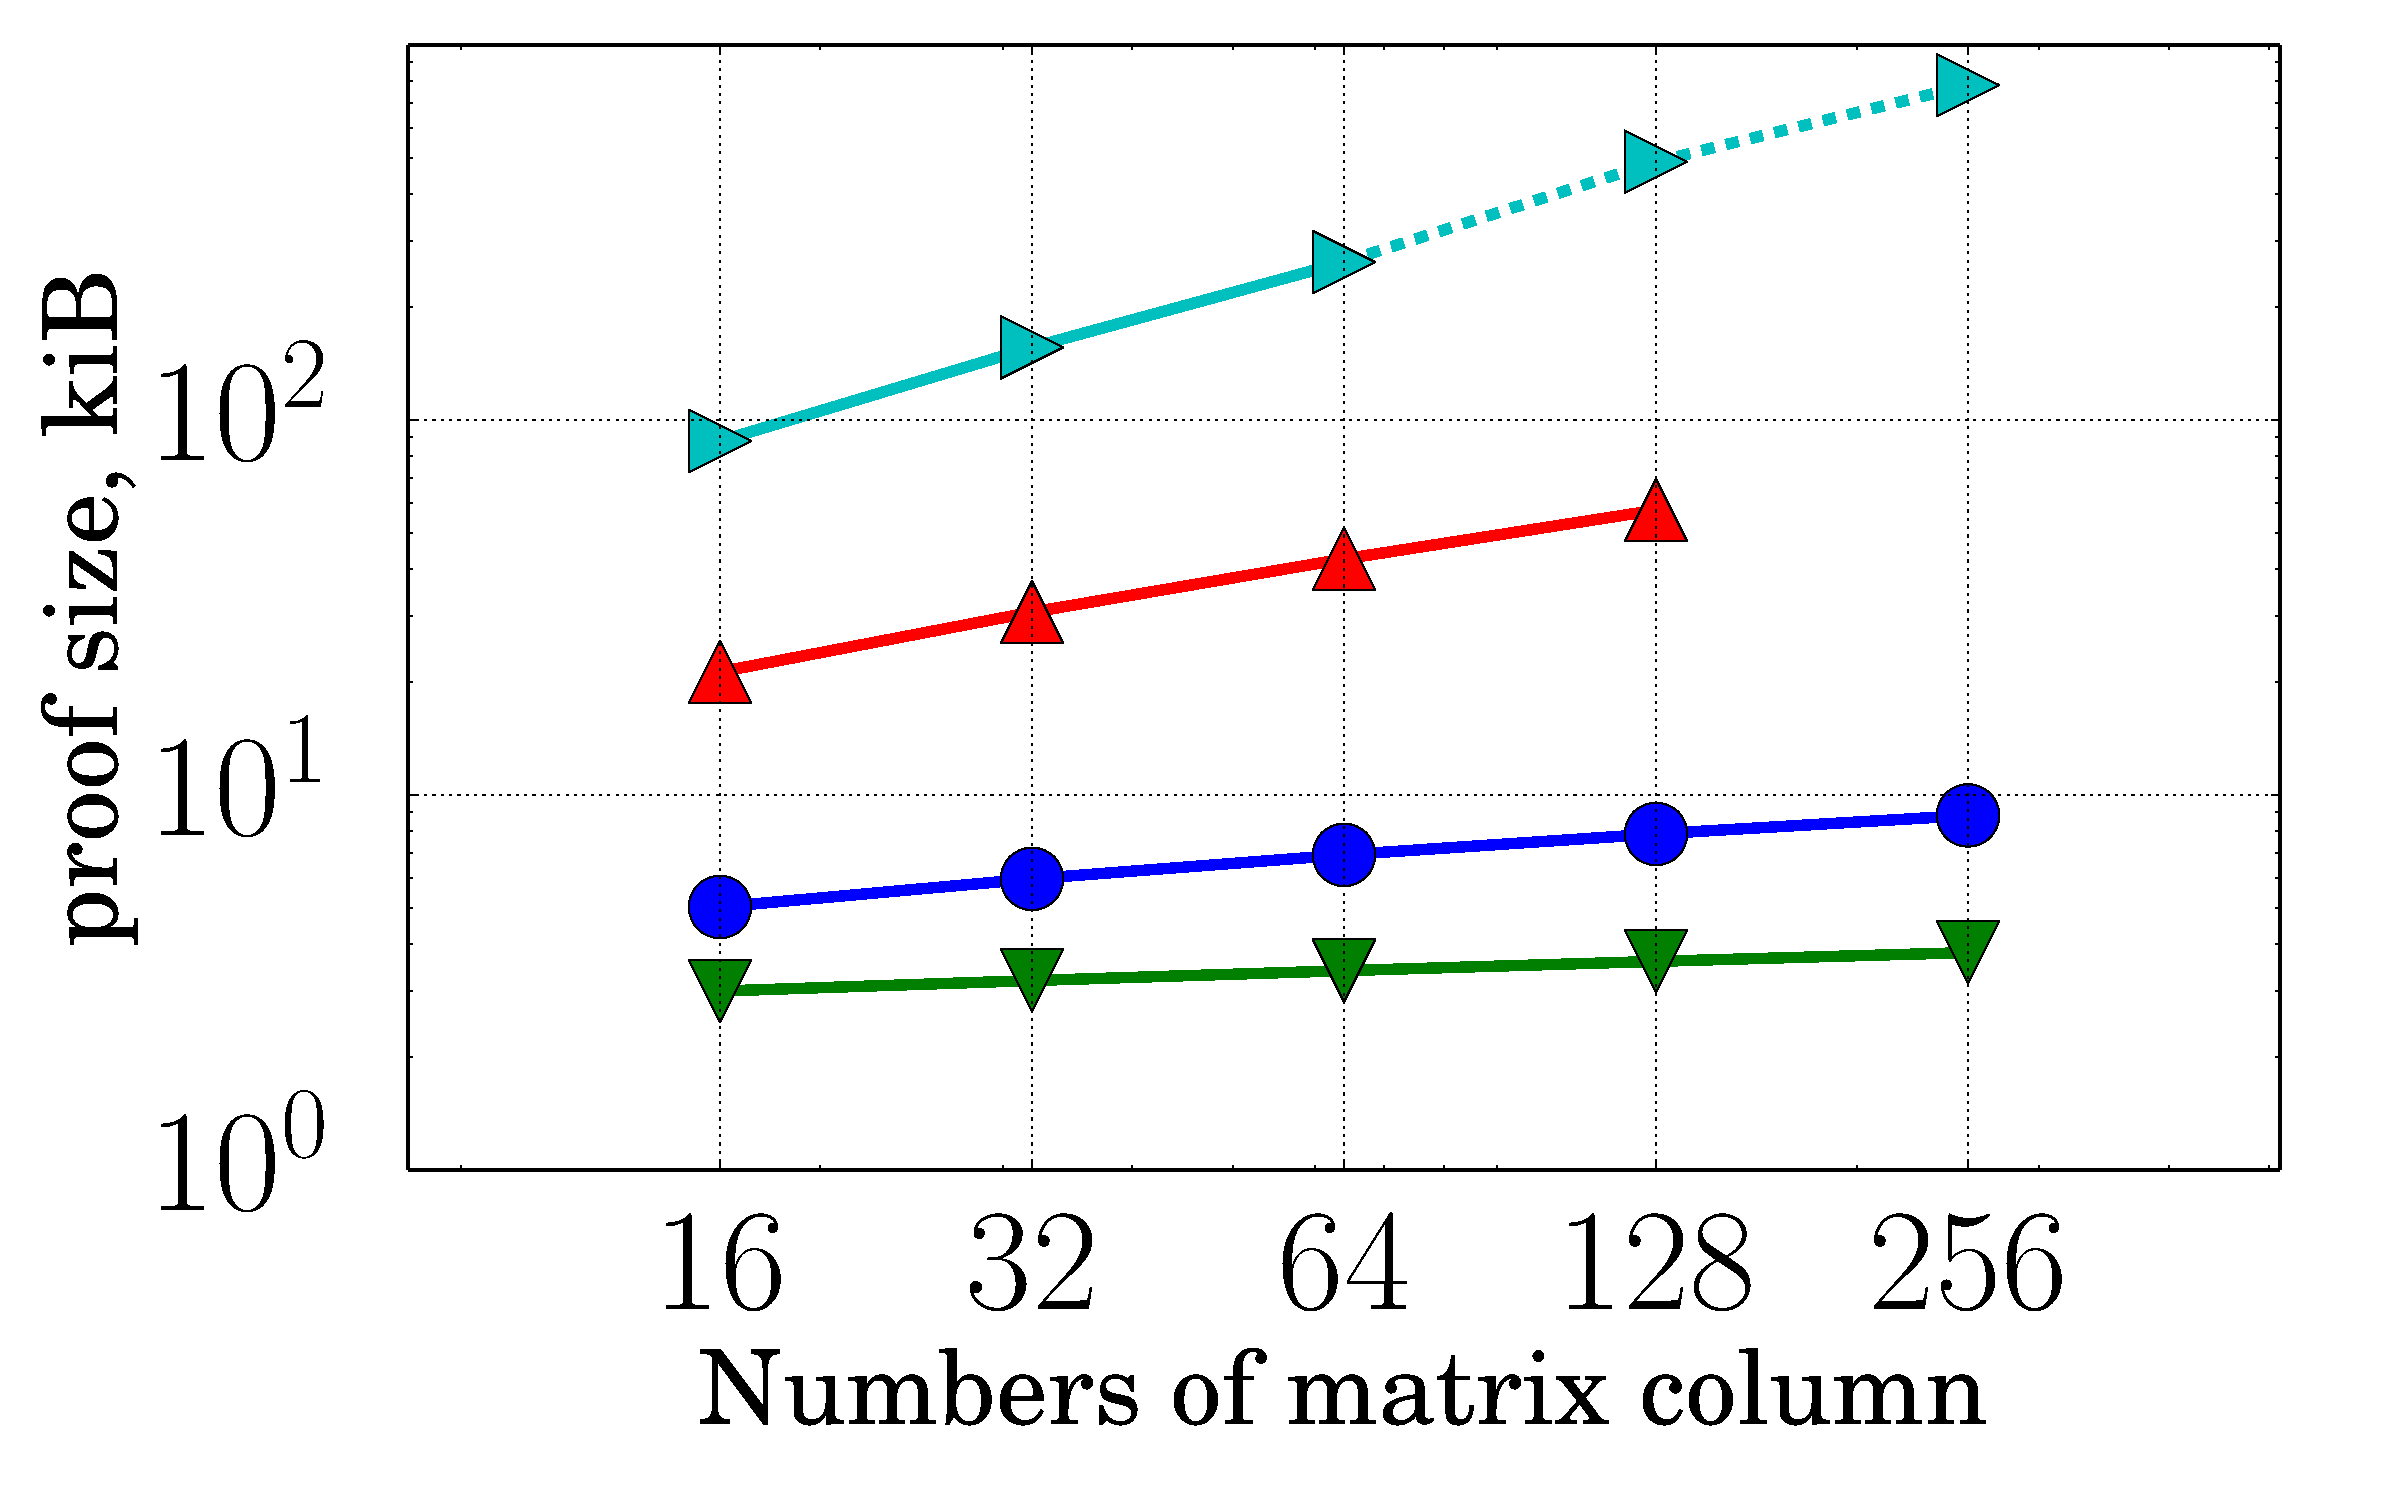
\includegraphics[width=2.1in]{fig1.pdf}
%\caption{fig1}
%\end{minipage}%
}%
%\hspace{0.05in}
\subfigure[Proof size: 16x Lanczos scaling]{
%\begin{minipage}[t]{0.25\linewidth}
%\centering
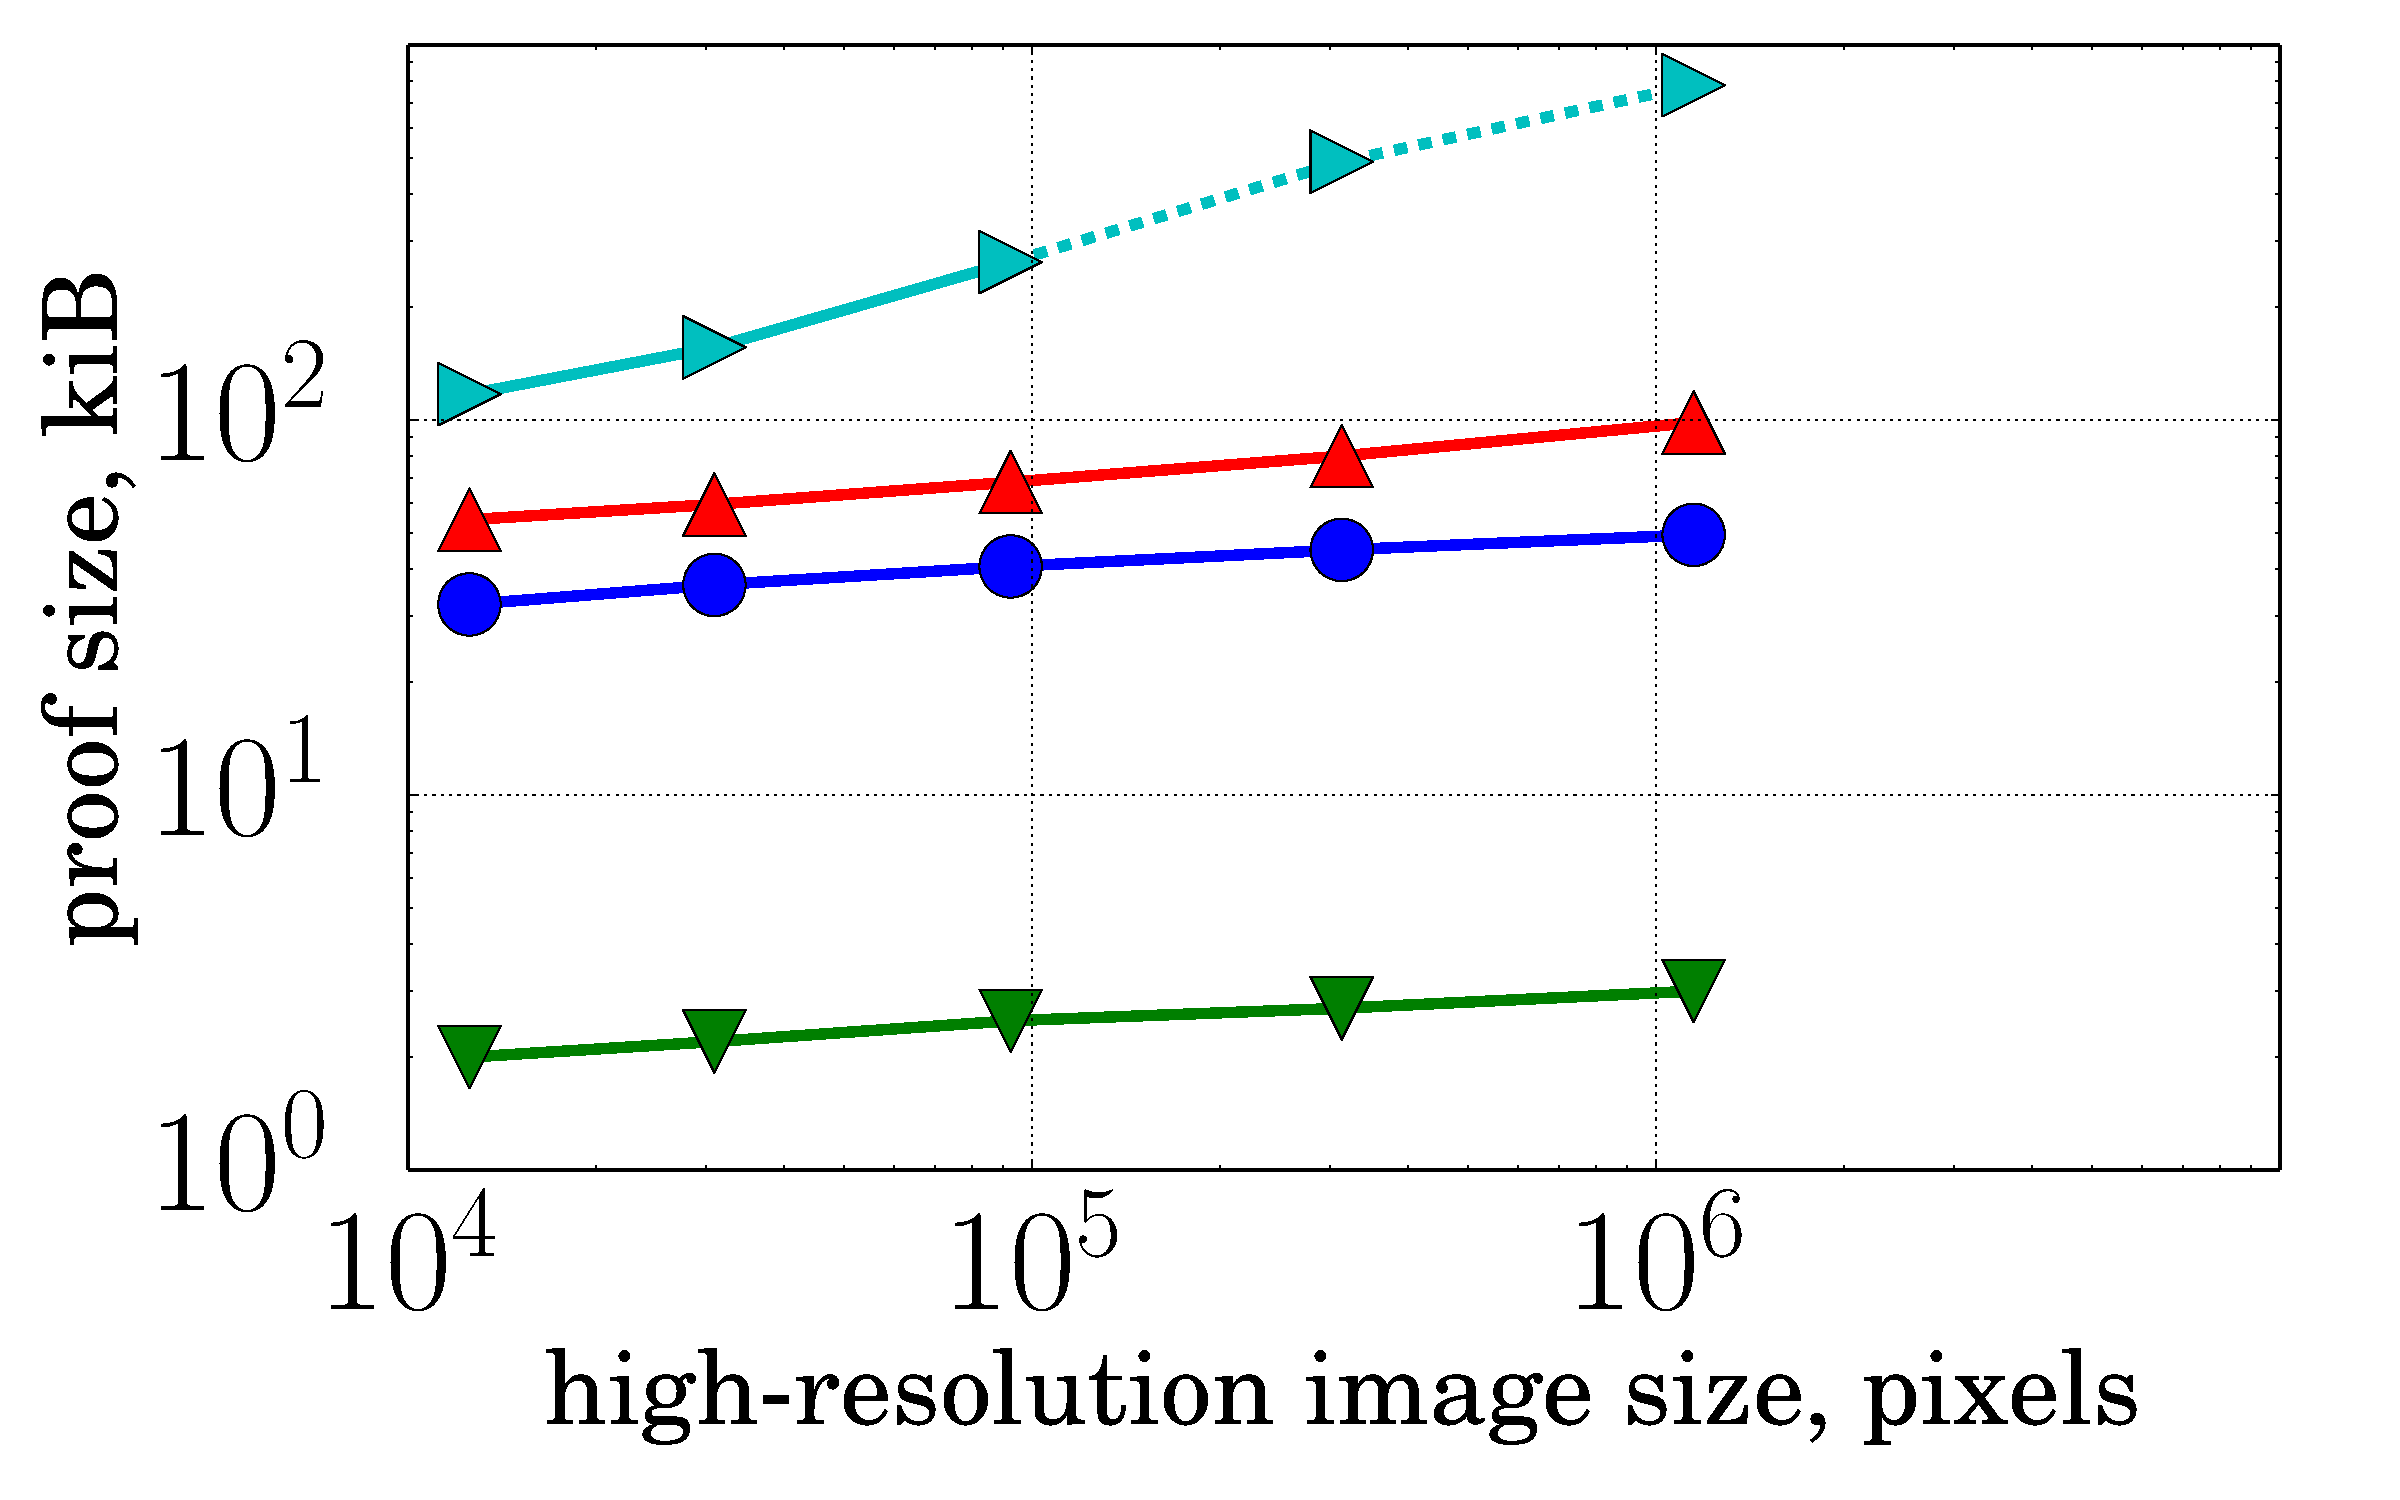
\includegraphics[width=2.1in]{fig2.pdf}
%\caption{fig2}
%\end{minipage}%
}%
%\hspace{0.05in}
\subfigure[Proof size: SHA-256 Merkle tree]{
%\begin{minipage}[t]{0.25\linewidth}
%\centering
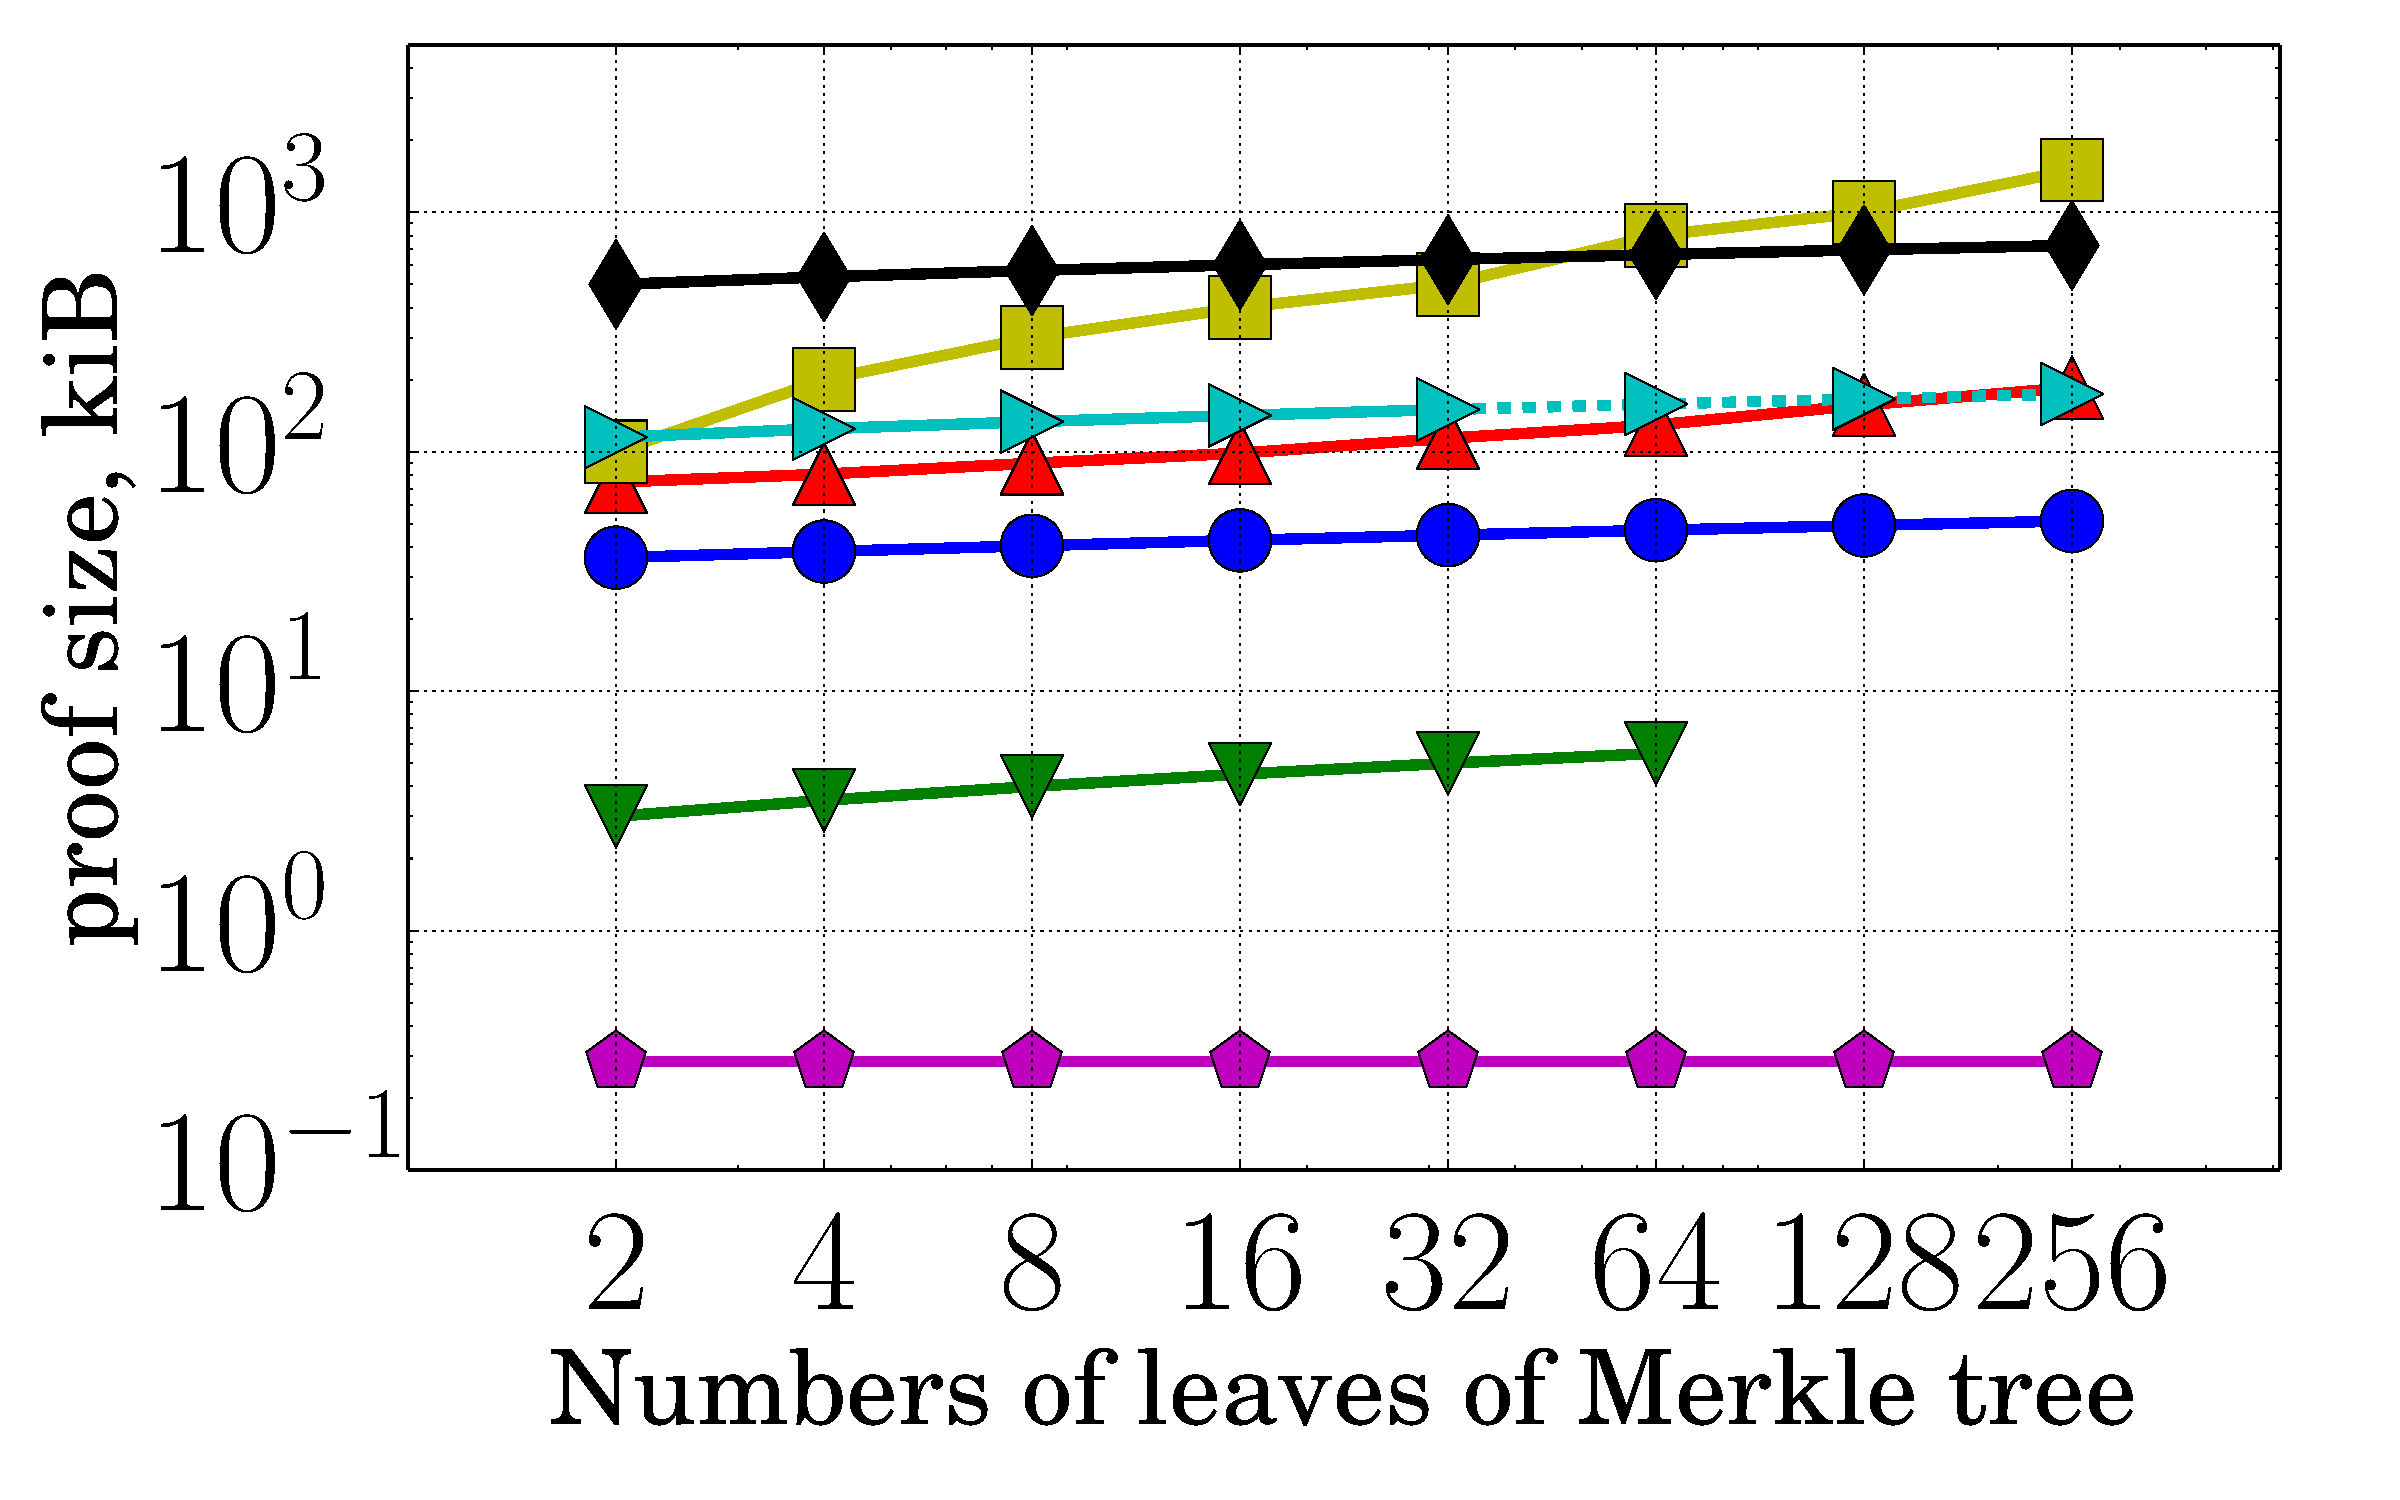
\includegraphics[width=2.1in]{fig3.pdf}
%\caption{fig2}
%\end{minipage}%
}%
\quad           
\subfigure[$\mathcal{P}$ time: 64x64 matrix multiplication]{
%\begin{minipage}[t]{0.25\linewidth}
%\centering
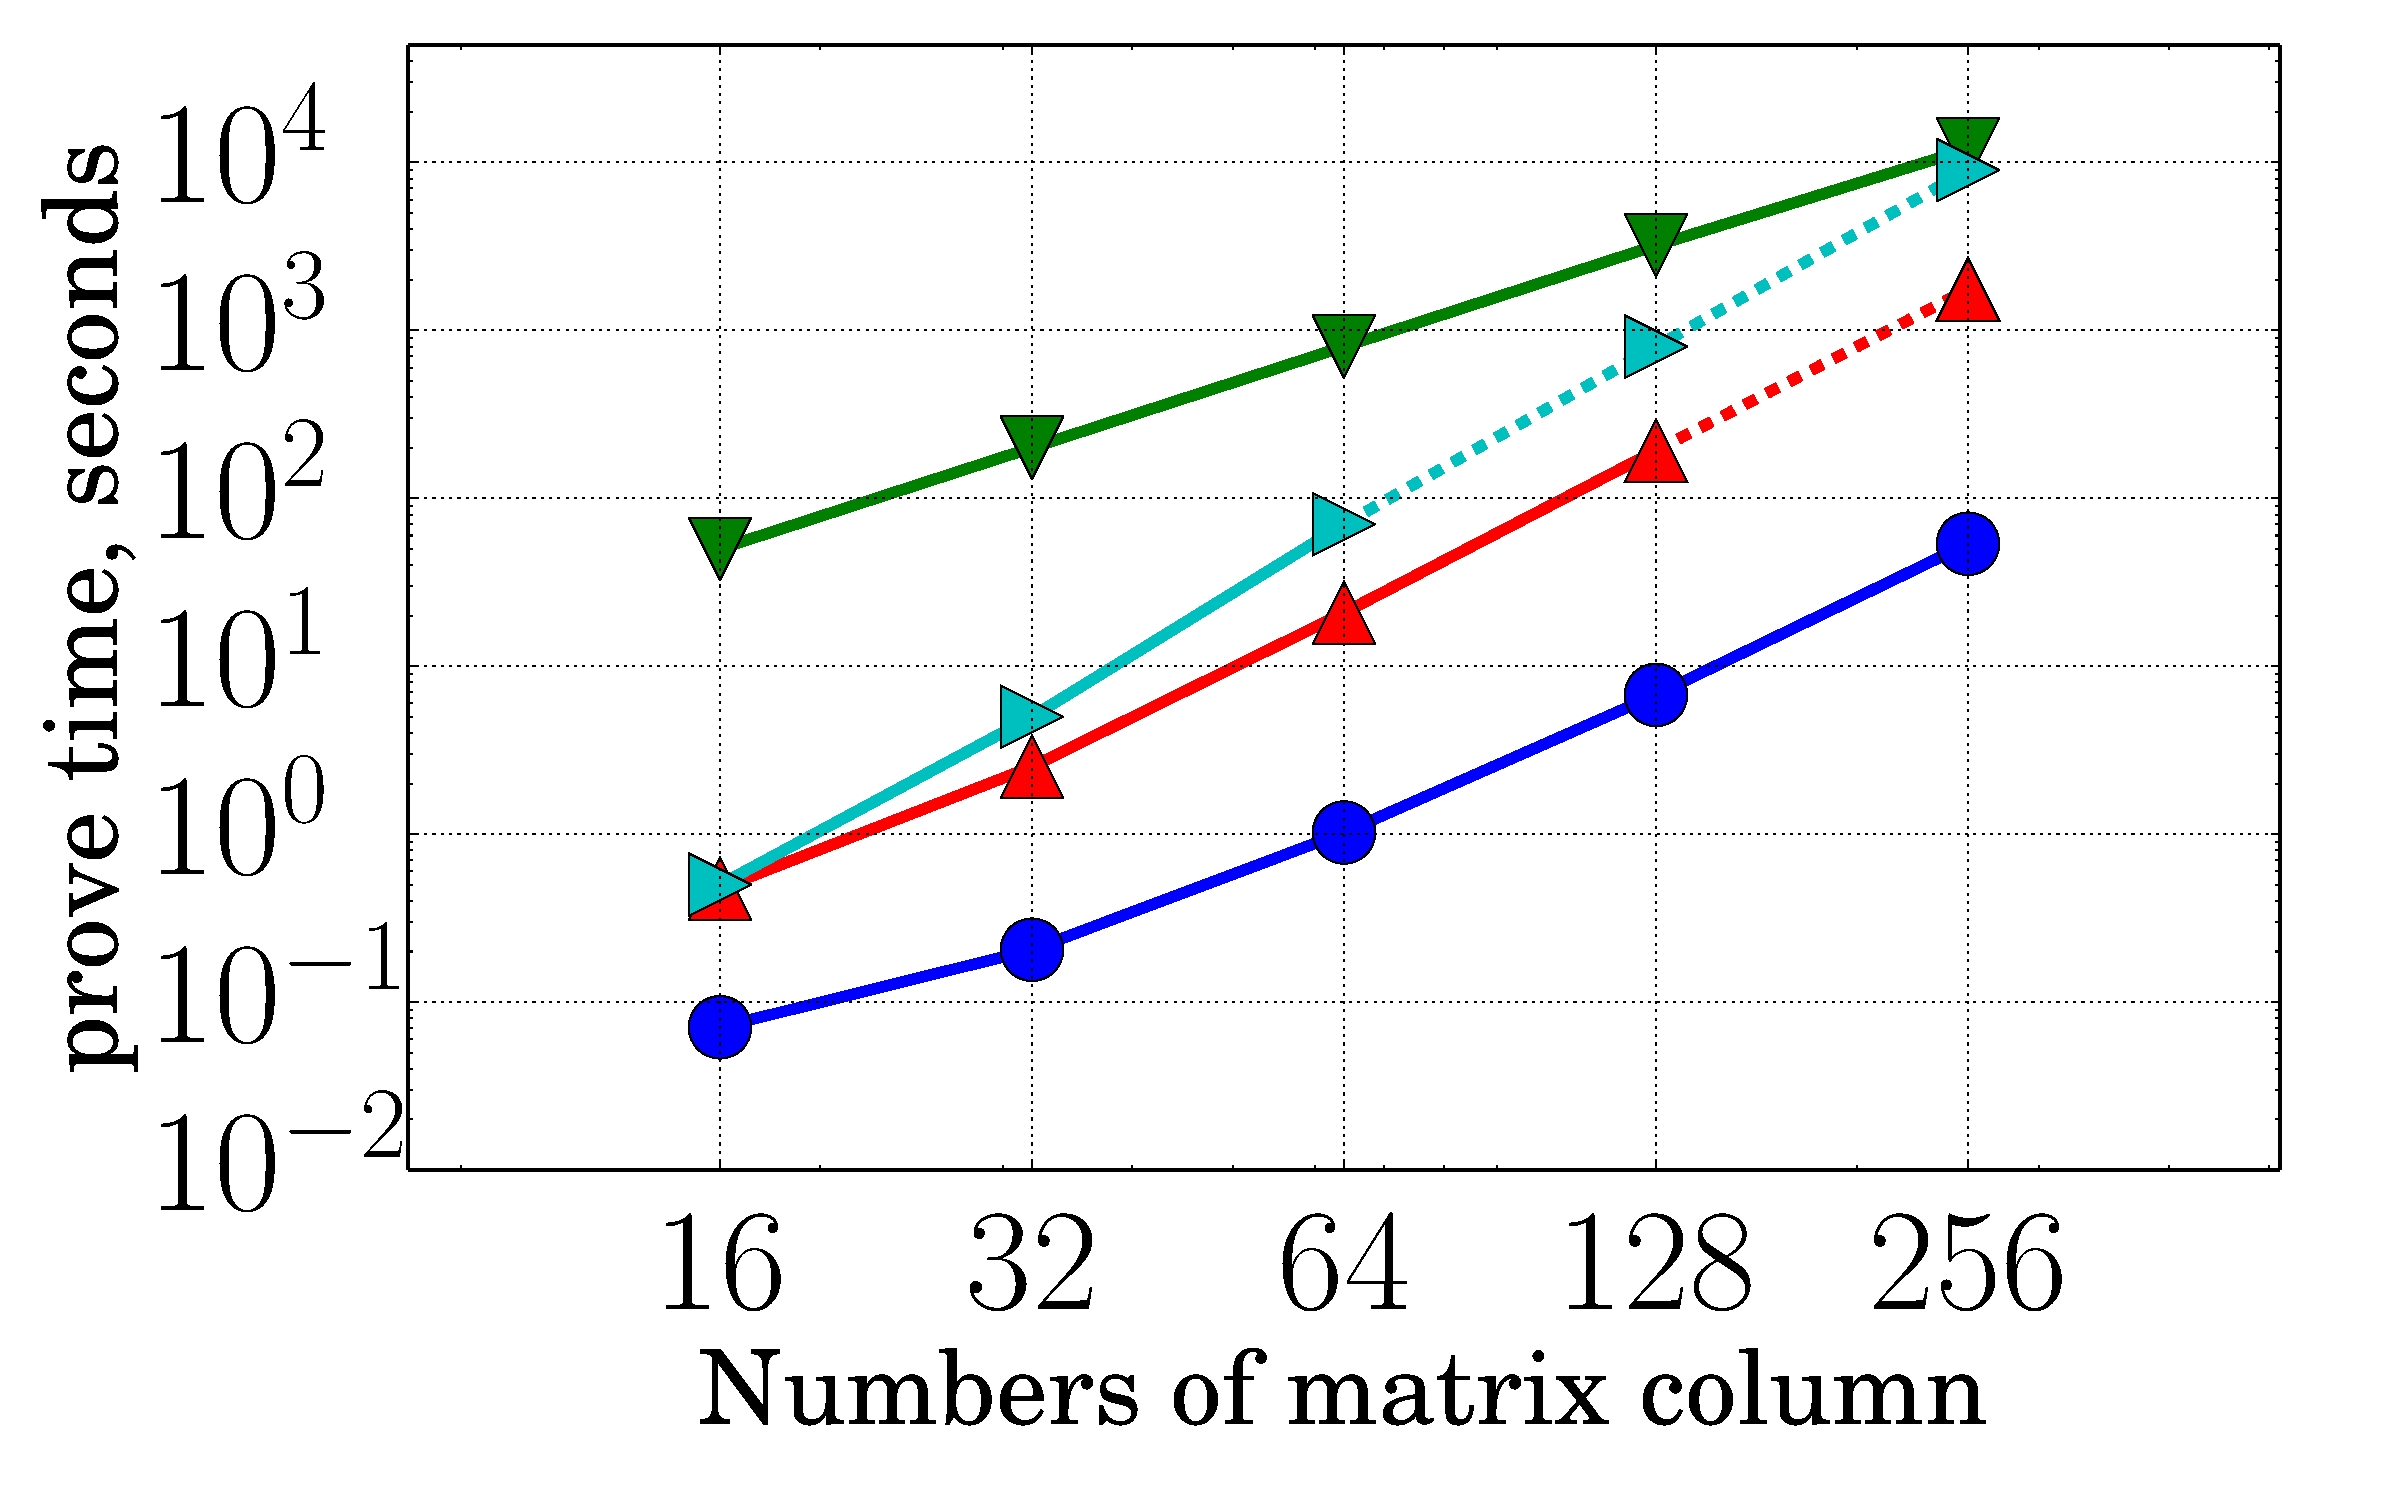
\includegraphics[width=2.1in]{fig4.pdf}
%\caption{fig2}
%\end{minipage}
}%
%\hspace{0.65in}
\subfigure[$\mathcal{P}$ time: 16x Lanczos scaling]{
%\begin{minipage}[t]{0.25\linewidth}
%\centering
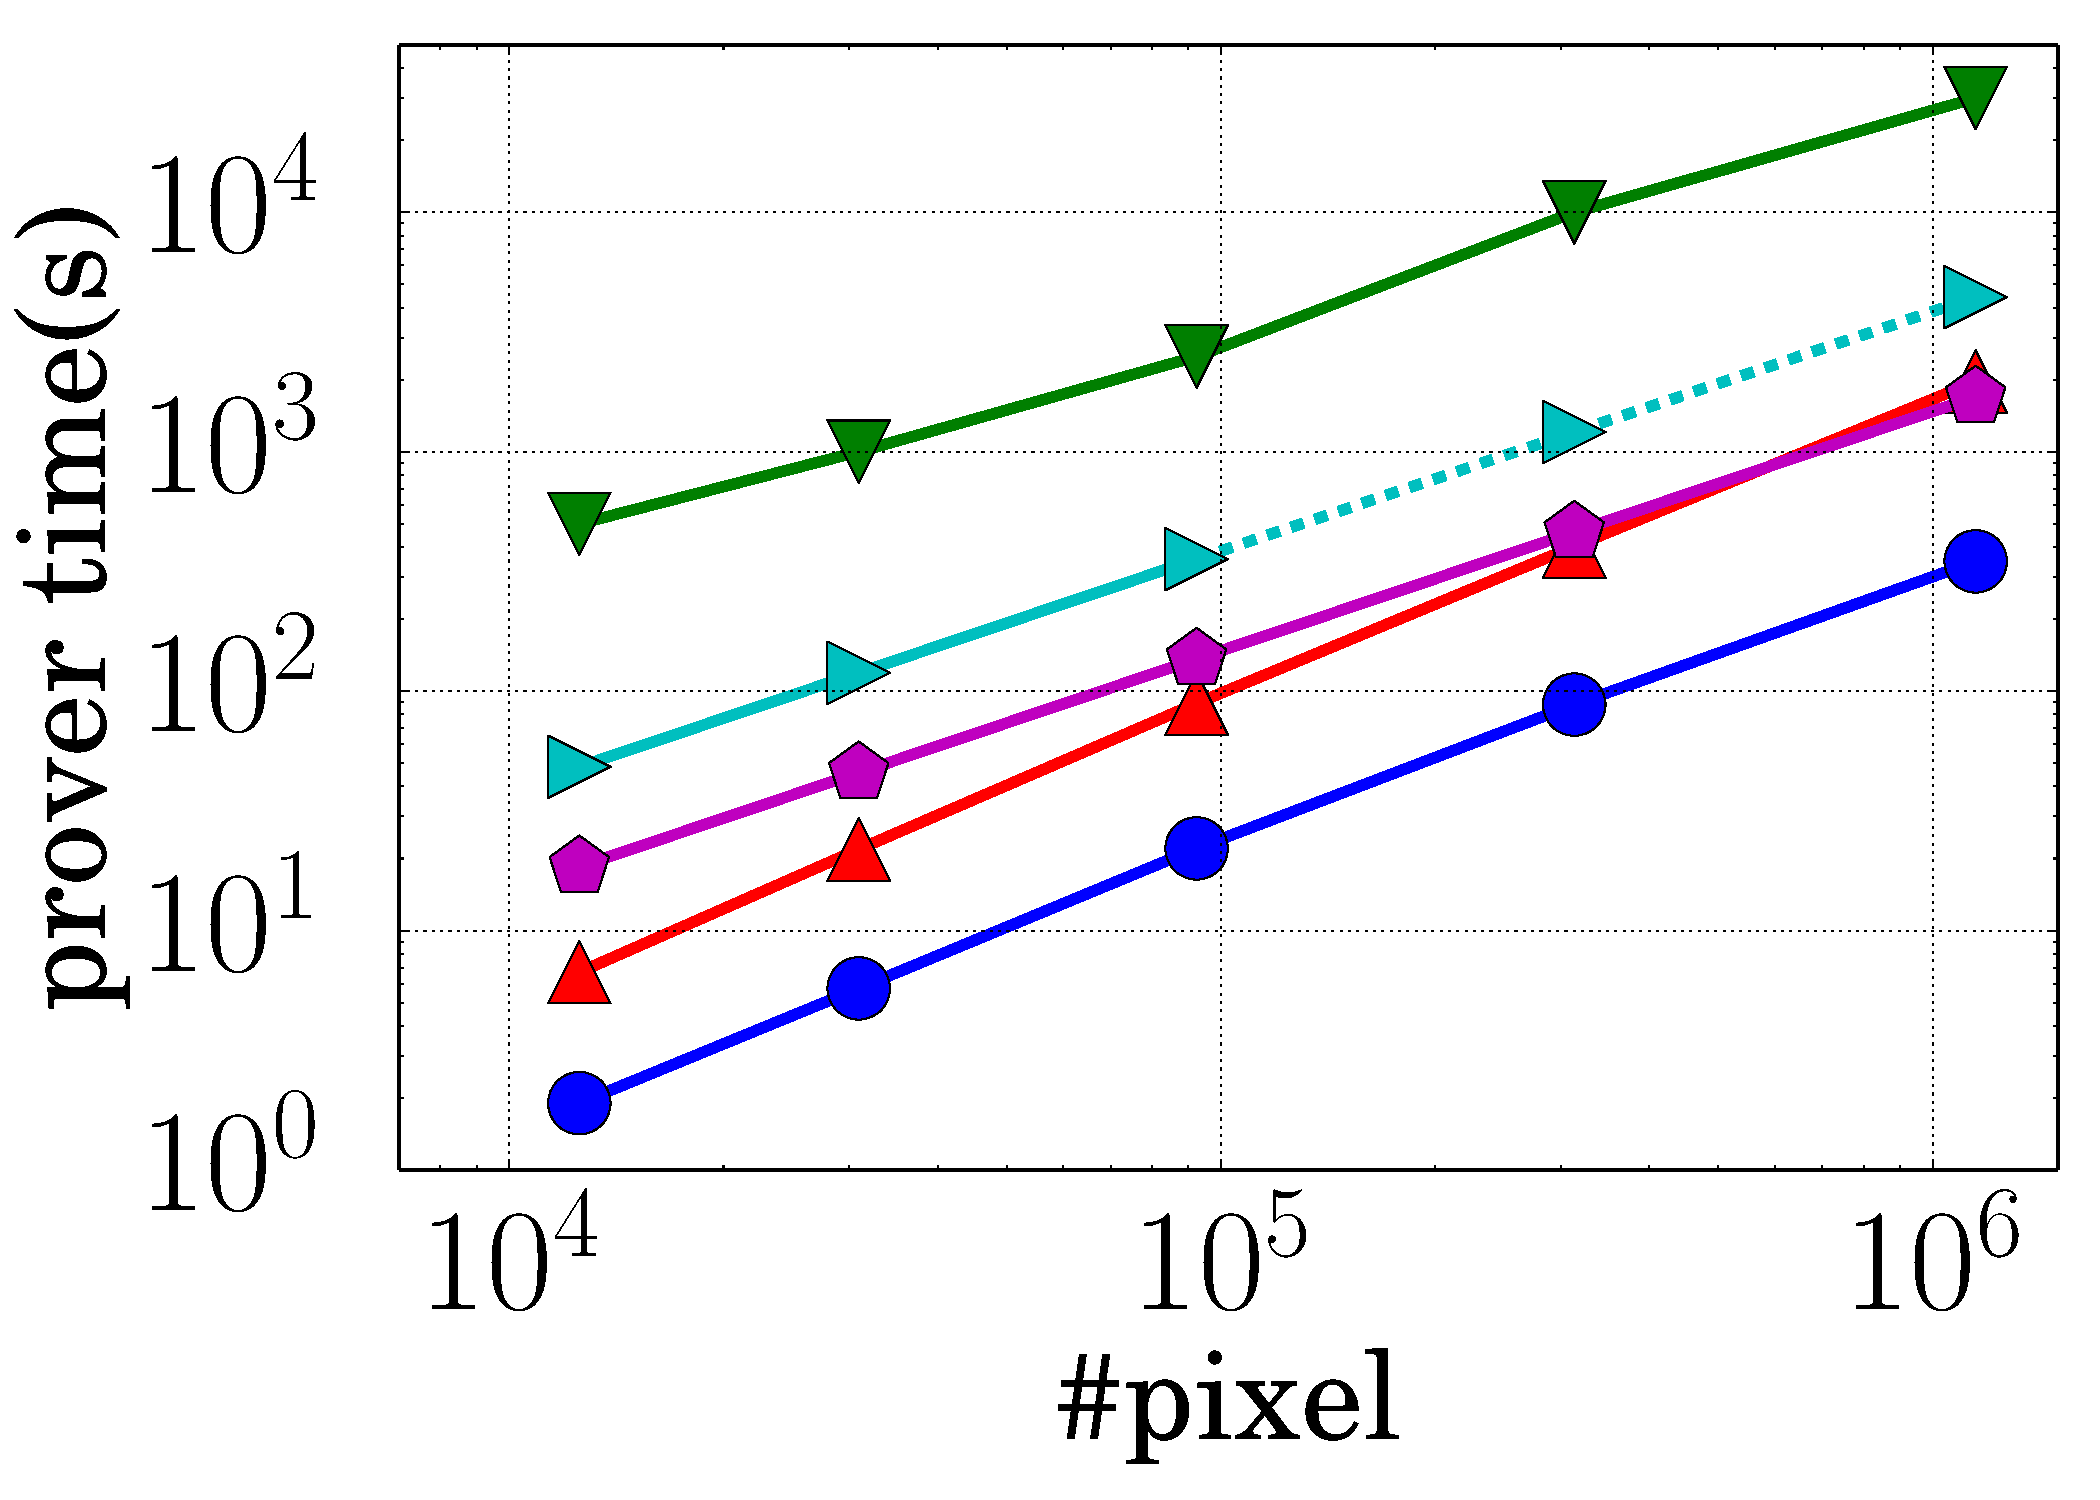
\includegraphics[width=2.1in]{fig5.pdf}
%\caption{fig2}`
%\end{minipage}
}%
%\hspace{0.65in}
\subfigure[$\mathcal{P}$ time: SHA-256 Merkle tree]{
%\begin{minipage}[t]{0.25\linewidth}
%\centering
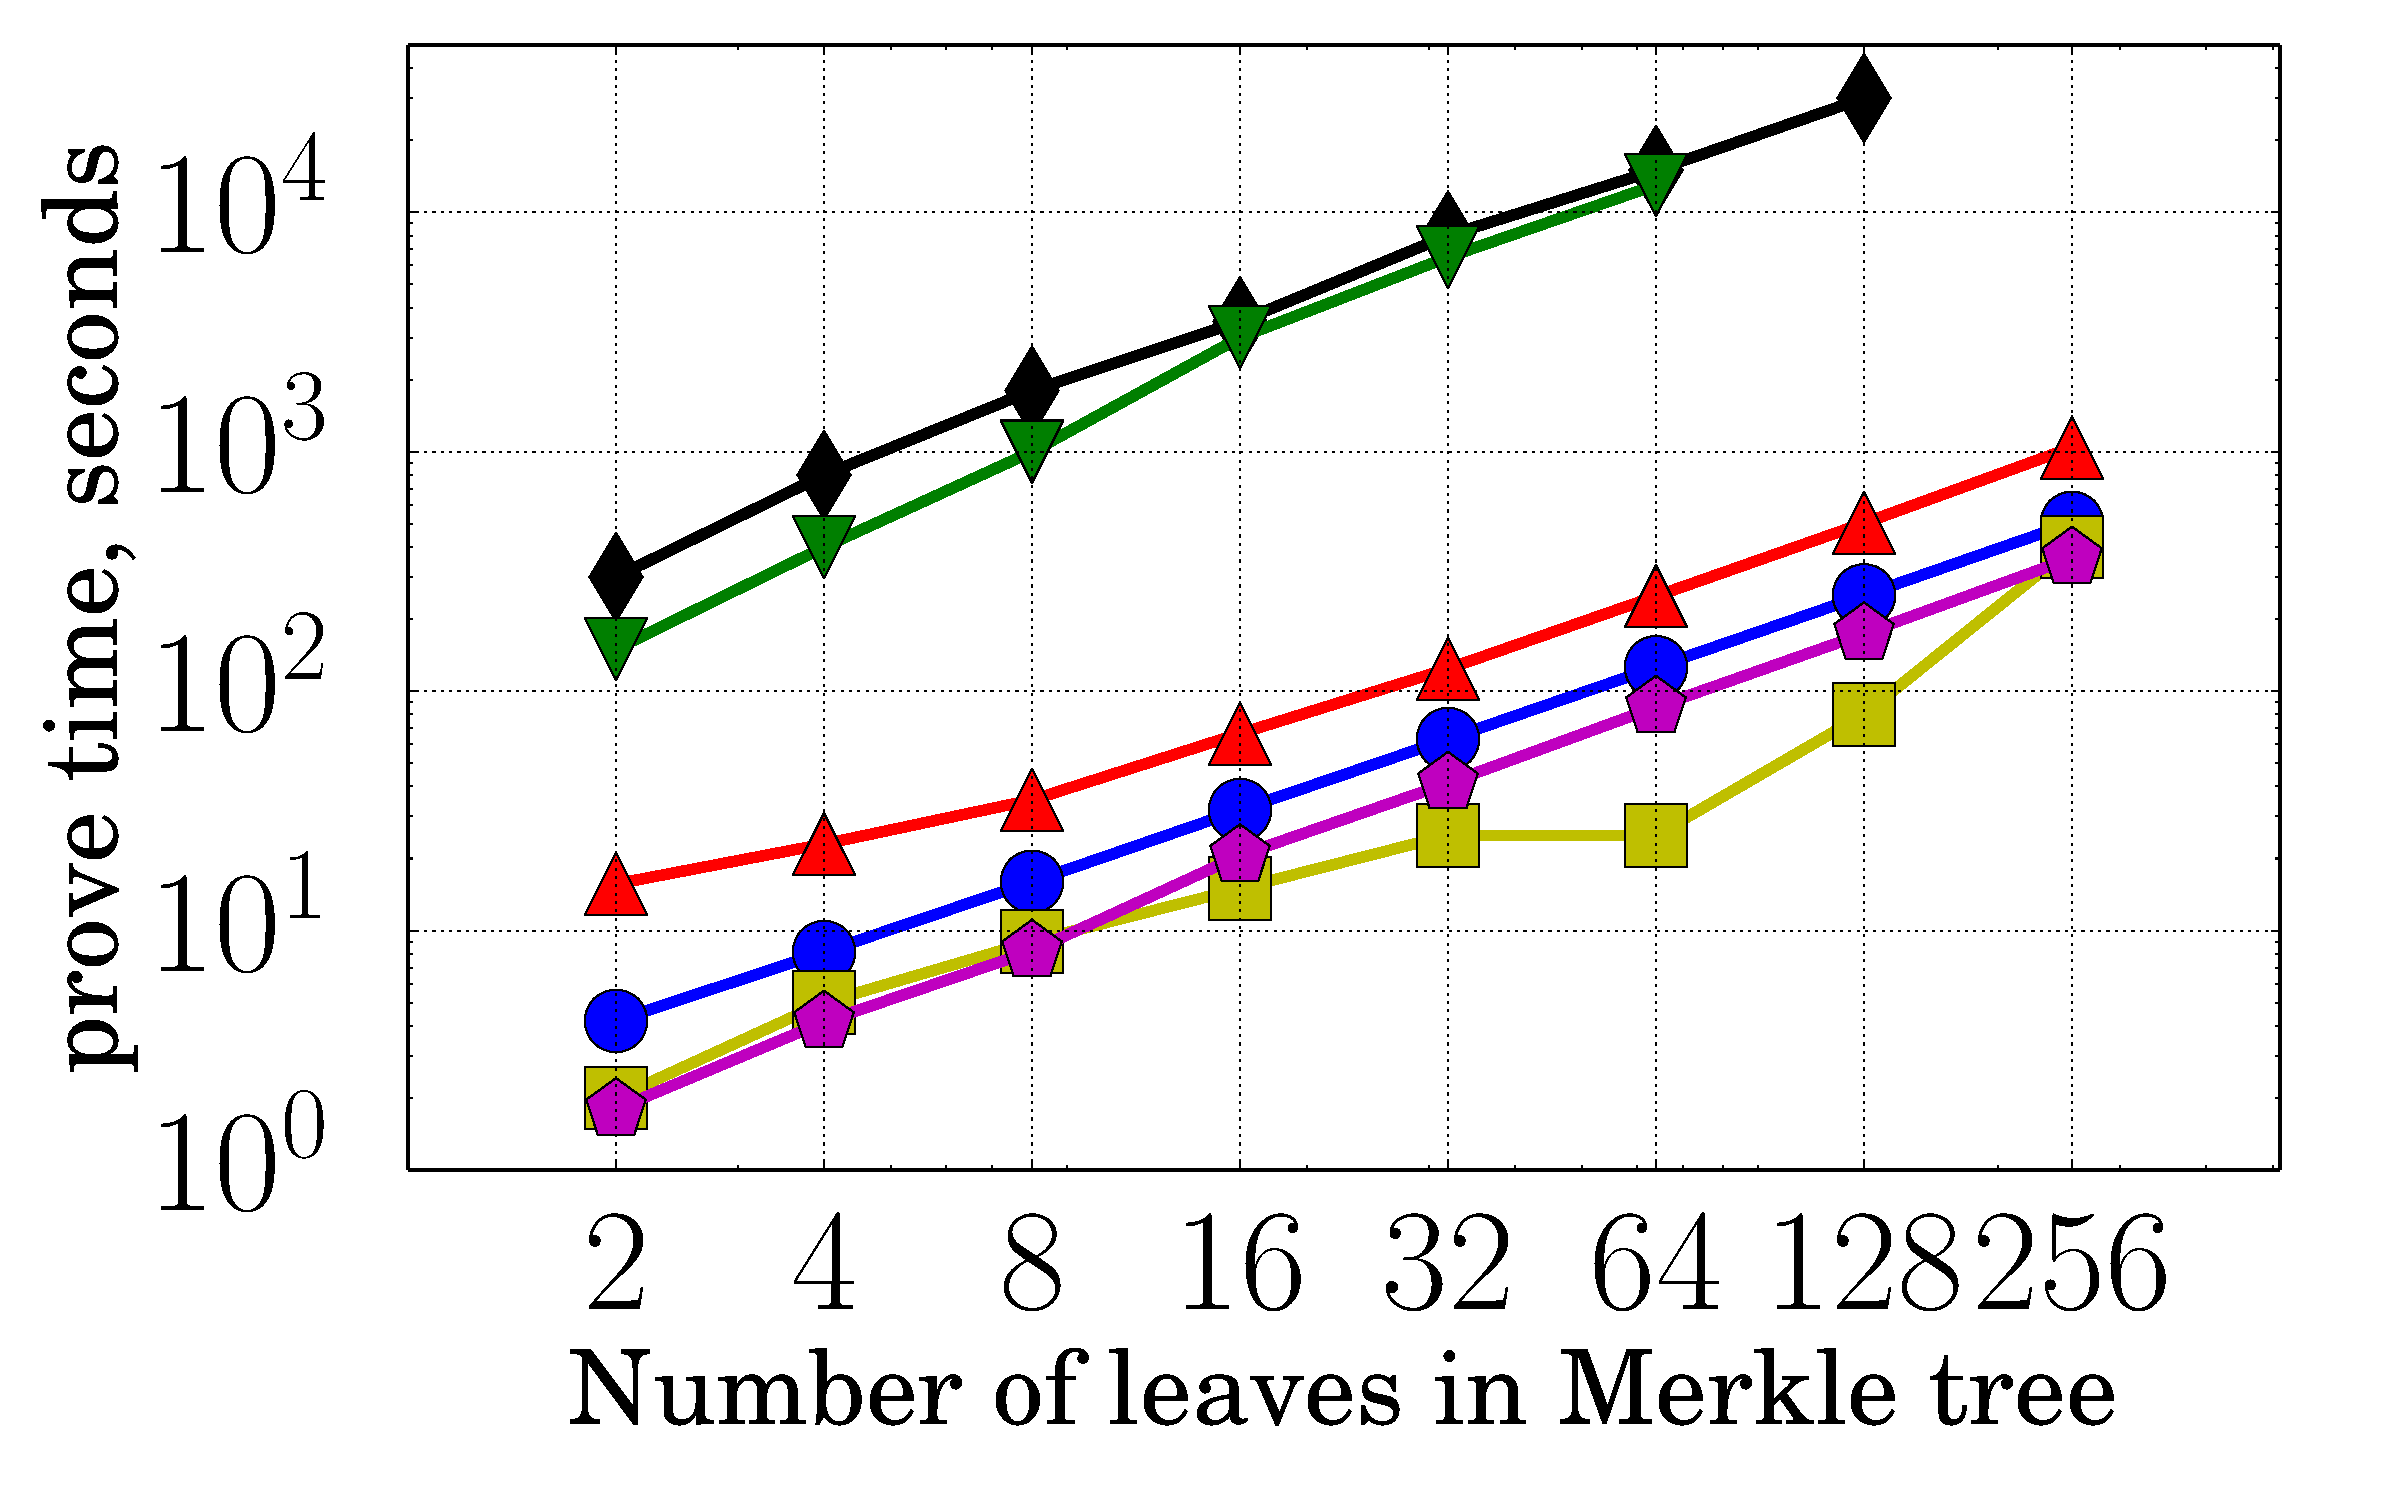
\includegraphics[width=2.1in]{fig6.pdf}
%\caption{fig2}`
%\end{minipage}
}%
\quad           
\subfigure[$\mathcal{V}$ time: 64x64 matrix multiplication]{
%\begin{minipage}[t]{0.25\linewidth}
%\centering
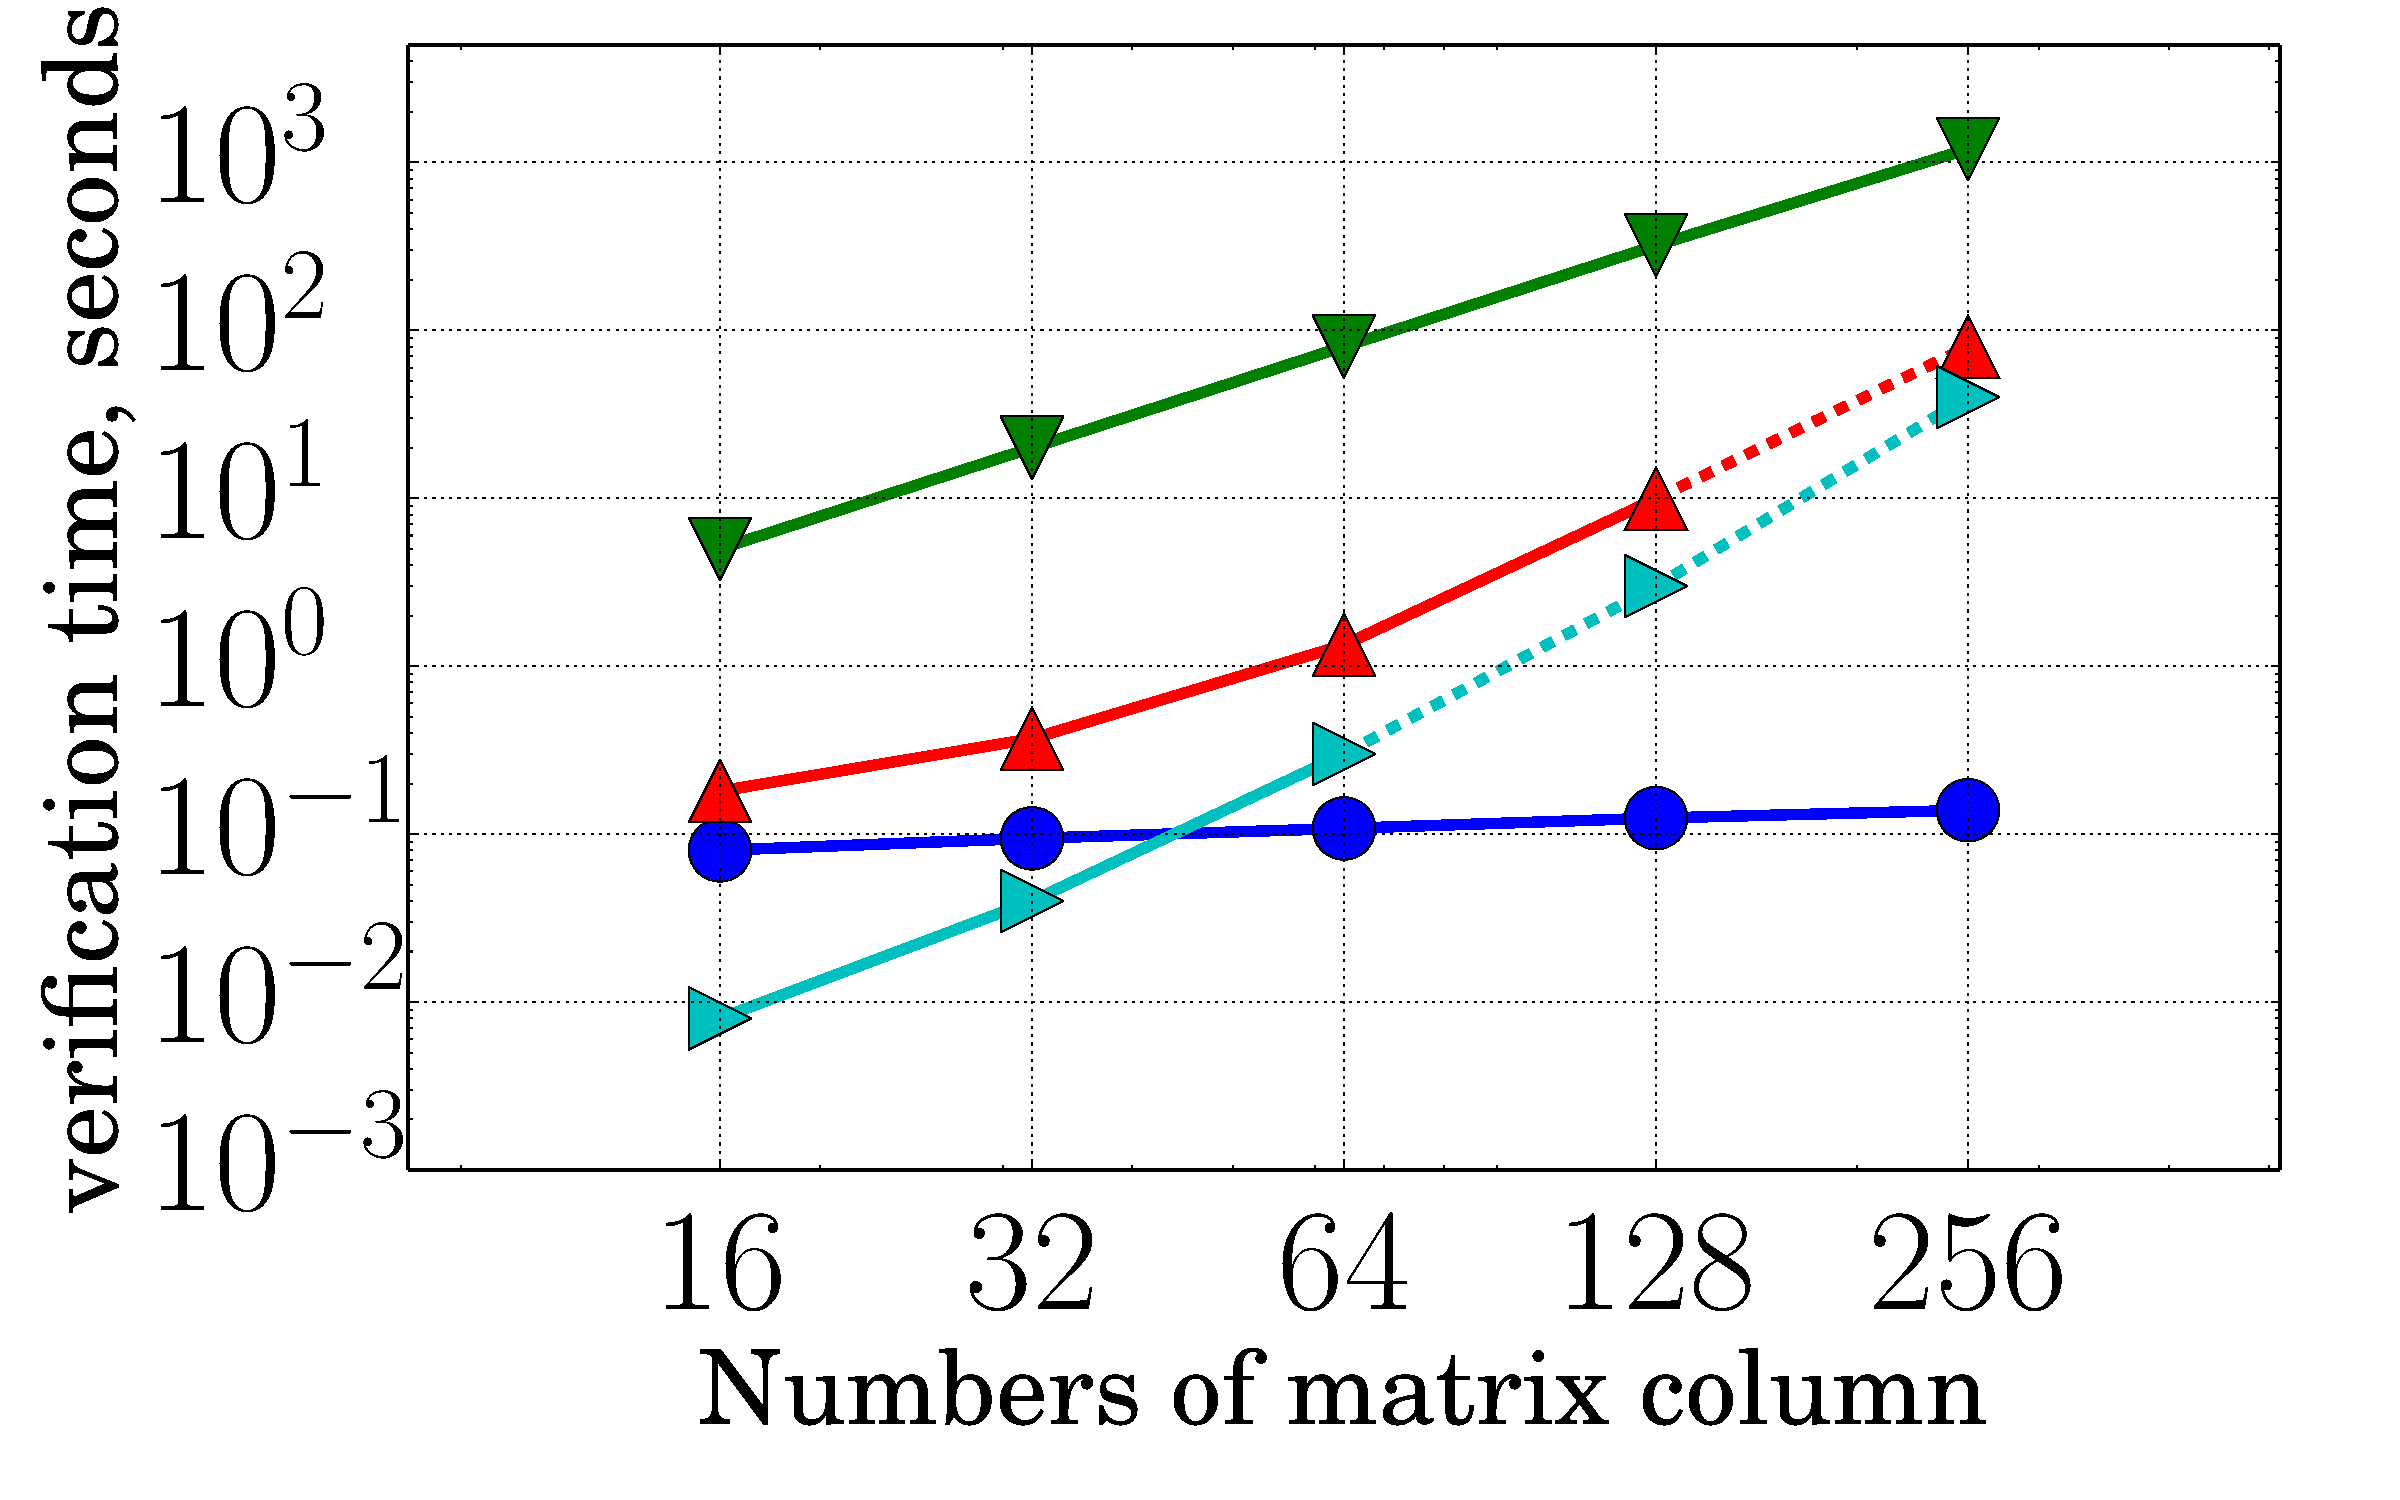
\includegraphics[width=2.1in]{fig7.pdf}
%\caption{fig2}
%\end{minipage}
}%
%\hspace{0.65in}
\subfigure[$\mathcal{V}$ time:16x Lanczos scaling]{
%\begin{minipage}[t]{0.25\linewidth}
%\centering
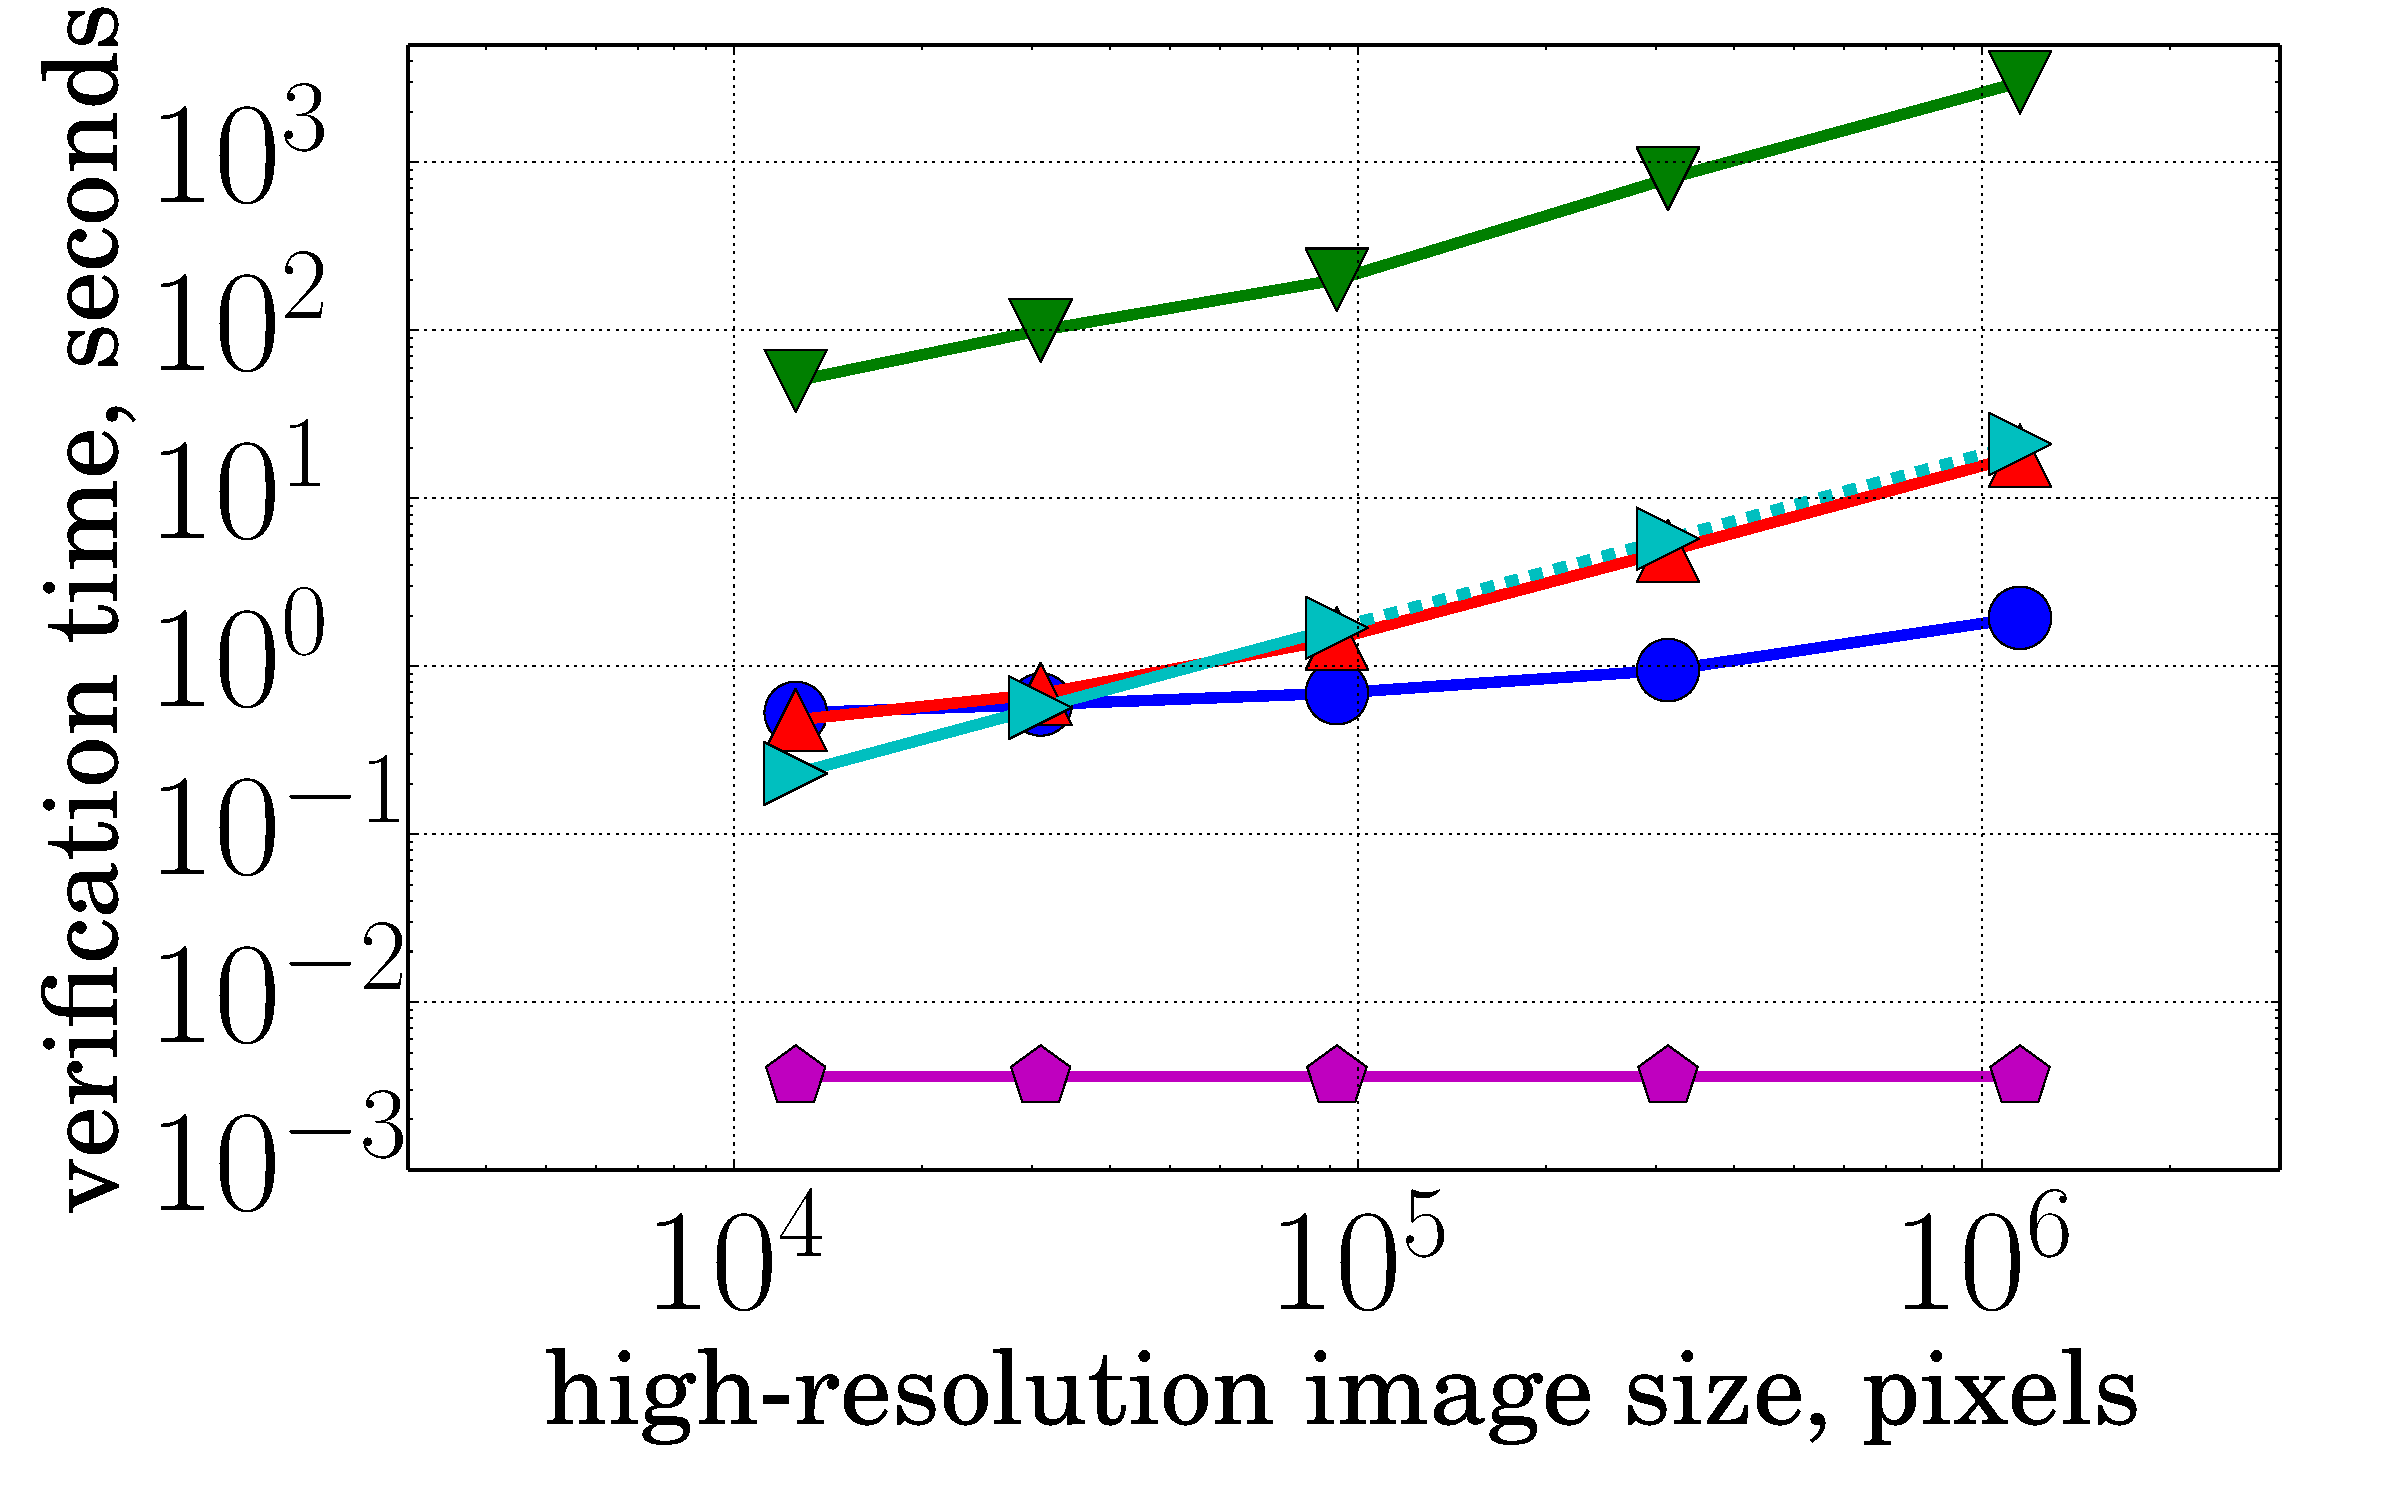
\includegraphics[width=2.1in]{fig8.pdf}
%\caption{fig2}`
%\end{minipage}
}%
%\hspace{0.65in}
\subfigure[$\mathcal{V}$ time:SHA-256 Merkle tree]{
%\begin{minipage}[t]{0.25\linewidth}
%\centering
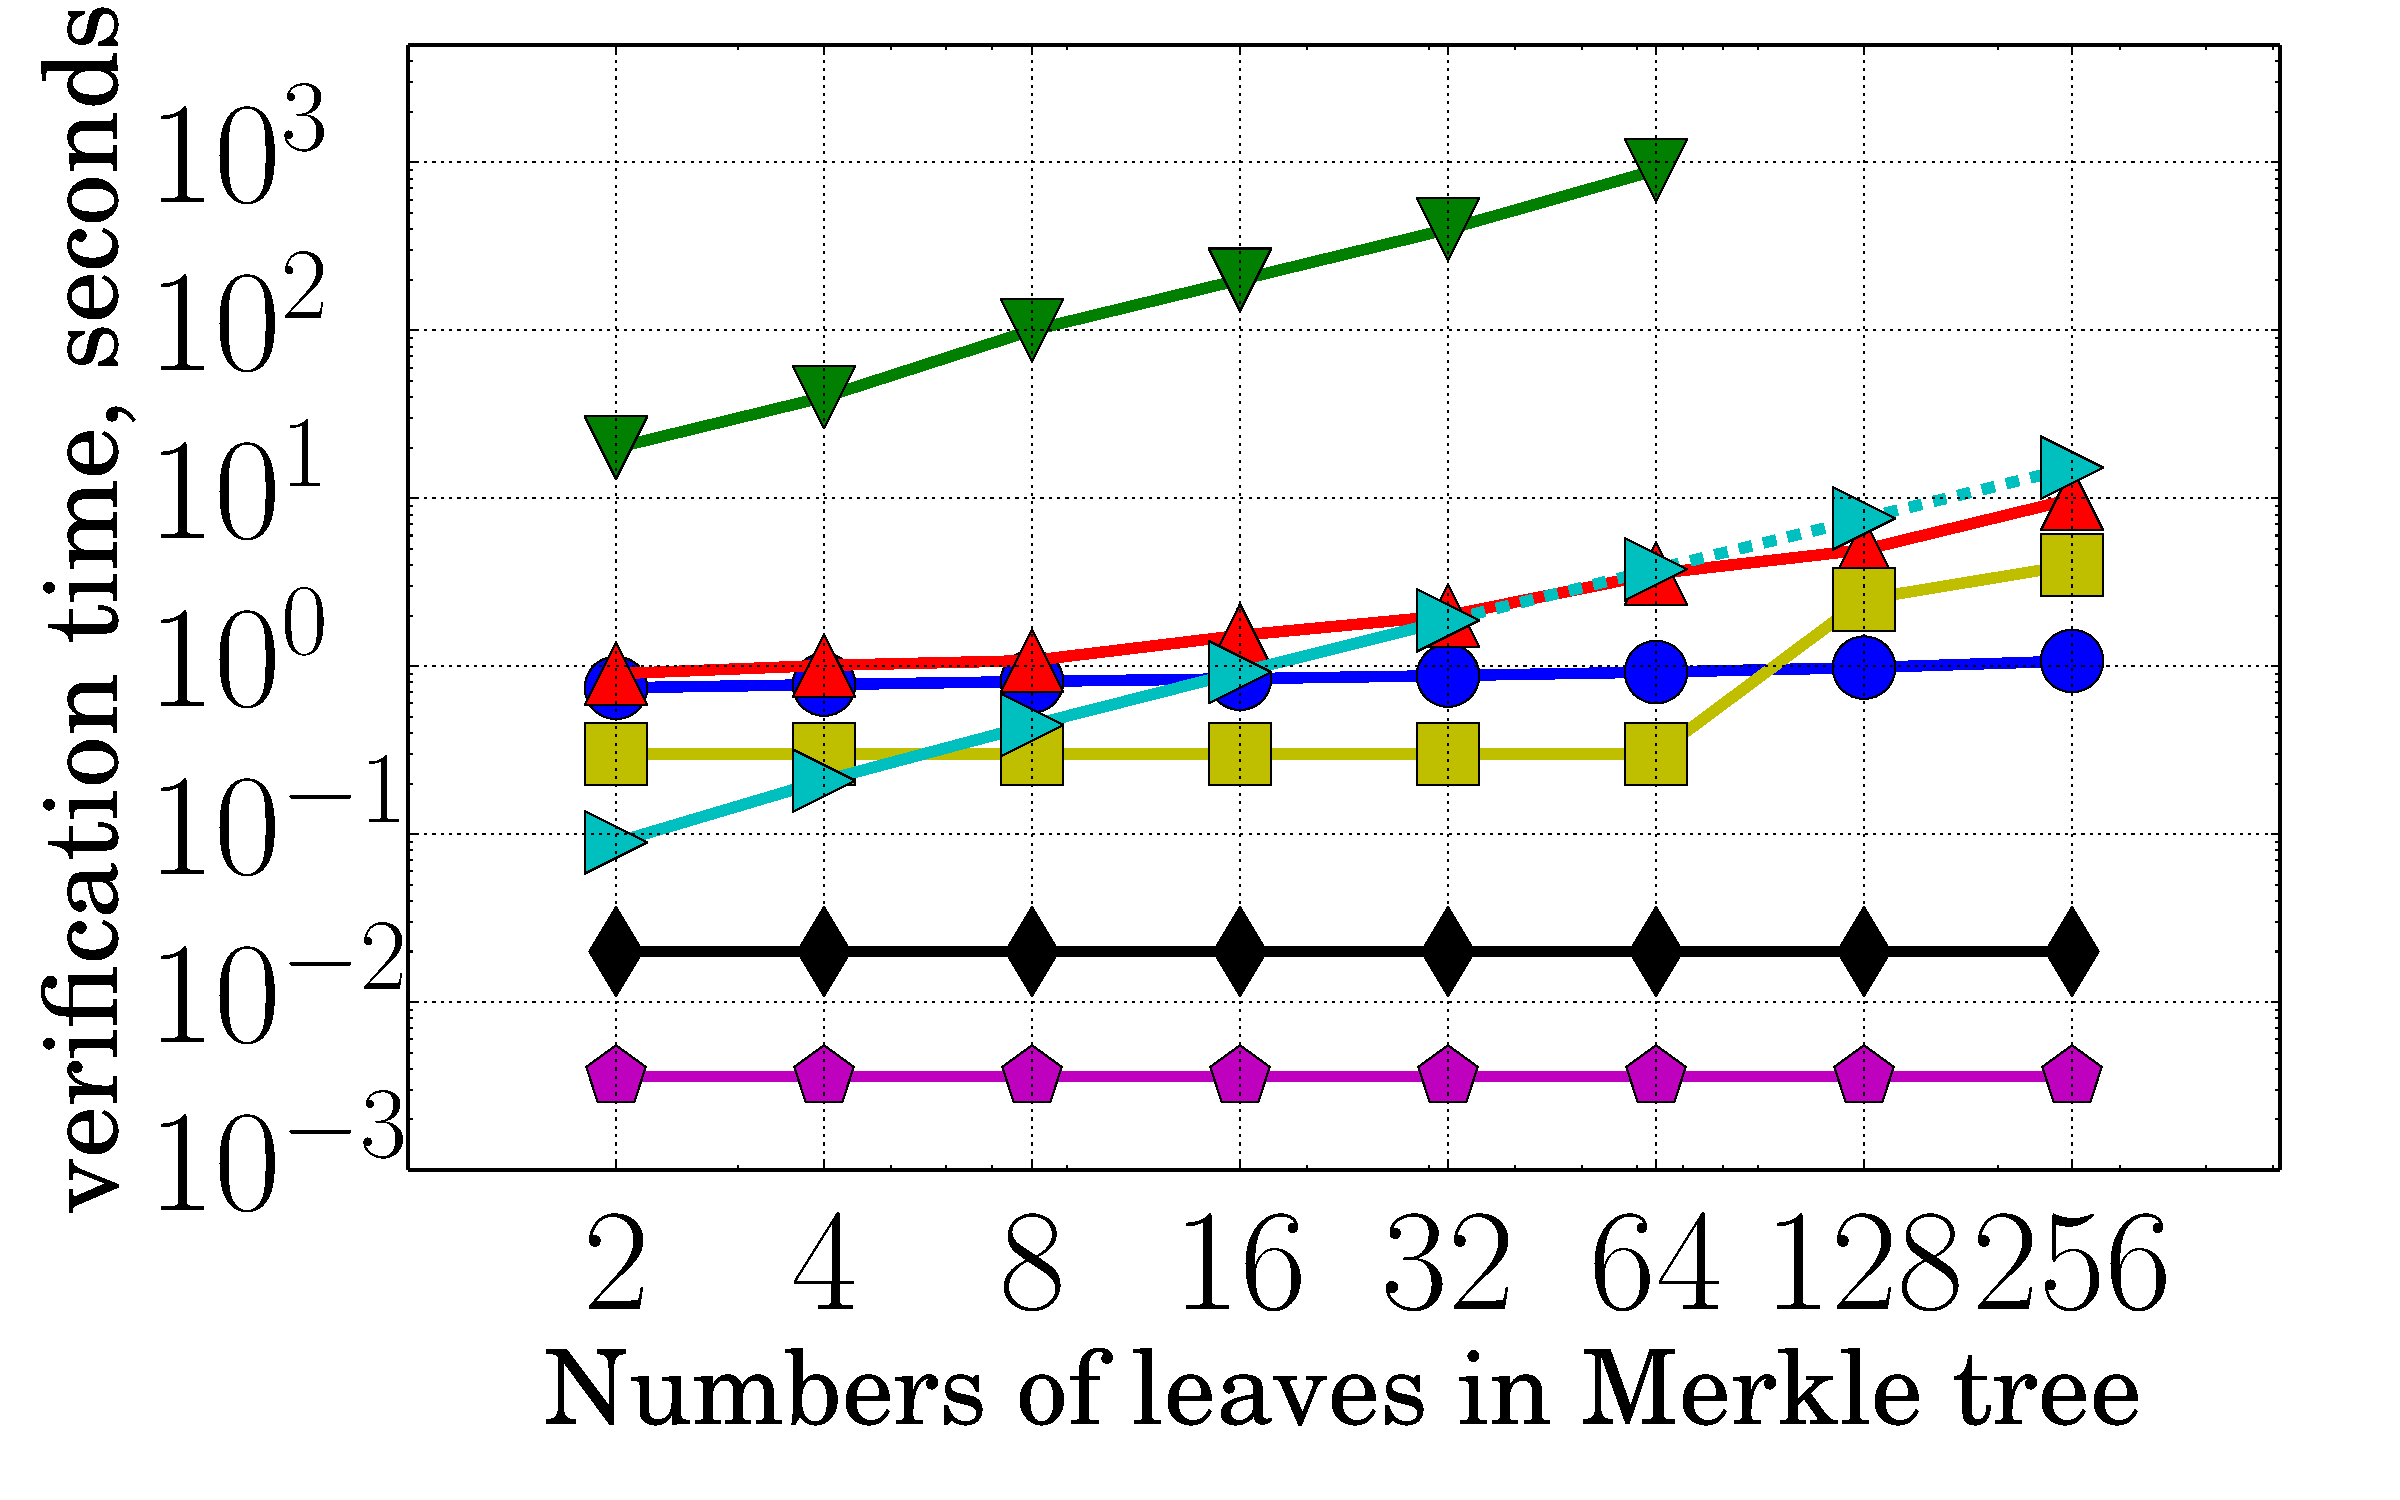
\includegraphics[width=2.1in]{fig9.pdf}
%\caption{fig2}`
%\end{minipage}
}%
%\centering
\quad
\centering

\includegraphics[width = 6.5in]{legend.pdf}
\caption{\label{fig:Allcom}Comparisons of prover time, proof size and verification time between \name{} and existing zero knowledge proof systems.}
\end{figure}

\paragraph{Experimental results.} All of experimental results are summarized in Figure \ref{ZKGKR}. We would analyse the consequences from four perspectives: prove time, verification time, proof size and memory consumption.
\begin{itemize}
	\item \textbf{prove time}: Generally, the prove time of \name{} is comparable with Ligero and much faster than any other systems. That is because Ligero is not based on the public key cryptography. For instance, for matrix multiplication, when the matrix size is 128x128, our system's prove time is roughly 5x speed up of Hyrax, 100x speed up of libSTARK and only a little slower than Ligero. For image scaling, when the number of pixels are 1072x1072, our system is...
	\item \textbf{verification time}: Generally, the verification time of \name{} is faster all other systems except libSTANK and lib SNARK. The reason is that the verifiers in libSTANK and libSNARK only have constant cost. For Merkle tree, when the leaves of Merkle tree is 256, our verification time is 3x faster than Hyrax and 2x faster than but libSTARK remains the constant. 
	\item \textbf{proof size}: For proof size, our system is smaller than other systems except for Bulletproofs since the proof size of Bulletproofs is constant while ours is logarithmic. For Merkel tree, when the number of leaves are 256, Hyrax's proof size is about 5x larger than ours while libSTARK's proof size is 10x larger than ours, but Bulletproofs' proof size remains constant.  
	\item \textbf{memory consumption}: LibSTARK, libSNARK and Bulletproofs are all high memory consumed. They run out of RAM for the medium size of the test data for matrix multiplication and Merkle tree. Our system is comparable with Hyrax and Ligero.
\end{itemize}

\subsection{Discussions}\label{subsec::discuss}

In this section, we discuss some potential improvements for \name.


\paragraph{Improving verification time.} As shown in the experiments above, the verification time in \name is already fast in practice compared to other systems, yet it can be further improved by 1-2 orders of magnitude. 

Within the verification of \name, most of the time (more than 95\% in the evaluations above) is spent on our zkVPD protocols using bilinear pairings. In our current protocol, we use the pairing-based zkVPD both for the input layer and for the masking polynomials $g_i, R_i$ in each intermediate layer. Although the masking polynomials are small, the verification of our zkVPD still requires $O(s_i)$ pairings per layer for $g_i$, which is asymptotically the same as the input layer. For example, for the SHA256 circuit with 12 layers, the zkVPD verification of each $g_i$ is around 46ms, $\frac{1}{16}$ of the total verification time.

However, there are many zkVPD candidates for these masking polynomials. Recall that the size of $g_i$ is only $O(s_i)$, logarithmic on the size of the circuit. We could use any zkVPD with up to linear commitment size, prover time, proof size and verification time while still maintaining the asymptotic complexity of \name. The only property we need is zero knowledge. Therefore, we can replace our pairing-based zkVPD with any of the zero knowledge proof systems we compare with as a black-box. Ligero and Aurora are of particular interest as their verification requires no cryptographic operations. If we use the black-box of these two systems for the zkVPD of $g_i, R_i$, the prover time and proof size would be affected minimally, and the verification time would be improved by almost $d$ times, as only the zkVPD of the input layer requires pairings after the change. This is a 1-2 orders-of-magnitude improvement depending on the depth of the circuit. In addition, it also removes the trusted setup in the zkVPD for the masking polynomials. We plan to integrate this approach into our system when the implementations of Ligero and Aurora become available.  


\paragraph{Removing trusted setup.} After the change above, the only place that requires trusted setup is the zkVPD for the input layer. However, replacing our pairing-based zkVPD with other systems without trusted setup may affect the succinctness of our verification time on structured circuits. For example, using Ligero, Bulletproof and Aurora as a black-box would increase the verification time to $O(n)$, and using Hyrax would increase the proof size and verification time to $O(\sqrt{n})$. Using STARK may keep the same complexity, as polynomial evaluation is a special function with short description, but the prover time and memory usage is high in STARK as shown in the experiments. Designing an efficient zkVPD protocol with logarithmic proof size and verification time without trusted setup is left as an interesting future work and we believe this paper serves as an important step towards the goal of efficient succinct zero knowledge proof without trusted setup. 

%\bibliographystyle{siam}
\bibliographystyle{splncs04}
\bibliography{tiancx,ip}

\newpage

\appendix

\section{Cryptographic Assumptions}\label{app:assume}{}
\begin{assumption}[$q$-Strong Bilinear Diffie-Hellman]
	\label{asp::qSDH}
	For any probabilistic polynomial time (PPT) adversary $\mathcal{A}$, the following holds:
	
	\[\Pr\left[ \begin{aligned}
	&\mathsf{bp} \leftarrow \mathsf{BilGen}(1^\lambda) & \\
	&s \overset{R}{\leftarrow} \mathbb{Z}^{*}_{p} & : (x, e(g, g)^{\frac{1}{s+x}}) \leftarrow \mathcal{A}(1^\lambda, \sigma)\\
	&\sigma = (\mathsf{bp}, g^s, ..., g^{s^q})
	\end{aligned} \right] \le \negl{(\lambda)}\]
\end{assumption}

The second assumption is a generalization of the $q$-PKE assumption~\cite{groth2010short} to multivariate polynomials, proposed in~\cite{zhang2017vsql,zkvpd}. Let $\mathcal {W}_ {\ell,d}$ be the set of all multisets of $\{1, . . . , \ell\}$ with the cardinality of each element being at most $d$. 

\begin{assumption}[$(d,\ell)$-Extended Power Knowledge of Exponent]
	\label{asp::dlEPKE}
	For any PPT adversary $\mathcal{A}$, there is a polynomial time algorithm $\mathcal{E}$ (takes the same randomness of $\mathcal{A}$ as input) such that for all benign auxiliary inputs $z \in \{0,1\}^{\poly({\lambda})}$ the following probability is negligible:
	\[\Pr\left[ \begin{aligned}
	\mathsf{bp} \leftarrow \mathsf{BilGen}(1^\lambda) && \\
	s_1, ..., s_\ell, s_{\ell + 1}, \alpha \overset{R}{\leftarrow} Z_{p}^*, s_0=1 && \\
	\sigma_1 = (\{g^{\prod_{i\in W}s_i}\}_{W\in \mathcal{W}_{\ell, d}, g^{s_{\ell+1}}}) &&\hspace*{10pt} e(h, g^\alpha)=e(\tilde{h}, g)\\
	\sigma_2 = (\{g^{\alpha\prod_{i\in Ws_i}}\}_{W\in \mathcal{W}_{\ell, d}}, g^{\alpha s_{\ell+1}}) && : \prod_{W\in \mathcal{W}_{\ell, d}}g^{a_{W}\prod_{i\in W}s_i}g^{b{s_{\ell+1}}}\neq h\\
	\sigma = (\mathsf{bp}, \sigma_1, \sigma_2, g^{\alpha}) && \\
	\mathbb{G} \times \mathbb{G} \ni (h, \tilde{h}) \leftarrow \mathcal{A} \left(1^{\lambda}, \sigma, z\right)&& \\
	\left( a _ { 0 } , \dots , a _ { \left| \mathcal { W } _ { \ell , d } \right| } , b \right) \leftarrow \mathcal { E } \left( 1 ^ { \lambda } , \sigma , z \right) &&
	\end{aligned}\right] \le \negl{(\lambda)}\]
\end{assumption}

\section{Condensing to One Point in Linear Time}\label{app:onepoint}


In this section, we present an algorithm to reduce two claims about $\tV_{i+1}$ to one in linear time. Recall that as described in Section~\ref{subsec::GKR}, in the $i$-th layer, after the sumcheck, the verifier receives two claims $\tV(u), \tV(v)$. (Again we omit the superscript and subscript of $i$ for the ease of interpretation.) She then defines a line $\gamma(x): \mathbb{F}\rightarrow\mathbb{F}^{s}$ such that $\gamma(0) = u, \gamma(1)=v$ and the prover needs to provide $\tV(\gamma(x))$, a degree $s$ univariate polynomial, to $\V$. If the prover computes it naively, which was done in all prior papers, it incurs $O(s2^{s})$ time, as it is equivalent to evaluating $\tV()$ at $s+1$ points. 

\begin{figure}[H]
	\begin{algorithm}[H]
		
		\caption{Compute $\tV(\gamma(x)) = \sum_{y\in\binary^s}I(\gamma(x), y)\tV(y)$}\label{alg::comb}
		\begin{algorithmic}[1]
			\State Initialize a binary tree $T$ with $s$ levels. We use $T_j[b]$ to denote the $b$-th node at level $j$.
			\For{$b\in\binary^s$}
				\State $T_s[b] = \tV(b)$.
				\State Multiply $T_s[b]$ with $b_s(c_s x+ d_s)+(1-b_s)(1-c_s x- d_s)$.
			\EndFor
			\For{$j = s-1, \ldots, 1$} 
				\For{$b\in\binary^{j}$}
					\State $T_j[b] = T_{j+1}[b,0]+T_{j+1}[b,1]$.
					\State $T_j[b] = T_j[b] \cdot (b_j(c_j x+ d_j)+(1-b_j)(1-c_j x- d_j))$. 
				\EndFor
			\EndFor
			\State Output $T_1[0]$.
		\end{algorithmic}
	\end{algorithm}
\end{figure}


In our new algorithm, we write $\tV(\gamma(x)) = \sum_{y\in\binary^s}I(\gamma(x), y)\tV(y)$, where $I(a,b)$ is an identity polynomial $I(a,b)=0$ iff $a=b$. This holds by inspection of both sides on the boolean hypercube. We then evaluate the right side in linear time with a binary tree structure. The key observation is that the identity polynomial can be written as $I(a,b) = \prod_{j=1}^s (a_jb_j+(1-a_j)(1-b_j))$, and we can process one variable ($a_j,b_j$) at a time and multiply them together to get the final result. 

We construct a binary tree with $2^s$ leaves and initialize each leaf $b\in\binary^s$ with $\tV(b)$. As $\gamma(x)$ is a linear polynomial, we write it as $\gamma(x) = [c_1, \ldots, c_s]^T x+ [d_1, \ldots, d_s]^T$. At the leaf level, we only consider the last variable of $I(\gamma(x), y)$. For each leaf $b\in\binary^s$, we multiply the value with $b_s(c_s x+ d_s)+(1-b_s)(1-c_s x- d_s)$, the result of which is a linear polynomial. For a node $b\in\binary^j$ in the intermediate level $j$, we add the polynomials from its two children, and multiply it with $b_j(c_j x+ d_j)+(1-b_j)(1-c_j x- d_j)$, the part in $I$ that corresponds to the $j$-th variable. In this way, each node in the $j$-th level stores a degree $j$ polynomial. Eventually, the root is the polynomial on the right side of degree $s$, which equals to $\tV(\gamma(x))$. The algorithm is given in Algorithm~\ref{alg::comb}. 

To see the complexity of Algorithm~\ref{alg::comb}, both the storage and the polynomial multiplication at level $j$ is $O(s-j+1)$ in each node. So the total time is $O(\sum_{j=1}^s 2^j (s-j+1)) = O(2^s)$, which is linear to the number of gates in the layer.

An alternative way to interpret this result is to add an additional layer for each layer of the circuit in GKR relaying the values. That is, $$\tV_{i}(g) = \sum_{x\in\binary^{s_i}}I(g,x)\tV_{i+1}(x),$$ where $\tV_i = \tV_{i+1}$. Then when using the random linear combination approach, the sumcheck is executed on $$\alpha\tV_{i}(u)+\beta\tV_i(v) = \sum_{x\in\binary^{s_i}}(\alpha I(u,x)+\beta I(v,x))\tV_{i+1}(x).$$
At the end of the sumcheck, the verifier receives a single claim on $\tV_{i+1} = \tV_{i}$. The sumchek can obviously run in linear time, and the relay layers do not change the result of the circuit. This approach is actually the same as the condensing to one point in linear time above conceptually. 






\end{document}

